\chapter{Introduction and foundations}
\label{ch:intro}

\abstract{
In this introductory chapter we review the foundations
of perturbative, relativistic quantum field theory.
We focus on space-time and internal symmetries that are a highly successful guiding
principle in the construction and classification of relativistic quantum field theories.
We begin with the Poincar\'e group---the fundamental space-time symmetry of 
nature---that achieves the classification of elementary particles in terms of their masses and spins.
We review scalars, fermions, gauge fields and gravity, and expose their
perturbative quantisation leading to their Feynman rules.  Helicity
spinors are introduced that capture the polarisation and
momentum degrees of freedom of the scattered particles.
The internal non-Abelian gauge symmetry is reviewed and two methods for an efficient management of the colour degrees of freedom are discussed. They lead to
 the central concept of colour-ordered amplitudes. In the final section, we employ 
 this colour-ordered formalism to 
evaluate tree-level three- and four-gluon amplitudes, and depict general classes of vanishing tree-amplitudes of gluons and gravitons.
}

\section{Poincar\'e group and its representations}
\label{sec:1.1}

Quantum field theory unifies 
quantum mechanics and special relativity, and 
as such is a fundamental cornerstone of theoretical physics.\footnote{See 
\cite{ch1_Ramond:1981pw}, \cite{ch1_Weinberg:1995mt}, \cite{ch1_Schwartz:2014sze} for introductory
textbooks reviewing in particular symmetry aspects.} The underlying symmetry group of special relativity is the
Poincar\'e group, given as the semi-direct product of the Lorentz group and the Abelian group of space-time translations.
The four dimensional Lorentz group $\text{SO}(1,3)$ is a linear homogeneous coordinate transformation that leaves 
the relativistic length $x^{2}$ invariant,
\be
x^{\prime\mu} = \Lambda^{\mu}{}_{\nu}\, x^{\nu}\, ,
\qquad \text{with} \quad x^{\prime 2} = x^{2}=\eta_{\mu\nu}\, x^{\mu}\, x^{\nu} \, ,
\label{I.1}
\ee
where $\eta_{\mu\nu} = \text{diag}(+,-,-,-)$ denotes the flat space-time Minkowski metric. The Lorentz transformation matrices
$\Lambda^{\mu}{}_{\nu}$ depend on six parameters: three for spatial rotations, and three for Lorentz boosts.
This can be seen as follows. Demanding invariance of the relativistic length implies the following defining condition 
\be
\eta_{\mu\nu}\,\Lambda^{\mu}{}_{\rho}\, 
\Lambda^{\nu}{}_{\kappa} = \eta_{\rho\kappa}\, .
\label{I.2}
\ee 
Infinitesimally, we write
$\Lambda^{\mu}{}_{\nu}= \delta^{\mu}{}_{\nu}+\omega^{\mu}{}_{\nu} +\cO(\omega^{2})$ and 
find from 
eq. (\ref{I.2})
that $\omega_{\mu\nu}=\eta_{\mu\rho}\omega^{\rho}{}_{\nu}$ must be
antisymmetric, i.e., $\omega_{\mu\nu}=-\omega_{\nu\mu}$. Hence  $\omega_{\mu\nu}$ has 
six degrees of freedom, matching the above counting of rotations and boosts. 

In quantum theory the symmetry generators are represented by unitary operators, which we denote by $\cU(\Lambda)$. 
These furnish a representation of the Lorentz group and hence must obey the composition property
\be
\cU(\Lambda)\, \cU(\Lambda') = \cU(\Lambda\, \Lambda') \, .
\ee
Infinitesimally close to the identity we have
\begin{align}
\cU(\1+\omega) = \1 + \frac{\i}{2}\, \omega_{\mu\nu}\, M^{\mu\nu} \, ,
\end{align}
with the Hermitian operators $M^{\mu\nu}=-M^{\nu\mu}$ acting on the Hilbert space of the
quantum theory in question. The $M^{\mu\nu}$ are known as the generators of the Lorentz 
group. We would now like to derive the Lorentz algebra, i.e.~the commutation relations of the generators
$M^{\mu\nu}$. For this, consider 
\begin{align}
\cU(\Lambda)^{-1}\, \cU(\Lambda')\, \cU(\Lambda) = \cU(\Lambda^{-1}\, \Lambda' \, \Lambda)\,,
\end{align}
in the case of an infinitesimal $\Lambda'=\1+\omega'$. Expanding to linear order in $\omega'$
on both sides of the equation for arbitrary anti-symmetric $\omega_{\mu\nu}'$ yields
the transformation property of the Lorentz generator:
\be
\cU(\Lambda)^{-1}\, M^{\mu\nu}\, \cU(\Lambda) = \Lambda^{\mu}{}_{\rho}\,  
\Lambda^{\nu}{}_{\kappa}\,
M^{\rho\kappa}\, .
\label{I.3}
\ee
%
We see that each space-time index of $M^{\mu\nu}$ transforms with a $\Lambda^{\mu}{}_{\nu}$ matrix. Therefore a space-time vector such as $P^{\mu}$ should transform as
\be
\cU(\Lambda)^{-1}\, P^{\mu}\, \cU(\Lambda) = \Lambda^{\mu}{}_{\nu}\, P^{\nu}\, ,
\label{I.3b}
\ee
%
which holds in particular for the generator of space-time translations, the momentum operator
$P^{\mu}$ considered here. We now take the remaining Lorentz transformation $\Lambda$ in \eqn{I.3} and
\eqn{I.3b} to be infinitesimal as well,
$\Lambda=\1+\omega$. Stripping off the arbitrary anti-symmetric parameter $\omega_{\rho\kappa}$ on both sides of the resulting linearised equations yields the Poincar\'e algebra.

\newpage

\begin{svgraybox}{\bf Poincar\'e algebra.}
The central space-time symmetry group of nature is the Poincar\'e algebra.
From \eqn{I.3} and
\eqn{I.3b} we deduce the commutation relations
%
\begin{align}
\!\!\!\! [M^{\mu\nu} , M^{\rho\kappa}] &= \i \,(\, \eta^{\nu\rho}\, M^{\mu\kappa} +
 \eta^{\mu\kappa}\, M^{\nu\rho} - \eta^{\nu\kappa}\, M^{\mu\rho} - 
 \eta^{\mu\rho}\, M^{\nu\kappa} \, )\, , \label{I.4}\\
 [M^{\mu\nu} , P^{\rho}] &= -\i \, \eta^{\mu\rho}\, P^{\nu} +
 \i \, \eta^{\nu\rho}\, P^{\mu} \, ,
 \label{I.5}
 \end{align}
 where $[A,B]=AB-BA$ is the commutator of $A$ and $B$. It is of fundamental importance for relativistic
 quantum field theory.
 \end{svgraybox}

In quantum field theory the Lorentz generators act not only on the space-time
coordinates but also on the fields. A general representation of the Lorentz generators
of \eqn{I.4} then takes the form
\be
\label{Mrepgen}
(M^{\mu\nu})^{i}{}_{j}= \i\,  \left (x^{\mu}\,\frac{\partial}{\partial x_{\nu}} - 
x^{\nu}\,\frac{\partial}{\partial x_{\mu}} \right )\, \delta^{i}{}_{j} + (S^{\mu\nu})^{i}{}_{j}\, ,
\ee
with the $x^{\mu}$-independent $d_{R}\times d_{R}$ representation
matrices $(S^{\mu\nu})^{i}{}_{j}$ obeying the commutation relations of \eqn{I.4}.

We now wish to classify the possible representations of the Lorentz group. For this 
we drop for the moment 
the covariant notation and
define the rotation and boost generators
\be
J_{i} \coloneqq \ft{1}{2}\, \epsilon_{ijk}\, M_{jk}\, , \qquad K_{i} \coloneqq M_{0i}\, ,
\ee
with $i,j,k=1,2,3$ running over the spatial indices only. The $J_{i}$  obey
the $su(2)$ Lie algebra relations known from the angular momentum or spin commutation relations
in quantum mechanics. Introducing the following complex combinations of Hermitian 
generators,
\be
N_{i} \coloneqq \ft{1}{2}(J_{i} + \i\, K_{i} ) \, , \qquad
N_{i}^{\dagger} \coloneqq \ft{1}{2}(J_{i} - \i\, K_{i} ) \, ,
\ee
we see that the $so(1,3)$ algebra of \eqn{I.4} may be mapped to two commuting copies of
$su(2)$, 
\be
[N_{i},N_{j}]=\i\, \epsilon_{ijk}\, N_{k}\, , \qquad
[N_{i}^{\dagger},N_{j}^{\dagger}]=\i\, \epsilon_{ijk}\, N^{\dagger}_{k}\, , \qquad
[N_{i},N^{\dagger}_{j}]=0 \, .
\ee
Based on our knowledge of the representation theory of $\text{SU}(2)$ from the study of angular momentum
in quantum mechanics, we conclude that the
representations of the $\text{SO}(1,3)$ Lorentz group may be labeled by a doublet of half-integers
$(m,n)$ related to the eigenvalues $m(m+1)$  and $n(n+1)$ 
of the Casimir operators $N_{i}\, N_{i}$ and $N^{\dagger}_{i}\, N^{\dagger}_{i}$,
respectively. Moreover, since $J_{3}=N_{3}+N_{3}^{\dagger}$, we identify $m+n$ as
the spin of the representation $(m,n)$. We give a classification of the lower spin representations of the four-dimensional Lorentz group in table~\ref{tab:reps}.
%
\begin{table}[t]
   \centering
   \begin{tabular}{@{} lcll @{}} 
      \toprule
      Rep.    & Spin  & Field & Lorentz transformation property\\
      \midrule
      $(0,0)$      & 0   & scalar $\phi(x)$ & 
      $\cU(\Lambda^{-1})\,\phi(x)\,\cU(\Lambda) =\phi(\Lambda^{-1}x)  $\\
      $(\nicefrac{1}{2},0)$      & $\nicefrac{1}{2}$   & left-handed Weyl spinor $\chi_{\alpha}(x)$ 
      &
      $\cU(\Lambda^{-1})\,\chi_{\a}(x)\, \cU(\Lambda) =L(\Lambda)_{\a}{}^{\b}\chi_{\b}(\Lambda^{-1}x)$\\
      $(0,\nicefrac{1}{2})$      & $\nicefrac{1}{2}$   & right-handed Weyl spinor 
      $\bar\xi_{\da}(x)$ &
       $\cU(\Lambda^{-1})\,\bar\xi_{\da}(x)\,\cU(\Lambda) =R(\Lambda)_{\da}{}^{\db}\bar\xi_{\db}(\Lambda^{-1}x)$
      \\
           $(\nicefrac{1}{2},\nicefrac{1}{2})$      & $1$   & vector 
      $A_{\mu}(x)$ &
      $\cU(\Lambda^{-1})\,A_{\mu}(x)\,\cU(\Lambda) =\Lambda_{\mu}{}^{\nu}A_{\nu}(\Lambda^{-1}x)$ \\
     $(1,0)$      & $1$   & self-dual rank 2 tensor
      $B_{\mu\nu}(x)$ & \\
          $(0,1)$      & $1$   & anti-self-dual rank 2 tensor
      $\tilde B_{\mu\nu}(x)$ &  \\
       $(1,\nicefrac{1}{2})$      & $\nicefrac{3}{2}$   & gravitino  $\psi^{\mu}_{\alpha}(x)$ & \\
       $(1,1)$      & $2$   & graviton $h_{\mu\nu}(x)$ & \\
      \bottomrule
   \end{tabular}
   \caption{Lower spin representations of the four-dimensional Lorentz group. For the considerations in this text only the first
   four will be of importance. We have $\a=1,2$, $\da=1,2$, and $\mu=0,1,2,3$.}
   \label{tab:reps}
\end{table}


\section{Weyl and Dirac spinors}
\label{sec:1.2}

We now wish to construct a Lagrangian for the $(\nicefrac{1}{2},0)$ representation: the left-handed Weyl
spinor of table~\ref{tab:reps}. 
The relevant $2\times 2$ representation matrix $S^{\mu\nu}_{\rm L}$ arising in the corresponding 
representation of $M^{\mu\nu}$ in \eqn{Mrepgen} takes the form
\be \label{eq:S_L}
(S^{\mu\nu}_{\rm L})_{\a}{}^{\b}= \ft{\i}{4}\, (\sigma^{\mu}\,\bar\sigma^{\nu}-
\sigma^{\nu}\,\bar\sigma^{\mu})_{\a}{}^{\b} \, , \qquad \a,\b=1,2\, , 
\ee
with $(\bar\sigma^{\mu})^{\da\a}=(\1,-\vec\sigma)$ and $(\sigma^{\mu})_{\a\da}=\epsilon_{\a\b}
\, \epsilon_{\da\db}\, (\bar\sigma^{\mu})^{\db\b}= (\1,\vec\sigma)$, where $\vec\sigma$ is the list of Pauli matrices, and $\epsilon_{\a\b}$ is the Levi-Civita tensor.\footnote{Our conventions are summarised in appendix~\ref{sec:Conventions}.}
The free Lagrangian for a massive Weyl spinor field reads
%
\be
\cL_{\rm W}=\i\tilde\chi_{\da}\, (\bar\sigma^{\mu})^{\da\a}\, \partial_{\mu}\chi_{\a}
-\ft{1}{2}\, m\, \chi^{\a}\,\chi_{\a} -\ft{1}{2}\, m^{\ast}\, \tilde\chi_{\da}\,\tilde\chi^{\da}\,  ,
\label{I.8}
\ee
where we denote $(\chi_{\a})^{\dagger}=\tilde\chi_{\da}$ and $\partial_{\mu}=\frac{\partial}{\partial x^{\mu}}$. 
%\end{svgraybox}
It is invariant under Poincar\'e transformations.
Recall that the half-integer spin fields are  anti-commuting (Gra{\ss}mann odd)
quantities. The equations of motion follow from the action $S=\int \d^{4}x \, \cL_{\rm W}$ by
variation of the action w.r.t.~$\chi$ and $\tilde\chi$. We find
%
\begin{align}
-\frac{\delta S}{\delta \tilde\chi_{\da}}&=-\i(\bar\sigma^{\mu})^{\da\a}\,\partial_{\mu}\chi_{\a}
+m^{\ast}\, \tilde\chi^{\da}=0 \, , \label{I.9} \\
-\frac{\delta S}{\delta \chi^{\a}}&=-\i(\sigma^{\mu})_{\a\da}\,\partial_{\mu}\tilde\chi^{\da}
+m\, \chi_{\a}=0 \, .
\label{I.10}
\end{align}
Note that the second equation follows from complex conjugation of the first and is therefore
spurious. In general the mass may be taken to be complex $m=|m|\,\mathrm{e}^{\i\alpha}$. However, the phase of a complex mass
may be absorbed in a redefinition of the spinor fields, so that in the end we may set $m=m^{\ast}$. These equations of
motion may be unified into a four-component notation as
\be
0=   \begin{pmatrix} 
      m\,\delta_{\a}{}^{\b} & -\i(\sigma^{\mu})_{\a\db}\,\partial_{\mu} \\
      -\i(\bar\sigma^{\mu})^{\da\b}\,\partial_{\mu}  & m\, \delta^{\da}{}_{\db} \\
   \end{pmatrix}
   \,
   \begin{pmatrix} \chi_{\b} \\ \tilde\chi^{\db}
   \end{pmatrix}\, .
\ee
Introducing the $4\times 4$ Dirac matrices in the chiral representation\footnote{See exercise~\ref{Ex:1.2} for an analysis of the chiral and Dirac representations of the Dirac matrices.}
%
\be
\gamma^{\mu} \coloneqq
\begin{pmatrix} 
   0 & (\sigma^{\mu})_{\a\db} \\
       (\bar\sigma^{\mu})^{\da\b}  &  0 \\
   \end{pmatrix}
   \, ,
   \label{diracchiral}
\ee
which obey the Clifford algebra $\{\gamma^{\mu},\gamma^{\nu}\}=2\,\eta^{\mu\nu}$,
calls for the introduction of a four-component spinor field 
\be
\psi_{M}= 
 \begin{pmatrix} \chi_{\b} \\ \tilde\chi^{\db}
   \end{pmatrix}\, ,
\ee
known as the Majorana field $\psi_{M}(x)$.
Using this, the equation of motion
may be cast in the form of a Dirac equation:
%
\be
(-\i\, \gamma^{\mu}\, \partial_{\mu} +m)\, \psi_{M} =0 \, .
\ee


\begin{svgraybox}{\bf Dirac spinor and equation.}
Generalising this, we may combine a left-handed Weyl spinor $\chi_{\a}$ and an 
independent right-handed Weyl spinor
$\bar\xi^{\da}$ into a four component Dirac spinor,
\be
\psi= \begin{pmatrix} \chi_{\a} \\ \bar\xi^{\da}
   \end{pmatrix} \, .
\ee
We can then write down the Dirac equation $(-\i\, \gamma^{\mu}\partial_{\mu} + m)\, \psi =0$,
and the associated Lagrangian---in an index free notation---reads
\be
\cL_{\rm D}= \i\,\bar\psi\, \gamma^{\mu}\,\partial_{\mu}\psi - m \, \bar\psi\psi\, ,
\quad \text{with} \quad \bar\psi \coloneqq \psi^{\dagger}\,\gamma^{0}\, .
\label{I.11}
\ee
This is the reducible field theory of the sum of a $(\nicefrac{1}{2},0)$ left-handed Weyl and a $(0,\nicefrac{1}{2})$ right-handed
Weyl spinor. 
\end{svgraybox}


\begin{exer}{Manipulating spinor indices}
\label{Ex:1.1}
The Levi-Civita symbols are used to raise and lower Weyl indices according to
$\bar\xi_{\dot\alpha}=\epsilon_{\dot\alpha\dot\beta} \, \bar\xi^{\dot\beta}$ and
$\chi^{\alpha}=\epsilon^{\alpha\beta}\, \chi_{\beta}$. We have
$$
\epsilon_{12}=\epsilon_{\dot 1\dot 2}=\epsilon^{21}=\epsilon^{\dot 2\dot 1}=1\, ,\qquad
\epsilon_{21}=\epsilon_{\dot 2\dot 1}=\epsilon^{12}=\epsilon^{\dot 1\dot 2}=-1\, .
$$
The sigma-matrix four-vector is defined by $(\bar\sigma^{\mu})^{\dot\alpha\alpha}=(\1,-\vec\sigma)$.
Moreover we have $(\sigma^{\mu})_{\alpha\dot\alpha}\coloneqq
\epsilon_{\alpha\beta}\, \epsilon_{\dot\alpha\dot\beta}\, (\bar\sigma^{\mu})^{\dot\beta\beta}$.
Prove the relations
\begin{align*}
\begin{array}{ll}
(1) \ (\sigma^{\mu})_{\alpha\dot\alpha}=(\1,\vec\sigma)\,, &
(2) \ (\sigma_{\mu})_{\alpha\dot\alpha}=(\1,-\vec\sigma)\,, \\
(3) \ \tr{\sigma^{\mu} \bar\sigma^{\nu}} = 2 \, \eta^{\mu \nu}\,, \quad \quad \quad & 
(4) \ (\sigma^{\mu})_{\alpha\dot\alpha}\, (\sigma_{\mu})_{\beta\dot\beta} = 2\,\epsilon_{\alpha\beta}\,
 \epsilon_{\dot\alpha\dot\beta}\  \,. 
 \end{array}
\end{align*}
For the solution see \hyperref[Prob:1.1]{chapter~5}.
\end{exer}

\vspace{-0.4cm}

\begin{exer}{Massless Dirac equation and Weyl spinors}
\label{Ex:1.2}
Consider the Dirac representation of the Dirac matrices:
\begin{align} \label{eq:gamma_dirac}
\gamma^{0}= \left ( \begin{matrix} {\1}_{2\times 2}& 0\cr 0& -{\1}_{2\times 2} 
\end{matrix}\right )\, ,\quad
\gamma^{i}= \left ( \begin{matrix} 0& {\sigma^{i}}\cr -{\sigma^{i}}
& 0 \end{matrix}\right )\, ,\quad
\gamma^{5}= \i\gamma^{0}\gamma^{1}\gamma^{2}\gamma^{3}=
\left ( \begin{matrix} 0 &{\1}_{2\times 2}\cr {\1}_{2\times 2} &0 
\end{matrix}\right )\, .
\end{align}
\begin{enumerate}[a)]
\item Show that the solutions of the massless Dirac equation $\gamma^{\mu} k_{\mu}\psi =0$
may be chosen~as
\begin{align}
u_{+}(k) =v_{-}(k) = \frac{1}{\sqrt{2}}\, \left (\begin{matrix} \sqrt{k^{+}}\cr
\sqrt{k^{-}}\, \mathrm{e}^{\i\phi(k)}\cr \sqrt{k^{+}}\cr
\sqrt{k^{-}}\, \mathrm{e}^{\i\phi(k)}\cr 
\end{matrix} \right )\, , \quad 
u_{-}(k) =v_{+}(k) = \frac{1}{\sqrt{2}}\, \left (\begin{matrix} \sqrt{k^{-}}\, \mathrm{e}^{-\i\phi(k)}\cr
-\sqrt{k^{+}}\cr -\sqrt{k^{-}}\, \mathrm{e}^{-\i\phi(k)}\cr
\sqrt{k^{+}}\cr 
\end{matrix} \right ) \,,
\end{align}
where 
\begin{align}
\mathrm{e}^{\pm \i\phi(k)}\coloneqq \frac{k^{1}\pm \i k^{2}}{\sqrt{k^{+}\,k^{-}}}\,, \qquad
k^{\pm}\coloneqq k^{0}\pm k^{3}\, ,
\end{align}
and that the spinors $u_{\pm}(k)$ and $v_{\pm}(k)$ obey the helicity
relations
\begin{align}
P_{\pm}u_{\pm}=u_{\pm}\, ,
\qquad 
P_{\pm}u_{\mp}=0\, , \qquad P_{\pm}v_{\pm}=0\, , \qquad
P_{\pm}v_{\mp}=v_{\mp}\, ,
\end{align}
with
\begin{align}
P_{\pm} \coloneqq\frac{1}{2}\, (\1 \pm \gamma^{5})\,.
\end{align}

\item What helicity relations hold for the conjugate expressions $\bar u_{\pm}(k)$ and
$\bar v_{\pm}(k)$, where we define $\bar\psi \coloneqq \psi^{\dagger}\gamma^{0}$?
\item Now consider the unitary transformation to the chiral representation of the Dirac matrices,
$$
\psi\to U\,  \psi\, \, ,\qquad \gamma^{\mu}\to U\, \gamma^{\mu}\, U^{\dagger} \, ,
$$
with $U= (\1_4 -\i \gamma^{1}\,\gamma^{2}\,\gamma^{3})/\sqrt{2}$.
Determine $\gamma^{\mu}$, $\gamma^{5}$, and the spinors $u_{\pm}(k)$ and $v_{\pm}(k)$ in this chiral basis.

\item Using the chiral representation of the Dirac matrices, prove that
\begin{align} \label{eq:trSigma2gamma}
\Tr\left( \sigma^{\mu} \bar{\sigma}^{\nu} \sigma^{\rho} \bar{\sigma}^{\tau} \right) = \frac{1}{2} \Tr\left(\gamma^{\mu} \gamma^{\nu} \gamma^{\rho} \gamma^{\tau} ({\1}-\gamma_5)\right) \,.
\end{align}
\end{enumerate}
For the solution see \hyperref[Prob:1.2]{chapter~5}.
\end{exer}

\section{Non-Abelian gauge theories}
\label{sec:1.3}

We now discuss the  
principle of local gauge invariance due to Yang and Mills~\cite{ch1_Yang:1954ek}, which is central
to the theory of the fundamental non-gravitational interactions in nature. This will lead us 
to non-Abelian gauge theories that are constitutional for the standard model of elementary particles and beyond.
The spin $\nicehalf$ Lagrangians for a Weyl spinor $\cL_{\rm W}$ of \eqn{I.8} and a Dirac spinor $\cL_{\rm D}$ of \eqn{I.11} are invariant under
global phase transformations:
\be
\chi\to \mathrm{e}^{\i\alpha}\, \chi\,  , \qquad \qquad \psi\to \mathrm{e}^{\i\alpha}\, \psi \,,
\ee
with $\a\in\R$, respectively.
We now wish to elevate this global symmetry to a \emph{local} symmetry, i.e.~to allow for a space-time dependent phase transformation
$\alpha(x)$. The kinetic terms in the actions $\cL_{\rm W}$ and $\cL_{\rm D}$ are then
no longer invariant, as the space-time derivative $\partial_{\mu}$ may hit the $\alpha(x)$.
This can be cured by introducing a gauge field $A_{\mu}(x)$ to cancel the unwanted terms.
For this purpose, 
the local gauge transformations of the Dirac field (we specialise to this case from now on) 
and of the novel gauge field $A_{\mu}(x)$ are given by
\be
\psi\to \mathrm{e}^{\i\, e\,\alpha(x)}\, \psi\, , \qquad \qquad A_{\mu} \to A_{\mu} + \partial_{\mu}\alpha(x) \,,
\label{u(1)transformation}
\ee
where $e$ denotes the coupling constant.
Moreover, the derivative $\partial_{\mu}$ in the Dirac action of \eqn{I.11} is replaced 
by the covariant derivative $D_{\mu}=\partial_{\mu}-\i e A_{\mu}$.

\begin{svgraybox}{\bf Quantum electrodynamics.}
Introducing the covariant derivative in the Dirac Lagrangian we are led to consider
the theory
\be
\cL_{\rm QED}= \i\,\bar\psi\, \gamma^{\mu}\,D_{\mu}\psi - m \, \bar\psi\psi
-\ft{1}{4}\, F_{\mu\nu}\, F^{\mu\nu}\, ,
\label{I.12}
\ee
where we also added the field-strength tensor term $\ft 14 F_{\mu\nu}F^{\mu\nu}$
known from Maxwell's theory of electromagnetism. It generates the kinetic term for the gauge field $A_{\mu}$. Recall that  $F_{\mu\nu}$ is defined as
\be
F_{\mu\nu} = \frac{\i}{e}\, [D_{\mu},D_{\nu}] = \partial_{\mu}A_{\nu} -\partial_{\nu}A_{\mu}\, .
\label{I.FieldStrength}
\ee
\end{svgraybox}

This is an Abelian gauge theory invariant under the $\text{U}(1)$
transformations~\eqref{u(1)transformation}.
For the case of $e$ and $m$ being the charge and mass of the electron, this is 
the theory of quantum electrodynamics (QED). 


Let us now formalise this construction slightly by associating to the local Abelian gauge transformation of \eqn{u(1)transformation}
an $x$-dependent $\text{U}(1)$ group element $U(x)=\mathrm{e}^{\i e \alpha(x)}$ obeying  $U(x)^{\dagger}\, U(x)=1$. It 
generates the transformations
\be
\psi \to U(x)\, \psi \, , \qquad D_{\mu}\to U(x)\,D_{\mu}\, U^{\dagger}(x)\, ,
\label{U1transf}
\ee
which leave $\bar\psi\gamma^{\mu}D_{\mu}\psi$ and $\bar\psi\psi$ manifestly invariant, as
$\bar\psi\to\bar\psi \,U^{\dagger}(x)$. The transformation
rule for $D_{\mu}=\partial_{\mu}- \i eA_{\mu}$ above implies the transformation of the gauge field
\be
A_{\mu}(x) \to U(x)\, A_{\mu}(x)\, U^{\dagger}(x) + \frac{\i}{e}\, U(x) \, \partial_{\mu}U^{\dagger}(x)\, .
\ee
One indeed easily verifies the equivalence to \eqn{u(1)transformation}.

We now wish to lift this construction to a \emph{non-Abelian gauge symmetry}, i.e.~we want to find 
matrix-valued generalisations of $U(x)$. To this end, consider a
set of $N_{c}$ Dirac spinor fields $\psi_{i,A}$ with spinor index $A=(\a,\da)$ and  an
additional  index $i=1,\ldots, N_{c}$. The number of components $N_{c}$ is referred to as
the number of ``colours'' for actually no good reason. 
The associated Dirac Lagrangian
\be
\cL_{D_{N}}= \sum_{i=1}^{N_{c}} \i \, \bar\psi^{i} \,\slashed{\partial}\psi_{i} - m\,\bar\psi^{i}\psi_{i}
\ee
is again invariant under the global unitary transformation
\be
\psi_{i}(x)\to U_{i}{}^{j}\, \psi_{j}(x)\,,
\label{I.14}
\ee
with the $N_{c}\times N_{c}$ matrices $U_{i}{}^{j}$ obeying $U^{\dagger}\,U=U\, U^{\dagger}=\1$.
These matrices $U_{i}{}^{j}$ span the Lie group of unitary transformations $\text{U}(N_{c})$. 
We shall further specialise to the case of special unitary transformations $\text{SU}(N_{c})$ by imposing
 the additional condition $\text{det}(U)=1$. 

We will focus here on gauge theories built from
$\text{SU}(N_c)$, although all other compact semi-simple Lie groups $\text{SO}(N_c)$, $\text{Sp}(2N_c)$, and the five 
exceptional $\text{G}_{2}$, 
$\text{F}_{4}$, $\text{E}_{6}$, $\text{E}_{7}$ and $\text{E}_{8}$ may in principle be also 
considered.

The global symmetry of $\cL_{D_{N}}$ under \eqn{I.14} may now be turned into a \emph{local}
 non-Abelian symmetry
$U_{i}{}^{j}\to U_{i}{}^{j}(x)$ with arbitrary space-time dependence. 
We introduce the covariant, matrix-valued derivative
\be
(D_{\mu})_{i}{}^{j} \coloneqq \delta_{i}{}^{j}\, \partial_{\mu} - \i \, g\, (A_{\mu})_{i}{}^{j}(x)\,,
\ee
with the  $\text{SU}(N_c)$ gauge field $(A_{\mu})_{i}{}^{j}(x)$. 
The coupling constant is now denoted by $g$, generalising the electric charge $e$ of the Abelian case. We then generalise the Abelian \eqn{U1transf}~to a covariant 
non-Abelian transformation 
\be
(D_{\mu})_{i}{}^{j}\to U_{i}{}^{k}(x)\,(D_{\mu})_{k}{}^{l}\, (U^{\dagger})_{l}{}^{j}(x)
\ee
that leads to the transformation rule (now in matrix notation)
\be
\label{1.32}
A_{\mu}(x) \to U(x)\, A_{\mu}(x)\, U^{\dagger}(x) + \frac{\i}{g}\, U(x) \, \partial_{\mu}U^{\dagger}(x)\, .
\ee

\newpage

\begin{svgraybox}{\bf $\text{\bf SU}(N_c)$ gauge theory.}
With the help of this construction the ``gauged'' Lagrangian
(here and in the following we omit the sum over colour indices)
\be
\cL_{D_{n}}'= \i\,\bar\psi^{i}\,\slashed{D}_{i}{}^{j} \psi_{j} - m\,\bar\psi^{i}\psi_{i}
\ee
is invariant under \emph{local} $\text{SU}(N_c)$ gauge transformations. Next, we need to construct 
the kinetic term for the
non-Abelian gauge field $(A_{\mu})_{i}{}^{j}$. In generalisation of the Abelian construction above, cf.~\eqn{I.FieldStrength}, 
the natural quantity to take is (again in matrix notation)
\be
F_{\mu\nu} = \frac{\i}{g}\, [D_{\mu},D_{\nu}] = \partial_{\mu}A_{\nu} -\partial_{\nu}A_{\mu}
- \i \, g \, [A_{\mu},A_{\nu}]\, .
\label{I.NAF}
\ee
This is the non-Abelian field strength tensor. Note that it is not invariant under gauge transformation, but
transforms as 
\begin{align}
F_{\mu\nu}\to U(x)\, F_{\mu\nu}\, U^{\dagger}(x)\,.
\end{align}
One says it transforms
covariantly under gauge transformations.
The kinetic term for the gauge field then is
\be
\label{FmnFmn}
\cL_{\rm YM}= -\ft{1}{4}\, \Tr(F_{\mu\nu}\, F^{\mu\nu}) \,,
\ee
which is both gauge invariant, thanks to the colour trace, and Lorentz invariant, as
all indices are properly contracted. We note that, as opposed to the Abelian $\text{U}(1)$ case, the 
non-Abelian gauge field is self-interacting due to the
 commutator term
in \eqn{I.NAF}. The interaction strength is controlled by the coupling constant $g$. 
The complete Lagrangian of $\text{SU}(N_c)$ gauge theory interacting with a Dirac ``matter'' field is then
given by the sum of $\cL_{D_{n}}'$ and $\cL_{\rm YM}$.
\end{svgraybox}

In order to better understand the structure of this gauge theory it is useful to look at 
gauge transformations infinitesimally close to the identity
\be
\label{1.36}
U_{i}{}^{j}(x)=\delta_{i}{}^{j}- \i \, g\, \theta^{a}(x)\, (T^{a})_{i}{}^{j}\, ,
\ee
where we introduced the Lie algebra generators $(T^{a})_{i}{}^{j}$ of $\text{SU}(N_c)$ with $a=1,\ldots, N_c^{2}-1$ and
$i,j=1,\ldots, N_c$. In the above, the $\theta^{a}(x)$ serve as the local transformation parameters
generalising the phase $\a(x)$ of the Abelian
case ($N_c=1$). As a consequence of the $\text{SU}(N_c)$ group properties, i.e.~$U^{\dagger}U=\1$,
the $(T^{a})_{i}{}^{j}$ are Hermitian traceless $N_c\times N_c$ matrices. They obey the commutation relations
\be
[ \, T^{a}, T^{b}\, ] = \i\sqrt{2}\, f^{abc}\, T^{c}\,,
\label{I.15}
\ee
with the \emph{structure constants} $f^{abc}$. The factor of $\sqrt{2}$ is our normalisation
convention. We can choose a diagonal basis for the generators $T^{a}$ such that
\be
\Tr(T^{a}\, T^{b}) =\delta^{ab}\, .
\label{I.15.5}
\ee
Based on this we may write
\be
f^{abc}=-\frac{\i}{\sqrt{2}}\, \Tr( \, T^{a}\, [T^{b},T^{c}]\, ) \, ,
\label{I.17}
\ee
%
which renders the structure constants totally anti-symmetric in all 
indices.\footnote{Concrete expressions for the $\text{SU}(N_c)$ generators
may be found in appendix~\ref{sec:Conventions}.}
The Jacobi identity for the generators
%
\be \label{eq:JacobiGenerators}
\bigl[T^{a}, [ T^{b}, T^{c}]\bigr] + \bigl[T^{b}, [ T^{c}, T^{a}]\bigr] +\bigl[T^{c}, [ T^{a}, T^{b}]\bigr]  = 0 
\ee
then directly translates into the relation
%
\be
\label{Jacobif}
f^{abe} f^{ceg} + f^{bce} f^{aeg} + f^{cae} f^{beg} =0 \,,
\ee
known as the Jacobi relation for the structure constants.
%
%
%
Furthermore we note the important $\text{SU}(N_c)$ identity
\be \label{eq:completenessSUN}
(T^{a})_{i_{1}}{}^{j_{1}}\, (T^{a})_{i_{2}}{}^{j_{2}} = \delta_{i_{1}}{}^{j_{2}}\,  
\delta_{i_{2}}{}^{j_{1}}
-\frac{1}{N_c}\, \delta_{i_{1}}{}^{j_{1}}\,  \delta_{i_{2}}{}^{j_{2}}\,,
\ee
which is nothing but a completeness relation for $N_c\times N_c$ Hermitian matrices and where
the last term ensures the tracelessness of the $(T^{a})_{i}{}^{j}$.

\begin{exer}{$\text{SU}(N_c)$ identities}
\label{Ex:1.3}
\vspace{-0.6cm}
\begin{enumerate}[a)]
\item Prove the Jacobi identity~\eqref{eq:JacobiGenerators} for the generators. Hint: expand all commutators.
\smallskip
\item Prove the Jacobi identity~\eqref{Jacobif} for the structure constants. Hint: use \eqn{I.15} to trade commutators for structure constants in the Jacobi identity for the generators.
\smallskip
\item Prove the $\text{SU}(N_c)$ completeness relation given in \eqn{eq:completenessSUN}. Hint: consider an arbitrary $N_c \times N_c$ complex matrix, and expand it in the basis given by the identity $\1_{N_c}$ and the $su(N_c)$ generators $T^a$.
\end{enumerate}
For the solution see \hyperref[Sol:1.3]{chapter~5}.
\end{exer}
%
%

As we took the gauge fields to be traceless Hermitian matrices we can expand them in the 
basis of $\text{SU}(N_c)$ generators $T^{a}$, as
\be
(A_{\mu})_{i}{}^{j}(x) = A_{\mu}^{a}(x)\, (T^{a})_{i}{}^{j} \quad
\Leftrightarrow \quad A^{a}_{\mu}(x) = \Tr\Bigl(T^{a}\, A_{\mu}(x)\Bigr)\, .
\ee
Similarly, the field strength may be decomposed as $F_{\mu\nu}(x)
= F^{a}_{\mu\nu}(x)\, T^{a}$ and
\be
F^{c}_{\mu\nu}= \partial_{\mu} A^{c}_{\nu} -\partial_{\nu} A^{c}_{\mu}
+\sqrt{2}\, g\, f^{abc}\, A^{a}_{\mu}\, A^{b}_{\nu}\, ,
\ee
yielding $\cL_{\rm YM}= -\frac{1}{4}\, F^{c}_{\mu\nu}\, F^{c\, \mu\nu}$.

\begin{table}[t]
   \centering
   \begin{tabular}{@{} lccccccc @{}}
      \toprule
      quarks:    & up  & down & charm & strange & top & bottom  & gluon \\
      \midrule
      $\widebar{\text{MS}}$ mass:    & 2.16 MeV  &4.67 MeV &  1.27 GeV & 93.4 MeV & 172.7 GeV & 4.18 GeV & 0\\
      symbol: & $\Psi_{1,i}$ & $\Psi_{2,i}$ & $\Psi_{3,i}$ & $\Psi_{4,i}$ & $\Psi_{5,i}$ & 
      $\Psi_{6,i}$ & $A_{\mu}^{a}$ \\
      spin: & $\nicehalf$  & $\nicehalf$& $\nicehalf$& $\nicehalf$& $\nicehalf$& $\nicehalf$ & 1 \\
      SU(3) rep.: & {\bf 3 } & {\bf 3}  & {\bf 3}  & {\bf 3}  & {\bf 3}  & {\bf 3} & {\bf 8}\\
      \bottomrule
   \end{tabular}
   \caption{The fields of QCD. Note the enormous spread in quark masses: $m_{t}/m_{u}=7.9\times10^{5}$}
   \label{tab:qcd}
\end{table}


\begin{svgraybox}{\bf Quantum Chromodynamics.}
The most important realisation of non-Abelian gauge field theory is Quantum Chromodynamics (QCD), the theory of the strong interactions, that describes the interactions of quarks and gluons in nature. It is built on the gauge group $\text{SU}(3)$. The field content  consists of 8 gauge fields known as gluons, 
$A^{a}_{\mu}(x)$ $(a=1,\ldots, 8)$,
together with 6 flavours of quark fields, $\psi_{I,i}$ ($i=1,2,3$, and $I=1,\ldots, 6$),
see~fig.\ref{tab:qcd}.
The QCD Lagrangian reads
\be
\label{QCDLagrangian}
\cL_{\rm QCD} = \i\,\bar\psi_{I}^{i}\, \,\slashed{D}_{i}{}^{j} \psi_{I\, j} 
- m_{I}\,\bar\psi_{I}^{i}\psi_{I\, i} -\ft{1}{4} \, F^{c}_{\mu\nu}\, F^{c\, \mu\nu}\, ,
\ee
where the masses $m_{I}$ span a range from 2 MeV for the up-quark to
172 GeV for the top-quark.
\end{svgraybox}

Given the structure constants $f^{abc}$ of a non-Abelian gauge group as in \eqn{I.15},
one can search for representations of the group in terms of $d_{R}\times d_{R}$ dimensional
matrices $(T^{a}_{R})_{I}{}^{J}$ with $I,J=1,\ldots , d_{R}$ obeying
\be
[T_{R}^{a}, T^{b}_{R}] = \i\sqrt{2}\, f^{abc}\, T^{c}_{R} \, ,
\label{I.20}
\ee
with $d_{R}$ denoting the dimension of the representation. 
So far we discussed the
fundamental or defining representation of $\text{SU}(N_c)$ in the form of $N_c\times N_c$ Hermitian
matrices. 
As $f^{abc}$ is real, we see by  complex conjugating \eqn{I.20} that for a given representation $T^{a}_{R}$ there always exists a complex conjugate representation  $T^{a}_{\bar R} \coloneqq -T^{a\, \ast}_{R}$.
Another important representation is the 
$(N_{c}^{2}-1)$-dimensional adjoint representation
induced by the structure constants $f^{abc}$ themselves. Its generators $(T^{a}_{A})^{bc}$ are defined as
\be \label{eq:GeneratorsAdjoint}
(T^{a}_{A})^{bc} \coloneqq -\i\sqrt{2}\, f^{abc} \, .
\ee
These indeed furnish a representation of the algebra due to the Jacobi identity for the structure constants~\eqref{Jacobif}.
The matrix indices are raised and lowered freely in this representation thanks to the diagonal 
metric in \eqn{I.15.5}. 
(We also note that $T^{a}_{\bar A}= T^{a}_{A}$, as $f^{abc}$ is real.)
The infinitesimal transformation of the gauge fields following from \eqn{1.32} and
\eqn{1.36} reads
%
\be \begin{aligned}
\delta A^{a}_{\mu} & = \partial_{\mu}\Theta^{a} +\sqrt{2}\, g\, f^{abc}\, \Theta^{b}\,
A^{c}_{\mu}  \\
& = \partial_{\mu}\Theta^{a} + \i\, g\, \Theta^{b}(T^{b}_{A})^{ac}\, 
A^{c}_{\mu} \, .
\end{aligned} \ee
Quarks, on the other hand, transform in the $N_c$-dimensional fundamental representation
\be
\delta \psi_{i} = \Theta^{a}\, (T^{a}_{F})_{i}{}^{j}\, \psi_{j}\, .
\ee
%
Comparing the two, we see that gauge fields transform in the adjoint
representation in their homogenous part.
As a final comment, representations are often denoted by their dimensionality in 
boldfaced letters, e.g.~for
QCD the quarks are in the {\bf 3}, the anti-quarks in the ${\bf \bar 3}$,
 whereas the gluons are in the {\bf 8} of $\text{SU}(3)$.
 See \cite{ch1_Cvitanovic:1976am} for further reading on group theoretical aspects
 of gauge theories.
 
 
 \begin{exer}{Casimir operators}
\label{Ex:1.4}
A \emph{Casimir operator} is an element of a Lie algebra which commutes with all generators.
\begin{enumerate}[a)]
\item Prove that the quadratic operator $T^a T^a$ is a Casimir operator of $su(N_c)$.
\item By Schur's lemma, the Casimir operator of an irreducible representation $R$ must be proportional to the identity,
\begin{align}
T^a_R T^a_R = C_R \, \1_{d_R} \,,
\end{align}
where $d_R$ is the dimension of the representation $R$, and $C_R$ is called (quadratic) Casimir invariant. Prove that the Casimir invariants of the fundamental and the adjoint representations are given by
\begin{align}
C_F = \frac{N_c^2-1}{N_c} \,, \qquad \quad C_A = 2 \, N_c \,.
\end{align}
\end{enumerate}
For the solution see \hyperref[Sol:1.4]{chapter~5}.
\end{exer}

 
 
 
 \section{Feynman rules for non-Abelian gauge theories}
 \label{chap:1.4}

 
Let us now discuss the Feynman rules for non-Abelian gauge theories. In the pure Yang-Mills theory
we have the following explicit form of the Lagrangian~\eqref{FmnFmn}:
%
\begin{align} \label{YMexp} \begin{aligned}
\cL_{\rm YM} = \ & 
- \sfrac{1}{2} \partial_{\mu} A_{\nu}^{a}  \partial^{\mu} A^{a\, \nu} + \sfrac{1}{2} \partial_{\mu} A_{\nu}^{a}  \partial^{\nu} A^{\mu\, a} \\
& -g f^{abc} A^{a\, \mu} A^{b\, \nu} \partial_{\mu}A_{\nu}^{c} -\sfrac{1}{4} \, g^{2} f^{abe}f^{cde}A^{a\, \mu}A^{b\, \nu}
A^{c}_{\mu}A^{d}_{\nu} \,.
\end{aligned} \end{align}
%
In principle, the first line of eq. (\ref{YMexp}) yields the kinetic terms of the theory. %Yet, 
However, due to the local gauge symmetry, we need
to first fix a gauge in the path integral quantisation in order to not ``overcount'' physically-equivalent field configurations.
A popular covariant gauge fixing function is $G^{a}= \partial^{\mu}A^{a}_{\mu}$. In the Fadeev-Popov procedure this is
implemented by adding a gauge-fixing and a ghost term,
%
\begin{align} \label{FadeevPopovYM} \begin{aligned}
& \mathcal{L}_{\rm GF} = - \frac{1}{2\xi} G^{a} G^{a}= -\frac{1}{2\xi} (\partial^{\mu}A_{\mu}^{a})^{2} \,, \\
& \mathcal{L}_{\rm Ghost} = - \bar c^{a} \frac{\delta G^{a}}{\delta \theta^{b}} c^{b}= -\bar c^{a}(\partial^{\mu}D_{\mu}c)^{a} \,.
\end{aligned} \end{align}
%
where the anti-commuting field $c^{a}(x)$ is referred to as the ghost and $\bar c^{a}(x)$ as the
anti-ghost field.
The ghost term arises from the gauge transformation of the gauge-fixing function: $\delta A^{a}_{\mu}= (D_{\mu}\theta)^{a}$
and $\frac{\delta G^{a}}{\delta \theta^{b}}=\frac{\partial^{\mu}\delta A_{\mu}^{a}}{\delta \theta^{b}}=\delta^{a}_{b}\partial^{\mu}D_{\mu}$. Adding the gauge-fixing term 
$\mathcal{L}_{\rm GF}$ to the kinetic terms of \eqn{YMexp} yields an invertible kinetic operator. The full Lagrangian then takes the form
%
\begin{align}
\label{fullQCDLagrangian}
\cL_{\rm full QCD } = &\, \i\,\bar\psi_{I}^{i}\, \,\slashed{D}_{i}{}^{j} \psi_{I\, j} 
- m_{I}\,\bar\psi_{I}^{i}\psi_{I\, i} -\bar c^{a}(\partial^{\mu}D_{\mu}c)^{a} \nn\\ &
- \sfrac{1}{2} \partial_{\mu} A_{\nu}^{a}  \partial^{\mu} A^{a\, \nu} +\sfrac{\xi-1}{2\xi} (\partial^{\mu}A_{\mu}^{a})^{2}\\
& -g f^{abc} A^{a\, \mu} A^{b\, \nu} \partial_{\mu}A_{\nu}^{c} -\sfrac{1}{4} \, g^{2} f^{abe}f^{cde}A^{a\, \mu}A^{b\, \nu}
A^{c}_{\mu}A^{d}_{\nu} \,.\nn
\end{align}

\begin{svgraybox}{\bf QCD Feynman rules.}
 In momentum space
we therefore find the propagator for the gluon field
%
\be
\begin{tikzpicture}[baseline={(current bounding box.center)}]
\begin{feynman}
\vertex (a);
\vertex [right of = a] (b);
\draw (a) node [above] {$\mu$} node [below] {$a$};
\draw (b) node [above] {$\nu$} node [below] {$b$};
\diagram*{(a) -- [gluon, edge label'={$p$}]  (b)};
\end{feynman}
\end{tikzpicture}
=\frac{-\i\delta^{ab}}{p^2+\i 0}\left(\eta_{\mu\nu}+ (\xi-1)\frac{p_{\mu}p_{\nu}}{p^{2}}\right)\,,
	\ee
%
which simplifies for the convenient choice of the gauge fixing parameter $\xi=1$ (Feynman gauge). The $\i 0$ factor provides the Feynman prescription for the propagator.

The interaction parts of the Lagrangian
give rise to the three-gluon vertex
%
\begin{align}
\label{V3YM}
\raisebox{0.25cm}{\begin{tikzpicture}[baseline={(current bounding box.center)}]
\begin{feynman}
\coordinate (a) at (-0.7,0);
\coordinate (b) at (0.7,0);
\coordinate (c) at (0,-1.4);
\coordinate (o) at (0,-0.5);
\diagram*{ (o) -- [gluon, momentum'={$p_{1}$}] (a), (o) --  [gluon, momentum'={$p_{2}$}] (b),
(o) --  [gluon, momentum'={$p_{3}$}] (c)};
\draw [fill] (a) circle (.0) node [above] {$\mu_{1}$} node [left] {$a_{1}$};
\draw [fill] (b) circle (.0) node [above] {$\mu_{2}$} node [right] {$a_{2}$};
\draw [fill] (c) circle (.0) node [left] {$\mu_{3}$} node [right] {$a_{3}$};
\draw [fill] (o) circle (.06);
\end{feynman}
\end{tikzpicture}}
\begin{aligned}
= \ &
	-g f^{a_{1}a_{2}a_{3}} \bigl[ (p_{2}-p_{3})_{\mu_{1}} \eta_{\mu_{2}\mu_{3}} + (p_{1}-p_{2})_{\mu_{3}} \eta_{\mu_{1}\mu_{2}} \\
	& \phantom{-g f^{a_{1}a_{2}a_{3}} \bigl[} + 
	(p_{3}-p_{1})_{\mu_{2}} \eta_{\mu_{3}\mu_{1}} 	\bigr] \,.
	\end{aligned} 
\end{align}
%
Here all momenta are taken to be outgoing, as indicated by the arrows. 
\end{svgraybox}

\newpage

\begin{svgraybox}
For the four-gluon vertex we have
%
\begin{align}
\label{V4YM}
	\raisebox{0.25cm}{\begin{tikzpicture}[baseline={(current bounding box.center)}]
	\begin{feynman}
	\coordinate (a) at (-0.5,0);
	\coordinate (b) at (0.5,0);
\coordinate (c) at (0.5,-1);
\coordinate (d) at (-0.5,-1);
\coordinate (o) at (0,-0.5);
\diagram*{(a) -- [gluon] (o) -- [gluon] (b), (c) -- [gluon] (o) -- [gluon] (d)};
\draw [fill] (a) circle (.0) node [above] {$\mu_{1}$} node [left] {$a_{1}$};
\draw [fill] (b) circle (.0) node [above] {$\mu_{2}$} node [right] {$a_{2}$};
\draw [fill] (c) circle (.0) node [below] {$\mu_3$} node [right] {$a_{3}$};
\draw [fill] (d) circle (.0) node [below] {$\mu_4$} node [left] {$a_{4}$};
\draw [fill] (o) circle (.06);
\end{feynman}
	\end{tikzpicture}}
\begin{aligned} 
  = \ & -\i g^{2} \bigl[  f^{a_{1}a_{2}e} f^{a_{3}a_{4}e} (\eta_{\mu_{1}\mu_{3}}\eta_{\mu_{2}\mu_{4}}-  \eta_{\mu_{1}\mu_{4}}\eta_{\mu_2\mu_3})\\
  & \phantom{-\i g^{2} \bigl[ } 
	+  f^{a_{1}a_{3}e} f^{a_{4}a_{2}e} (\eta_{\mu_{1}\mu_4}\eta_{\mu_3\mu_2}-  \eta_{\mu_{1}\mu_2}\eta_{\mu_3\mu_4}) \\
  & \phantom{-\i g^{2} \bigl[ } +  f^{a_{1}a_{4}e} f^{a_{2}a_{3}e} (\eta_{\mu_{1}\mu_2}\eta_{\mu_3\mu_4}-  \eta_{\mu_{1}\mu_3}\eta_{\mu_2\mu_4})
		\bigr] \,. 
\end{aligned} 
\end{align}
The ghost Vertex takes the form
%
\be
\label{VgYM}
\begin{tikzpicture}[baseline={(current bounding box.center)}]
\begin{feynman}
	\coordinate (x) at (-0.75,0);
	\coordinate (o) at (0,0);
	\coordinate (y) at (0.75,0);
		\coordinate (z) at (0,-0.9);
		\diagram*{(x) -- [ghost] (o) -- [ghost, momentum =$p$] (y), (o) -- [gluon] (z)};
		\draw [fill] (x) circle (.0) node [left] {$c^{a}$} ;
	\draw [fill] (y) circle (.0) node [right] {$\bar c^{b}$} ;
	\draw [fill] (o) circle (.06);
		\draw [fill] (z) circle (.0) node [right] {$c$} node [left] {$\mu$} ;
    \end{feynman}
	\end{tikzpicture}=
	 -g f^{abc} p^{\mu}
	\, . 
	\ee
%

%
Including matter in the form of Dirac fermions as in \eqn{QCDLagrangian} we augment these rules with the fermion propagator
%
\be
\begin{tikzpicture}[baseline={(current bounding box.center)}]
\begin{feynman}
	\coordinate (x) at (-.7,0);
	\coordinate (y) at (0.5,0);
	\diagram*{(x) -- [fermion, momentum' =$p$] (y)};
		\draw [fill] (x) circle (.0) node [left] {$i$} ;
	\draw [fill] (y) circle (.0) node [right] {$j$} ;
	\end{feynman}
	\end{tikzpicture}=\delta_{j}{}^{i}\frac{\i (\slashed{p}+m)}{p^2-m^{2}+\i 0}\,, 
	\ee
%
and the interaction vertex
%
\be
\label{VqYM}
\begin{tikzpicture}[baseline={(current bounding box.center)}]
\begin{feynman}
	\coordinate (x) at (-0.7,0);
	\coordinate (o) at (0,0);
	\coordinate (y) at (0.75,0);
		\coordinate (z) at (0,-0.7);
		\diagram*{(x) -- [fermion] (o) -- [fermion] (y), (o) -- [gluon] (z)};
		\draw [fill] (x) circle (.0) node [left] {$i$} ;
	\draw [fill] (y) circle (.0) node [right] {$j$} ;
	\draw [fill] (o) circle (.06);
		\draw [fill] (z) circle (.0) node [right] {$a$} node [left] {$\mu$} ;
    \end{feynman}
	\end{tikzpicture}=
	\i g \gamma^{\mu} (T_{R}^{a})_{j}{}^{i}
	\, . 
	\ee
%
\end{svgraybox}

\section{Scalar QCD}
\label{Sec:sQCD}

One may also couple massive scalar fields to gauge theory, a model known as
scalar QCD. If we take the complex scalar $\phi_{i}(x)$ in the representation $R$ we
have the matter action
%
\be
\label{sQCD}
\cL_{\rm sQCD}= [D_{\mu}\phi(x)]^{\dagger}_{i}\, [D_{\mu}\phi(x)]_{i}
- m^{2} \phi^{\dagger}_{i}\phi_{i}\, ,
\ee
% 
where $[D_{\mu}\phi(x)]_{i} = \partial_{\mu}\phi_{i}(x) - \i g A_{\mu}^{a}(x)\, (T_{R}^{a})_{i}{}^{j}
\phi_{j}(x)$. The associated Feynman rules are for the scalar propagator
%
\be
\begin{tikzpicture}[baseline={(current bounding box.center)}]
\begin{feynman}
	\coordinate (x) at (-.7,0);
	\coordinate (y) at (0.5,0);
	\diagram*{(x) -- [charged scalar, momentum' =$p$] (y)};
		\draw [fill] (x) circle (.0) node [left] {$i$} ;
	\draw [fill] (y) circle (.0) node [right] {$j$} ;
	\end{feynman}
	\end{tikzpicture}=\delta_{j}{}^{i}\frac{\i}{p^2-m^{2}+\i 0}\,, 
\ee
%
while we have two interaction vertices: a three-point interaction, 
\be
\label{VsqYM}
\begin{tikzpicture}[baseline={(current bounding box.center)}]
\begin{feynman}
	\coordinate (x) at (-0.7,0);
	\coordinate (o) at (0,0);
	\coordinate (y) at (0.75,0);
		\coordinate (z) at (0,-0.7);
		\diagram*{(x) -- [charged scalar] (o) -- [charged scalar] (y), (o) -- [gluon] (z)};
		\draw [fill] (x) circle (.0) node [above] {$1$} node [below] {$i$} ;
	\draw [fill] (y) circle (.0) node [above] {$2$} node [below] {$j$}  ;
	\draw [fill] (o) circle (.06);
		\draw [fill] (z) circle (.0) node [right] {$a$} node [left] {$\mu$} ;
    \end{feynman}
	\end{tikzpicture}=
	\i g  (T_{R}^{a})_{j}{}^{i}(p_{2}-p_{1})^{\mu}\, .
	\ee
%
with all momenta outgoing, and a four-point interaction originating from the term quartic in the fields in \eqref{sQCD},
%
\be
	\mbox{\begin{tikzpicture}[baseline={(current bounding box.center)}]
	\begin{feynman}
	\coordinate (a) at (-0.5,0);
	\coordinate (b) at (0.5,0);
\coordinate (c) at (0.5,-1);
\coordinate (d) at (-0.5,-1);
\coordinate (o) at (0,-0.5);
\diagram*{(a) -- [gluon] (o) -- [gluon] (b), (d) -- [charged scalar] (o) -- [charged scalar] (c)};
\draw [fill] (a) circle (.0) node [above] {$\mu$} node [left] {$a$};
\draw [fill] (b) circle (.0) node [above] {$\nu$} node [right] {$b$};
\draw [fill] (c) circle (.0) node [right] {$i$};
\draw [fill] (d) circle (.0) node [left] {$j$};
\draw [fill] (o) circle (.06);
\end{feynman}
	\end{tikzpicture}}=
	\i  g^{2} (T^{b}_{R})_{i}{}^{k}\, (T^{a}_{R})_{k}{}^{j}  \eta^{\mu\nu}
	\,. 
\ee
%
Note that in the case of an adjoint scalar field ($R=A$) one replaces $(T^{a}_{A})_{b}{}^{c}=-\i\sqrt{2}\, f^{abc}$ in the above expressions. 


\section{Perturbative quantum gravity}
\label{sec:1.4}

The second fundamental theory of nature is Einstein's theory of gravity. Here we want to
discuss its perturbative quantisation.
It is famously known to be a non-renormalisable theory, which excludes it as a 
fundamental \emph{quantum} field theory of nature in its present form. Yet,
the modern viewpoint on the non-renormalisability of Einstein's gravity is to  
understand it as an effective quantum field theory valid
for energy scales below the Planck mass, see e.g.~\cite{ch1_Donoghue:1994dn}. 
 In this setting graviton scattering amplitudes  
 amplitudes can be computed, one needs to include counter
  terms order by order in the loop expansion.
Doing so physical quantities may be extracted. In this fashion systematic 
quantum corrections to Newton's potential, studies 
in a perturbative weak gravity (post-Newtonian or post-Minkowskian)
approach to the gravitational two body problem for bound and scattering scenarios,
or cosmological scenarios have been addressed.
Moreover, the study of graviton scattering
amplitudes has led to many surprising connections to scattering
amplitudes in non-Abelian gauge theory, which we will address later in this chapter. 

Let us now discuss the perturbative quantisation of Einstein's theory. We assume the
reader to be familiar with classical general relativity.
The gravitational field is given by the metric $g_{\mu\nu}(x)$. The minimal coupling of
gravity to matter emerges by replacing the flat-space Minkowski metric $\eta_{\mu\nu}$
by $g_{\mu\nu}(x)$ in the Lagrangians. This works fine for bosonic fields, while fermions
need a special treatment.


\begin{important}{Einstein-Hilbert Lagrangian.}
The dynamics of gravity is dictated by the Einstein-Hilbert Lagrangian
%
\be
\label{EinsteinHilbert}
\mathcal{L}_{\text{EH}}= \frac{2}{\kappa^{2}} \sqrt{-g}\, R \,,
\ee
where $g=\text{det}(g_{\mu\nu})$ and $R=g^{\mu\nu}R_{\mu\nu}$ is the Ricci scalar
built from the Ricci tensor $R_{\mu\nu}$ that describes the
curvature of space-time. The gravitational coupling constant $\kappa$ has inverse mass dimension one in four dimensions 
(in general $D$ we have $[\kappa]=(D-2)/2$). It is related to Newton's gravitational constant $G$ via $\kappa^{2}=32\pi G$. 
\end{important}

The Ricci tensor is defined by
%
\begin{align} \begin{aligned}
R_{\mu\nu}& = \partial_{\mu}\Gamma^{\rho}{}_{\rho\nu} - \partial_{\rho}\Gamma^{\rho}{}_{\mu\nu}
+\Gamma^{\rho}{}_{\mu\lambda}\Gamma^{\lambda}{}_{\rho\nu} - \Gamma^{\rho}{}_{\rho\lambda}\Gamma^{\lambda}{}_{\mu\nu} \,, \\
\Gamma^{\rho}{}_{\mu\nu}&= \sfrac{1}{2} g^{\rho\kappa} \left ( \partial_{\mu}g_{\nu\kappa} + \partial_{\nu}g_{\mu\kappa}
-\partial_{\kappa}g_{\mu\nu}
\right ) \, ,
\end{aligned} \end{align}
%
with the affine connection $\Gamma^{\rho}{}_{\mu\nu}$. In perturbative quantum gravity we assume a weak gravitational
field: the metric is flat on which small fluctuations propagate. These are
given by the \emph{graviton field} $h_{\mu\nu}(x)$. Therefore, we write the metric as
%
\be
\label{gravexpand}
g_{\mu\nu}(x) = \eta_{\mu\nu} + \kappa\, h_{\mu\nu}(x) \, .
\ee
%
In the classical theory the graviton field $h_{\mu\nu}$ represents gravitational waves.\footnote{In fact the quantum field theory methods to be discussed may also be applied to this case in their classical limit. This has proven to be a very
efficient approach, see e.g.~\cite{ch1_Goldberger:2004jt,ch1_Bern:2019crd,ch1_Mogull:2020sak}.} We now insert this expression 
for the metric into the
Einstein-Hilbert action, and perform a power series expansion in powers of $\kappa$ and the graviton field.
This is a weak field expansion. Let us gather the various building blocks in this expansion.
For the inverse metric one has
%
\be
g^{\mu\nu}(x) = \eta^{\mu\nu} - \kappa \, h^{\mu\nu} + \kappa^{2} h^{\mu\alpha}h_{\alpha}{}^{\nu} + \cO\bigl(\kappa^{3}\bigr)\, .
\ee
%
From now on we raise and lower indices with the flat Minkowski metric $\eta_{\mu\nu}$. The further quantities entering
$\mathcal{L}_{\text{EH}}$ take the following forms up to cubic order in $\kappa$:
%
\begin{align}
\begin{aligned}
\sqrt{-g} = \ & 1 + \frac{\kappa}{2} h + \frac{\kappa^{2}}{8} (h^{2}-2 \, h^{\alpha\beta}h_{\alpha\beta}) + \cO\bigl(\kappa^{3}\bigr) \,, \\
\Gamma^{\rho}{}_{\mu\nu} = \ & \frac{\kappa}{2} ( \partial_{\mu}h^{\rho}{}_{\nu}+\partial_{\nu}h^{\rho}{}_{\mu}- \partial^{\rho}h_{\mu\nu}) -\frac{\kappa^{2}}{2} h^{\rho\sigma}( \partial_{\mu}h_{\nu\sigma}+ \partial_{\nu}h_{\mu\sigma}
-\partial_{\sigma}h_{\mu\nu}) + \cO\bigl(\kappa^{3}\bigr) \,, \\
R  = \ & \kappa (\partial^{2}h - \partial^{\alpha}\partial^{\beta}h_{\alpha\beta}) - \frac{\kappa^{2}}{2} \Bigl [
h^{\alpha\beta} ( \partial^{2}h_{\alpha\beta}+ \partial_{\alpha}\partial_{\beta}h - 2 \, \partial_{\rho}\partial_{\alpha}
h^{\rho}{}_{\beta}) + \partial_{\alpha}h \, \partial_{\beta}h^{\alpha\beta} \\
& - (\partial_{\alpha}h)^{2} + \sfrac{1}{2}
\partial_{\gamma}h_{\alpha\beta} \, \partial^{\gamma}h^{\a\b}- \partial_{\a}h_{\gamma\b} \,
\partial^{\b}h^{\gamma\a} + \text{total derivatives} \Bigr ] +\cO\bigl(\kappa^{3}\bigr)  \,,
\end{aligned}
\end{align}
%
where $h \coloneqq h^{\alpha}{}_{\alpha}$.
Inserting these expansions into the Einstein-Hilbert Lagrangian~\eqref{EinsteinHilbert} yields to leading order in
$\kappa$ the expression 
%
\begin{align} 
\label{LEHquadr}
\begin{aligned}
\mathcal{L}_{\text{EH}} = \ & \partial_{\alpha}h \, \partial_{\beta}h^{\a\b}
- \partial_{\a}h_{\b\gamma}\, \partial^{\b}h^{\a\gamma} - \sfrac{1}{2}(\partial_{\a}h)^{2} +\sfrac 12 (\partial_{\gamma}h_{\a\b})^{2} \\ 
& + \text{total derivatives} +\cO\bigl(\kappa, h^{3} \bigr) \,.
\end{aligned}
\end{align}
%
These quadratic terms in $h_{\mu\nu}$ give rise to the kinetic term for the graviton. The omitted infinite series of higher powers
in $\kappa$ gives rise to the graviton self interactions. They take the schematic form 
%
\be
\mathcal{L}_{\text{EH,int}}=\sum_{n=1}^{\infty} \kappa^{n} \left[\partial^{2} h^{n+2} \right] \,,
\ee
%
where the term in brackets simply denotes the order in derivatives and fields encountered
in this expansion. In general one finds
all possible tensor structures. Hence, the Feynman rules for perturbative quantum gravity have vertices  of \emph{all} multiplicities.
Yet, in a computation to a given order in $\kappa$ only a finite number of vertices enter,
as the power of $\kappa$ of a vertex grows with its multiplicity.

Gravity is invariant under general coordinate transformations, which take the infinitesimal form
%
\be
\label{diffeos}
x^{\mu}\to x^{\mu}+ \xi^{\mu}(x) \,,
\ee
%
with an arbitrary space-time dependent vector $\xi^{\mu}(x)$. Under these coordinate transformations the graviton field
transforms as\footnote{Recall that we symmetrise with unit weight $a^{(\mu}b^{\nu)} \coloneqq (a^{\mu}b^{\nu}+  
a^{\nu}b^{\mu})/2$.}
%
\be
\delta h_{\mu\nu} = 2 \, h_{\sigma ( \mu}\partial_{\nu)} \xi^{\sigma}+ \xi^{\sigma}\partial_{\sigma}h_{\mu
\nu}+ \frac{2}{\kappa} \, \partial_{(\mu}\xi_{\nu)}\, .
\ee
%
Just as in Yang-Mills theory, this local invariance necessitates a gauge fixing in oder not to ``overcount'' in
the path-integral over $h_{\mu\nu}$ through the Fadeev-Popov procedure. As our transformation freedom lies
in an arbitrary space-time vector $\xi^{\mu}(x)$, we need to gauge fix four components of $h_{\mu\nu}$. A popular and convenient choice is the de~Donder gauge: 
%
\be
\label{deDonder}
G_{\mu}= \partial^{\nu}h_{\mu\nu}- \ft{1}{2}\partial_{\mu}h = 0 \,,
\ee
%
that we shall also employ. Note that this is the linearised version (in $\kappa$) of the harmonic coordinate
choice $g^{\mu\nu}\Gamma^{\rho}{}_{\mu\nu}=0$, frequently used in general relativity. The gauge fixing term to be added
to the Lagrangian takes the form\footnote{In analogy to the gauge theory discussion around eqs.~\eqref{FadeevPopovYM}, with suitable choice of gauge-fixing parameter $\xi=-1/2$.}
%
\be
\mathcal{L}_{\text{GF}}=  G_{\mu}G^{\mu} = \partial^{\nu}h_{\mu\nu} \, \partial^{\rho}h^{\mu}{}_{\rho} + \ft{1}{4} (\partial_{\mu}h)^{2}-\partial^{\nu}h_{\mu\nu} \, \partial^{\mu}h \,.
\ee
%
Adding this to $\mathcal{L}_{\text{EH}}$ then cancels the first two terms in \eqn{LEHquadr} and yields a nice, invertible
quadratic term:
%
\begin{align}\label{EH+GF}
\begin{aligned}
\mathcal{L}_{\text{EH}}|_{h^{2}} + \mathcal{L}_{\text{GF}} & = -\ft{1}{2} h_{\alpha\beta} \, \partial^{2} h_{\alpha\beta}
+\ft{1}{4} \, h \, \partial^{2}h \\ 
& = - \ft 12 h_{\alpha\beta}\underbrace{ \left[  \eta^{\alpha(\gamma}\eta^{\delta)\beta}-\ft 12 \eta^{\alpha\beta}\eta^{\gamma\delta} \right]}_{= \, I^{\alpha\beta,\gamma\delta}}
\partial^{2} h_{\gamma\delta}\, .
\end{aligned}
\end{align}
%

\section{Feynman rules for perturbative quantum gravity}
\label{sec:1.6}

Going to momentum space and inverting the differential operator $I^{\alpha\beta\gamma\delta}\partial^{2}$ of \eqn{EH+GF} leads us to the graviton propagator
%
\be
\begin{tikzpicture}[baseline={(current bounding box.center)}]
\begin{feynman}
\vertex (a) {$\alpha\beta$};
\vertex [right of = a] (b) {$\gamma\delta$};
\diagram*{(a) -- [graviton] (b)};
\end{feynman}
\end{tikzpicture}
= \frac{\i \, P_{\alpha\beta,\gamma\delta}}{k^{2}+\i 0}\,  \qquad \text{with} \quad
P_{\alpha\beta,\gamma\delta} =  \eta_{\alpha(\gamma}\eta_{\delta)\beta} - \ft{1}{D-2}\eta_{\alpha\beta}\eta_{\gamma\delta}\, .
\ee
% 
One indeed verifies that $I^{\alpha\beta,\gamma\delta}\, P_{\gamma\delta,\rho\kappa}=\delta^{\alpha}_{(\rho}\delta^{\beta}_{\kappa)}$. The graviton self-interaction vertices take an involved structure due to a proliferation
of indices. For example, we exhibit the three-graviton vertex~\cite{ch1_Sannan:1986tz}
%
\begin{align}
\begin{tikzpicture}[baseline={(current bounding box.center)}]
\begin{feynman}
\coordinate (a1) at (-0.5,0);
\coordinate (a2) at (0.5,0);
\coordinate (a3) at (0,-1.0);
\coordinate (o) at (0,-0.5);
\diagram*{ (a1) -- [graviton] (o), (a2) -- [graviton] (o), (a3) -- [graviton] (o)};
\draw [fill] (a1) circle (.0) node [below] {$\mu \quad $} node [left] {${}^1$} node [above] {$\alpha$};
\draw [fill] (a2) circle (.0) node [above] {$\nu$} node [right] {${}^{2}$} node [below] {$\quad  \beta$};
\draw [fill] (a3) circle (.0) node [left] {$\rho$} node [below] {${}_{3}$} node [right] {$\gamma$};
\draw [fill] (o) circle (.06);
\end{feynman} 
\end{tikzpicture} &= \i\kappa\,  \text{sym}[ \ft 12 P_{3}( k_{1}\cdot k_{2} \eta_{\mu\nu}\eta_{\alpha\beta}\eta_{\rho\gamma}) \nn \\[-0.8cm]& 
-\ft 12 P_{3}( k_{1}\cdot k_{2} \eta_{\mu\alpha}\eta_{\nu\beta}\eta_{\rho\gamma})
-\ft 12 P_{6}( k_{1\nu} k_{1\beta} \eta_{\mu\alpha}\eta_{\rho\gamma})
\nn \\ &
+       P_{6}( k_{1}\cdot k_{2} \eta_{\mu\alpha}\eta_{\nu\rho}\eta_{\beta\gamma}) 
+      2P_{3}( k_{1\nu} k_{1\gamma} \eta_{\mu\alpha}\eta_{\beta\rho})
-       P_{3}( k_{1\beta} k_{2\mu} \eta_{\alpha\nu}\eta_{\rho\gamma}) \nn \\ &
+       P_{3}( k_{1\rho} k_{2\gamma} \eta_{\mu\nu}\eta_{\alpha\beta}) 
+       P_{6}( k_{1\rho} k_{1\gamma} \eta_{\mu\nu}\eta_{\alpha\beta})
+      2P_{6}( k_{1\nu} k_{2\gamma} \eta_{\beta\mu}\eta_{\alpha\rho}) \nn \\ &
+      2P_{3}( k_{1\nu} k_{2\mu} \eta_{\beta\rho}\eta_{\gamma\alpha})
-      2P_{3}( k_{1}\cdot k_{2} \eta_{\nu\alpha}\eta_{\rho\beta}\eta_{\mu\gamma}) 
]
 \, , 
 \label{3gravitonvertex}
\end{align}
where ``$\text{sym}$'' means symmetrisation in the index pairs $(\mu\alpha)$, $(\nu\beta)$
and $(\rho\gamma)$. The symbol $P_{n}$ denotes the symmetrisation in the momentum-index 
combinations ${(k_1\mu\alpha, k_2\nu\beta, k_{3} \rho\gamma})$ associated with the three legs and results in $n$ distinct terms. For example the first term above evaluates to
\begin{align}
\text{sym}\ft 12 P_{3}( k_{1}\cdot k_{2} \eta_{\mu\nu}\eta_{\alpha\beta}\eta_{\rho\gamma})
=&\ft 12 ( k_{1}\cdot k_{2} \eta_{\mu(\nu}\eta_{\beta)\alpha}\eta_{\rho\gamma}
+k_{2}\cdot k_{3} \eta_{\nu(\rho}\eta_{\gamma)\beta}\eta_{\mu\alpha}\nn\\ &
+k_{3}\cdot k_{1} \eta_{\rho(\mu}\eta_{\alpha)\gamma}\eta_{\nu\beta})\, .
\end{align}

The higher-point vertices take the schematic structure
%
\be
\begin{tikzpicture}[baseline={(current bounding box.center)}]
\label{gravitonvertexscaling}
\begin{feynman}
	\coordinate (a1) at (-0.5,0);
	\coordinate (a2) at (0.5,0);
\coordinate (a3) at (0.5,-1);
\coordinate (a4) at (-0.5,-1);
\coordinate (o) at (0,-0.5);
\diagram*{ (a1) -- [graviton] (o), (a2) -- [graviton] (o), (a3) -- [graviton] (o), (a4) -- [graviton] (o)};
\draw [fill] (o) circle (.06);
\end{feynman} 
\end{tikzpicture} \sim \kappa^{2} k^{2}  \, , \qquad
\begin{tikzpicture}[baseline={(current bounding box.center)}]
\begin{feynman}
	\coordinate (a1) at (-0.5,-0.2);
	\coordinate (a2) at (0.5,-0.2);
\coordinate (a3) at (0.5,-1);
\coordinate (a4) at (-0.5,-1);
\coordinate (a5) at (0,0);
\coordinate (o) at (0,-0.5);
\diagram*{ (a1) -- [graviton] (o), (a2) -- [graviton] (o), (a3) -- [graviton] (o), (a4) -- [graviton] (o), (a5) -- [graviton] (o)};
\draw [fill] (o) circle (.06);
\end{feynman} 
\end{tikzpicture} \sim \kappa^{3} k^{2}  \,, \qquad
\begin{tikzpicture}[baseline={(current bounding box.center)}]
\begin{feynman}
	\coordinate (a1) at (-0.5,-0.2);
	\coordinate (a2) at (0.5,-0.2);
\coordinate (a3) at (0.5,-0.8);
\coordinate (a4) at (-0.5,-0.8);
\coordinate (a5) at (0,0);
\coordinate (a6) at (0,-1);
\coordinate (o) at (0,-0.5);
\diagram*{ (a1) -- [graviton] (o), (a2) -- [graviton] (o), (a3) -- [graviton] (o), (a4) -- [graviton] (o), (a5) -- [graviton] (o), (a6) -- [graviton] (o)};
\draw [fill] (o) circle (.06);
\end{feynman} 
\end{tikzpicture} \sim \kappa^{4} k^{2}  \,, \qquad \ldots
\ee
and grow considerably in size. E.g.~the four-graviton vertex consists of 60 distinct terms,
see~\cite{ch1_Sannan:1986tz} for its explicit form.
Through the Fadeev-Popov procedure one also picks up a ghost sector. The local symmetry transformations are now the general coordinate transformations given in \eqn{diffeos}. 
Hence, the gravity ghosts carry a vector index: $b^{\nu}(x)$ and $\bar b^{\mu}(x)$. The ghost contribution to the Lagrangian takes the form
%
\be
\mathcal{L}_{\text{GH}}= -\bar b^{\mu} \left( \kappa \frac{\delta G_{\mu}}{\delta \xi^{\nu}} \right)  b^{\nu}\, .
\ee
%
From the de~Donder gauge-fixing function of \eqn{deDonder} one deduces the differential operator in the ghost sector
%
\be
\kappa\frac{\delta G_{\mu}}{\delta \xi^{\nu}} =  \eta_{\mu\nu} \partial^{2}+
\kappa \bigl[ \partial^{\rho}h_{\mu\nu}\partial_{\rho}
+ \partial^{\rho}h_{\nu\rho}\partial_{\mu}+ \partial^{\rho}(\partial_{\nu}h_{\mu\rho}) - \partial_{\mu}h_{\nu\rho}
\partial^{\rho} - \ft 1 2 \partial_{\mu}(\partial_{\nu} h) \bigr] \,,
\ee
%
where the first term gives rise to the kinetic term of the ghost fields, yielding the propagator
%
\be
\begin{tikzpicture}[baseline={(current bounding box.center)}]
\begin{feynman}
\vertex (a) {$\alpha$};
\vertex [right of = a] (b) {$\beta$};
\diagram*{(a) -- [ghost] (b)};
\end{feynman}
\end{tikzpicture}
= \frac{\i \,\eta_{\alpha\beta}}{p^{2}+\i 0}\, .
\ee
%
The remaining terms yield a graviton-ghost-anti-ghost interaction vertex,
%
\be
\begin{tikzpicture}[baseline={(current bounding box.center)}]
\begin{feynman}
	\coordinate (x) at (-0.7,0);
	\coordinate (o) at (0,0);
	\coordinate (y) at (0.75,0);
		\coordinate (z) at (0,-0.7);
		\diagram*{(x) -- [ghost] (o) -- [ghost] (y), (o) -- [graviton] (z)};
		\draw [fill] (x) circle (.0) node [left] {$\alpha$} ;
	\draw [fill] (y) circle (.0) node [right] {$\beta$} ;
	\draw [fill] (o) circle (.06);
		\draw [fill] (z) circle (.0) node [right] {$\nu$} node [left] {$\mu$} ;
    \end{feynman}
	\end{tikzpicture} 	\ee
%
However, ghosts will play no role in the modern approaches to scattering amplitudes 
developed in these lecture notes. Therefore we do not need to spell out this involved
vertex here.


\section{Spinor-helicity formalism for massless particles}
\label{sec:1.7}

In this section we will introduce a formalism that efficiently captures the kinematical data
of the scattering states in the $S$-matrix: the momenta and polarisations of the scattered particles.
The spinor-helicity variables allow one to express this data (momenta and helicities) for a massless particle
in a uniform object thereby guaranteeing the on-shell conditions. In fact, 
the scattering amplitudes involving massless  scalars, fermions, gluons, photons and gravitons expressed in these variables take very compact
forms.

The starting point is to rewrite the four-momentum $p^{\mu}$ as a bi-spinor $p^{\da\a}$ that we
may represent as a $2\times 2$ matrix
%
\be
p^{\mu} \to p^{\da\a} = \bar\sigma^{\da\a}_{\mu}\, p^{\mu} =
\begin{pmatrix}
p^{0}+p^{3} & p^{1}-\i p^{2}\\ p^{1}+\i p^{2} & p^{0}-p^{3}
\end{pmatrix}\, ,
\ee
%
where $\bar\sigma^{\da\a}_{\mu}=(\1, +\vec\sigma)$, cf.~exercise~\ref{Ex:1.1}. The determinant of this matrix is given by
%
\be
\text{det}\bigl(p^{\da\a}\bigr) = \bigl(p^{0}\bigr)^{2}-{\vec p}^{2}=p^{2} \,,
\ee
%
where $\vec{p}=(p^{1},p^{2},p^{3})$ is the spatial momentum vector. If we put the
momentum $p^{\mu}$ on the mass shell, i.e.~$p^{2}=m^{2}$, we see that the determinant
equals $m^{2}$. Hence, there is a distinction between the massive and massless case.
 In the massive case the hermitian $2\times 2$ matrix $p^{\da\a}$ has rank 2 and may be decomposed into the sum of two outer products of commuting Weyl spinors,
%
\be
\label{masssivep}
p^{\da\a} = \tilde \la^{\da}\la^{\a} + \tilde \mu^{\da}\mu^{\a} \,,
\ee
%
with complex conjugates $\tilde\la= \pm\la^{*}$ and  $\tilde\mu= \pm\mu^{*}$.
In the massless case---which we are mostly interested in---the determinant of $p^{\da\a}$ vanishes, and hence the matrix $p^{\da\a}$ has rank one. 
%
\begin{svgraybox}{\bf Helicity spinors.}
In the massless case, we may then write the light-like momentum as a direct product of two conjugate spinors:
%
\be
\label{spinheldef}
p^{\da\a} = \tilde \la^{\da}\la^{\a} \, .
\ee
%
These are the \emph{helicity spinors} associated to the light-like momentum $p^{\mu}$. They are commuting (Gra{\ss}mann even) Weyl spinors in the $(\nicefrac{1}{2},0)$ and $(0,\nicefrac{1}{2})$ representations,
respectively. 
The reality of $p^{\mu}$ implies the hermiticity of $p^{\da\a}$, which in turn implies the conjugation
property $(\lambda^{\a})^{\ast}= \pm \tilde\la^{\da}$. In fact, the sign may be  related to the
sign of the energy $p^{0}$. An explicit realisation of the helicity spinors associated to the
real momentum $p^{\mu}$ is given by
%
\be
\label{helspinexpl}
\la^{\a}= \frac{1}{\sqrt{p^{0}+p^{3}}}\, \begin{pmatrix}
p^{0}+ p^{3} \\ p^{1} - \i p^{2}
\end{pmatrix}\, , \qquad
\tla^{\da}= \frac{1}{\sqrt{p^{0}+p^{3}}}\, \begin{pmatrix}
p^{0}+ p^{3} \\ p^{1} + \i p^{2}
\end{pmatrix}\, .
\ee
%
Note that indeed $\sqrt{p^{0}+p^{3}}$ is real (imaginary) for positive (negative) $p^{0}$ as claimed 
above due to the constraint $|p^{0}|\ge |p^{3}|$, which follows from the on-shell condition.
\end{svgraybox}

The spinor indices are raised and lowered with the antisymmetric Levi-Cevita tensors $\epsilon_{\a\b}$ and $\epsilon_{\da\db}$:
%
\be
\la_{\a} \coloneqq \epsilon_{\a\b}\la^{\b}\, , \qquad
\tla_{\da} \coloneqq \epsilon_{\da\db}\tla^{\db}\, .
\ee
%
In a scattering amplitude involving $n$ massless particles we have $n$ momenta $p_{i}^{\mu}$ ($i=1,\ldots, n$), and hence $n$ pairs
of helicity spinors $\{\la_{i}^{\a}, \tla_{i}^{\da}\}$. Out of these we may assemble Lorentz invariant
quantities:
%
\begin{align} \begin{aligned} \label{bevvev}
& \vev{\la_{i},\la_{j}} \coloneqq \la_{i}^{\a}\, \la_{j\, \a}=\phantom{+}\epsilon_{\a\b}\la_{i}^{\a}\la_{j}^{\b}=
-\vev{\la_{j},\la_{i}}= \vev{ij} \,, \\ 
& \bev{\tla_{i},\tla_{j}}\coloneqq \tla_{i\,\da}\, \tla_{j}^{\da}=-\epsilon_{\da\db}\tla_{i}^{\da}\tla_{j}^{\db}=-\bev{\tla_{j},\tla_{i}}= \bev{ij} \, .
\end{aligned} \end{align}
Note the opposite index contraction convention between the un-dotted (NW-SE) and dotted (SW-NE) spinors.
The Mandelstam invariants $s_{ij}=2 \, p_{i}\cdot p_{j}$ may then be written as
%
\be
\vev{ij}\bev{ji} =  p_{i}^{\da\a}p_{j\, \a\da}= \epsilon_{\da\db}\epsilon_{\a\b}
 p_{i}^{\da\a}p_{j}^{\db\b}=
\underbrace{\epsilon_{\da\db}\epsilon_{\a\b}\bar\sigma^{\da\a}_{\mu}\bar\sigma^{\db\b}_{\nu}}_{2\eta_{\mu\nu}}p_{i}^{\mu} p_{j}^{\nu}
=2 \, p_{i}\cdot p_{j}=s_{ij}\, ,
 \ee
 where we used that $\tr{\sigma^{\mu} \bar\sigma^{\nu}} = 2 \, \eta^{\mu \nu}$ (see exercise~\ref{Ex:1.1}).

\smallskip

The representation theory of the Poincar\'e group teaches us that massless particles with
spin carry a Lorentz-invariant quantity, the helicity $h$, which is the projection of the particle's spin onto their direction of motion. It takes values $h=\pm s$ for a particle of spin $s$. The Dirac equation for positive energy $u(p)$ and negative energy $v(p)$ solutions,
%
\be
(\slashed{p}-m)u(p)=0 \, , \qquad (\slashed{p}+m)v(p) \,,
\ee
%
degenerates in the massless limit to $\slashed{p}u(p)=0=\slashed{p}v(p)$, in which $u(p)$
and $v(p)$ may be identified. Projecting onto definite helicity states
%
\be
\label{uvpmfd}
u_{\pm}=\ft 12 (1 \pm \gamma_{5})u(p)\, , \qquad
v_{\mp}=\ft 12 (1 \pm \gamma_{5})v(p)\, ,
\ee
allows for the identification $u_{\pm}(p)=v_{\mp}(p)$. On-shell massless spin-$\nicefrac{1}{2}$ states may
then be labeled as $|\la_{i},\tla_{i},\pm\nicefrac{1}{2}\rangle$, reflecting both momentum and helicity. Using the helicity spinors and the chiral representation of the Dirac matrices,\footnote{Note that $(\sigma^{\mu})_{\a\db}=
\epsilon_{\a\b}\epsilon_{\db\da}(\bar\sigma^{\mu})^{\da\b}$.} the massless Dirac operator in momentum space reads
%
\be
\label{pslashed}
\slashed{p} = p_{\mu}\gamma^{\mu} = p_{\mu}
\begin{pmatrix} 0 & (\sigma^{\mu})_{\a\db}\\ (\bar\sigma^{\mu})^{\da\b} & 0 
\end{pmatrix} = 
\begin{pmatrix} 0 & p_{\a\db}\\ p^{\da\b} & 0 
\end{pmatrix} = \begin{pmatrix} 0 & \la_{\a}\tla_{\db}\\ \tla^{\da}\la^{\b} & 0 
\end{pmatrix} \,.
\ee
%
The helicity spinors may then be identified with the solutions to the massless Dirac equation as
%
\be
\label{uvpmdef}
u_{+}(p)= v_{-}(p)=\begin{pmatrix} \la_{\a} \\ 0 \end{pmatrix} \eqqcolon |\la\rangle\, \qquad
u_{-}(p)= v_{+}(p)=\begin{pmatrix} 0 \\ \tla^{\da} \end{pmatrix} \eqqcolon |\tla]\, ,
\ee
%
which obey $\slashed{p} u_{\pm}(p)=0$ as $\la^{\beta}\lambda_{\beta}=0=\tla_{\db}\tla^{\db}$. 
The conjugate spinors $\bar u = u^{\dagger}\gamma^{0}$ then take the form 
%
\begin{align}
\label{uvpmdef2}
\begin{aligned}
\bar u_{+}(p)= \bar v_{-}(p)&=\begin{pmatrix} \la_{\a}^{\ast} & 0 \end{pmatrix} \,
\begin{pmatrix} 0 & \1 \\ \1 & 0 \end{pmatrix} =
\begin{pmatrix} 0& \tla_{\da} \end{pmatrix}
\eqqcolon [\tla| \,, \\
\bar u_{-}(p)= \bar v_{+}(p) &=
\begin{pmatrix} 0 & \tla^{\da\,\ast} \end{pmatrix} \,
\begin{pmatrix} 0 &\1 \\ \1 & 0 \end{pmatrix} =
\begin{pmatrix} \la^{\a} & 0 \end{pmatrix}
 \eqqcolon \langle \la |\, .
\end{aligned}
\end{align}
%
In the above we introduced a crafty bra-ket notation that we shall use frequently from now on. 
In this way we may rewrite \eqn{pslashed} in an index-free notation as
%
\be
\slashed{p} = |\la\rangle [\tla| + |\tla]\langle \la |\, ,
\ee
%
for an on-shell light-like momentum $p^{\mu}$. 
This makes the relations $\slashed{p}|\la\rangle =0 $ and  $\slashed{p}|\tla] =0 $ 
manifest, i.e.~the
helicity spinors $\la_{\a}$ and $\tla^{\da}$ solve the massless Dirac equation.

Were we to consider a massive or off-shell momentum---represented by two helicity spinors as done in \eqn{masssivep}---we could write
\be
\label{offshellpsslash}
\slashed{p} = |\la\rangle [\tla| + |\tla]\langle \la | + 
 |\mu\rangle [\tilde\mu| + |\tilde\mu]\langle \mu |\, .
 \ee
%
Notation wise, in the context of scattering amplitudes we often just write the particle number label in the brackets and drop the $\lambda$'s, e.g.~for the $i$th particle
%
\be
|\la_{i}\rangle = |i\rangle\, , \qquad |\la_{i}] = |i] \, , 
\ee
%
or use the on-shell momentum itself as the label, e.g.
%
\be
\label{pspinorde}
\slashed{p} = |p\rangle [p| + |p]\langle p |\, .
\ee
%
Note that the quantities $\langle i|j]$ and $[i|j\rangle$ vanish. We
then deduce the relations
%
\be
\langle i | \slashed{p} | j\rangle = 0 = [i | \slashed{p} | j]\, \quad \text{but} \quad
[i|\slashed{p} |j\rangle = \langle j|\slashed{p} |i] \, ,
\ee
%
that also hold true for an off-shell $p^{\mu}$ using \eqn{offshellpsslash}.
Stripping off the $p_{\mu}$ in the second relation allows us to define a four-vector object
$\langle i| \gamma^{\mu} |j] = [ j| \gamma^{\mu} |i\rangle $. Using the notation of
\eqn{pspinorde} we have
%
\be \label{eq:pmufromspinors}
\langle p| \gamma^{\mu} |p] = 2p^{\mu}= [ p| \gamma^{\mu} |p\rangle \, .
\ee
For redirecting momenta we define
%
\be
\label{negpspin}
|-p\rangle = \i |p\rangle\, , \qquad |-p]=\i |p]\, ,
\ee
%
which is also consistent with \eqn{helspinexpl}.

%
%
We note that the four-vector $p^{\mu}$ in \eqn{spinheldef} does not completely fix the spinor-helicity variables $\la^{\a}$ and $\tla^{\da}$, as the rescaling 
%
\be \label{eq:little_group}
\la^{\a} \to \mathrm{e}^{-\i\varphi}\la^{\a}\, , \qquad
\tla^{\da} \to \mathrm{e}^{+\i\varphi}\tla^{\da}\, , 
\ee
%
leaves $p^{\da\a}= \tla^{\da}\la^{\a}$ and therefore also $p^{\mu}$ invariant. 
This rescaling freedom is known as the \emph{little group}: a rotation that leaves the
momentum invariant.
%


There exist a number of important identities for a set of helicity spinors
$\{\la_{i},\tla_{i}\}$ ($i=1,\ldots,n$) parametrising an $n$-point scattering amplitude that we would like to collect:
\begin{enumerate}[i)]
\item Mandelstam invariants: \be 2 \, p_{i}\cdot p_{j} = \bev{ij}\vev{ji}\, . \ee

\smallskip
\item Schouten identity: 
\be \label{eq:Schouten}
\vev{\la_{1}\la_{2}}\la_{3}^{\a} + \vev{\la_{2}\la_{3}}\la_{1}^{\a}
+\vev{\la_{3}\la_{1}}\la_{2}^{\a}=0\, ,\ee
and similarly for the $\tilde{\lambda}_i$'s.
This identity simply reflects the fact that one cannot have a completely anti-symmetric three-tensor in two-dimensions. 

\smallskip
\item Total momentum conservation \be\sum_{i=1}^{n}\vev{ai}\bev{ib} =0\, , \ee
for any $a$, $b$. This holds if the $n$ helicity spinors parameterise the external states of a scattering amplitude  with total momentum conservation $\sum_{i=1}^{n}p_{i}^{\mu}=0$. 
Note that in our convention we take the momenta of all legs in a scattering amplitude to be \emph{outgoing}.

\smallskip
\item Fierz rearrangement:
\be \label{eq:Fierz}
[i|\gamma^{\mu}|j\rangle \, [ k | \gamma_{\mu}| l \rangle = 2 \, \bev{ik}\, \vev{lj}\, .
\ee
\item Complex conjugation: due to the definition in \eqn{bevvev} we have
\be
\vev{ij}^{\ast} = \bev{ji}\, , \qquad 
\bev{ij}^{\ast} = \vev{ji}\, .
\ee
\end{enumerate}
%

\begin{exer}{Spinor identities}
\label{Ex:1.6}
Prove the following identities:
\begin{multicols}{2}
\begin{enumerate}[a)]
\item $\spBA{i}{\gamma^{\mu}}{j} = (\tilde{\lambda}_i)_{\dot{\alpha}} (\bar{\sigma}^{\mu})^{\dot{\alpha} \alpha} (\lambda_j)_{\alpha}$,
\item $\spAB{i}{\gamma^{\mu}}{j} = \lambda_i^{\alpha} (\sigma^{\mu})_{\alpha\dot{\alpha}} \tilde{\lambda}_j^{\dot{\alpha}}$,
\item $\spBA{i}{\gamma^{\mu}}{i} = \spAB{i}{\gamma^{\mu}}{i} $,
\item $\spAB{i}{\gamma^{\mu}}{i} = 2 p_i^{\mu}$,
\item the Schouten identity~\eqref{eq:Schouten},
\item the Fierz rearrangement~\eqref{eq:Fierz}.
\end{enumerate}
\end{multicols}
For the solution see \hyperref[Sol:1.6]{chapter~5}.
\end{exer}



\begin{exer}{Lorentz generators in the spinor-helicity formalism}
\label{Ex:1.5}
\vspace{-0.6cm}
\begin{enumerate}[a)]
\item Prove that the Lorentz generators in the scalar representation take the following form in momentum space, 
\begin{align}
\tilde{M}^{\mu\nu} = \i \left( p^{\mu} \frac{\partial}{\partial p_{\nu}} - p^{\nu} \frac{\partial}{\partial p_{\mu}} \right) \,.
\end{align}

\smallskip
\item The Lorentz generators in the helicity-spinor formalism come in two pairs of symmetric tensors $m_{\alpha \beta}$ and $\overline{m}_{\dot\alpha \dot\beta}$ originating from the projections $m_{\alpha \beta}=\left(S^{\mu\nu}_{\rm L}\right)_{\alpha \beta} \tilde{M}_{\mu\nu}$ and  $\overline{m}_{\dot\alpha \dot\beta}=\left(S^{\mu \nu}_{\rm R}\right)_{\dot\alpha \dot\beta} \tilde{M}_{\mu \nu}$, where $S^{\mu\nu}_{\rm L}$ and $S^{\mu\nu}_{\rm R}$ are the $2 \times 2$ representation matrices for the $(\nicefrac{1}{2},0)$ and $(0,\nicefrac{1}{2})$ representations, respectively. $S^{\mu\nu}_L$ is given by eq.~\eqref{eq:S_L}, and $S^{\mu \nu}_{\rm R} = \i\left(\bar{\sigma}^{\mu} \sigma^{\nu}-\bar{\sigma}^{\nu} \sigma^{\mu} \right)/4 $.
Show that
\begin{align}
m_{\alpha \beta} = \lambda_{\alpha} \frac{\partial}{\partial \lambda^{\beta}}+ \lambda_{\beta} \frac{\partial}{\partial \lambda^{\alpha}} \,, \qquad \overline{m}_{\dot\alpha \dot\beta} = \tilde{\lambda}_{\dot\alpha} \frac{\partial}{\partial \tilde{\lambda}^{\dot\beta}}+ \tilde{\lambda}_{\dot\beta} \frac{\partial}{\partial \tilde{\lambda}^{\dot{\alpha}}} \,,
\end{align}
where $p^{\dot\alpha\alpha} = \tilde{\lambda}^{\dot\alpha} \lambda^{\alpha}$.

\smallskip
\item The representation of the Lorentz generators on a function of $n$ momenta $p_i$ ($p_i^{\dot\alpha\alpha} = \tilde{\lambda}_i^{\dot\alpha} \lambda_i^{\alpha}$) is obtained by summing over all  single-momentum generators. Use the appropriate Lorentz generators to show that the following quantities are Lorentz invariant: $\vev{ij}$, $\bev{ij}$, $s_{ij}$.

\end{enumerate}
For the solution see \hyperref[Sol:1.5]{chapter~5}.
\end{exer}



\section{Polarisations of massless particles of spin $\half$, 1 and 2}
\label{sec:1.8}

External states in scattering amplitudes are parameterised by their momenta and polarisations.
We now analyse the polarisations of massless particles of spin $\half$, $1$ and $2$, and how they may be expressed via the helicity spinors. We recall that scalar states do not have polarisations. 

\begin{important}{Spin $\mathbf \half$.}
The polarisations for massive fermions and anti-fermions are captured by the
positive $u(p)$ and negative $v(p)$ energy Dirac-spinors, which we saw coincide in the
massless case. Spin-$\half$ states of definite helicities $\pm \half$ are obtained by
the projections $u_{\pm}$ of \eqn{uvpmfd}, which  coincide with $|\la\rangle$ and $|\tla]$
as we saw in \eqn{uvpmdef}.
In our convention all momenta are outgoing, therefore $|\la\rangle$
and $\langle \la|$ represent $-\half$ helicity states (or outgoing anti-fermions)
whereas $|\tla]$
and $[ \tla|$ represent $+_{}\half$ helicity states (or outgoing fermions).
This observation allows us to introduce the \emph{helicity generator}: 
%
\be \label{eq:hel_gen}
h= \frac 1 2 \sum_{i=1}^{n} \left[
-\la_{i}^{\a}\frac{\partial}{\partial \la_{i}^{\a}} + \tla_{i}^{\da}\frac{\partial}{\partial \tla_{i}^{\da}}
\right]\, .
\ee
%
In fact $h\, \la_{i}^{\a}= -\half \la_{i}^{\a}$ and $h \, \tla_{i}^{\da}= \half \tla_{i}^{\da}$, so $h$ measures the helicity. This is the reason why we call $\la$ and $\tla$  
\emph{helicity spinors}. They capture 
\emph{both} the momentum and polarisation of an external scattering state thereby guaranteeing
the on-shell conditions.
%
\end{important}

\begin{important}{Spin $\mathbf{s=1}$.} 
Gauge fields may have the helicities $h=\pm 1$. Their polarisation
vectors are denoted by $\epsilon_{\pm}^{\mu}(p)$ and obey the relations
%
\begin{align}
\label{s1polarprop}
\begin{aligned}
& \epsilon_{\pm}^{\mu}(p)^{\ast} = \epsilon_{\mp}^{\mu}(p) \, ,
& & p\cdot \epsilon_{\pm}(p) = 0\, , \\
& \epsilon_{+}(p)\cdot \epsilon_{-}(p)  = -1\, ,  \qquad
& & \epsilon_{+}(p)^{2} = \epsilon_{-}(p)^{2}= 0\, .
\end{aligned}
\end{align}
%
The polarisation vectors may be expressed as bi-spinors using the spinor-helicity variables associated with the momentum $p$ ($p^{\a\da}=\la^{\a}\tla^{\da}$) as
%
\be
\label{s1polarrel}
\epsilon_{+,i}^{\a\da}= -\sqrt{2} \, \frac{\tla^{\da}_{i}\, \mu_{i}^{\a}}{\vev{\la_{i}\mu_{i}}}\,
,\qquad
\epsilon_{-,i}^{\a\da}= \sqrt{2} \, \frac{\tilde\mu^{\da}_{i}\, \la_{i}^{\a}}{\bev{\tla_{i}\tilde\mu_{i}}}\, .
\ee
%
One directly checks the properties of \eqn{s1polarrel} in this representation. 
We also find $h\, \epsilon_{\pm,i}^{\a\da}= \pm \epsilon_{\pm,i}^{\a\da}$, hence the
helicity assignments check.
The
spinor pair $\mu_{i}$, $\tilde\mu_{i}$ appearing in the above are arbitrary reference
spinors needed to define the polarisations. They parameterise a light-like reference momentum
$r_{i}=\mu_{i}\tilde\mu_{i}$ associated to every leg $i=1,\ldots, n$ in a scattering
amplitude. 
The only condition on the reference spinors is that they are nor parallel to $\la_{i}$ an $\tla_{i}$:
%
\be
\mu_{i}\neq c \la_{i}\, , \qquad \tilde\mu_{i}\neq c^{\ast} \tilde\la_{i}\, .
\ee
%
Moreover, we see from \eqn{s1polarrel} that $\epsilon_{\pm,i} \cdot r_i = 0$.
\end{important}

\begin{exer}{Gluon polarisations}
\label{Ex:1.7}
\vspace{-0.6cm}
\begin{enumerate}[a)]
\item Show that the properties in \eqn{s1polarprop}, together with the gauge choice $\epsilon_{\pm,i} \cdot r_i = 0$ (with $r_i^2=0$), lead to the representation of \eqn{s1polarrel}. Hint: expand the polarisation vector in a basis constructed from the spinors associated with $p_i^{\dot{\alpha}\alpha}$ and $r_i$.
\smallskip
\item Verify that the representation~\eqn{s1polarrel} fulfils the polarisation sum rule
\begin{align}
\sum_{h=\pm} \epsilon_{h,i}^{\mu} \epsilon_{h,i}^{*\nu} = - \eta^{\mu\nu} + \frac{p_i^{\mu} r_i^{\nu}+p_i^{\nu} r_i^{\mu}}{p_i \cdot r_i} \,.
\end{align}
\end{enumerate}
For the solution see \hyperref[Sol:1.7]{chapter~5}.
\end{exer}


The appearance of the reference spinors $\mu_{i}$ and $\tilde\mu_{i}$ with associated
reference momentum $r_{i}^{\a\da} \coloneqq  \mu_{i}^{\a}\, \tilde\mu_{i}^{\da}$ in the 
polarisation vectors corresponds 
to the freedom of performing local gauge transformations of the gauge field. To see this let us  compute the infinitesimal change
of the polarisation $\epsilon_{+}^{\a\da}$ induced by an infinitesimal shift of the reference
spinor $\mu\to\mu+ \delta\mu$:
\begin{align}
\label{gtargument}
\delta \epsilon_{+}^{\a\da} &= - \sqrt{2}\, \left( \frac{\tla^{\da}\, \delta\mu^{\a}}{\vev{\la\mu}}
-\tla^{\da}\,\mu^{\a}\, \frac{\vev{\la\, \delta\mu}}{\vev{\la\, \mu}^{2}} \right) =
-\sqrt{2}\, \frac{\tla^{\da}}{\vev{\la\, \mu}^{2}}\, \underbrace{(\delta\mu^{\a}\, \vev{\la\, \mu} -
\mu^{\da}\, \vev{\la\, \delta\mu} )}_{=\la^{\a}\, \vev{\mu\, \delta\mu}} \nn\\
&= p^{\a\da}\, \left(\sqrt{2}\, \frac{\vev{ \delta\mu \mu}}{\vev{\la\, \mu}^{2}}  \right)
= p^{\a\da}\,\xi(p,\mu,\delta\mu)\, ,
\end{align}
where we used Schouten's identity \eqref{eq:Schouten} in step two. We see that the induced
change of the
polarisation vector  $\epsilon_{+}^{\mu}$
is a gauge transformation $\delta \epsilon^{\mu}= p^{\mu}\xi$.
By transversality of the amplitude this implies the invariance under the shift $\mu\to\mu+ \delta\mu$. Therefore the amplitude depends only on $\{\lambda_{i}, \tilde\lambda_{i}, h_{i}=\pm 1\}$,
and we may freely choose the reference spinors $\mu_{i}$ and $\tilde\mu_{i}$ for \emph{every}
leg at our convenience---reflecting the local gauge invariance of the theory.

\begin{important}{Spin $\mathbf{s=2}$.} The polarisation of a graviton has the helicities 
$h=\pm 2$ and  is captured by a symmetric rank-two tensor
$\epsilon_{++/--}^{\mu\nu}(p)$. It is transverse
%
\be
p_{\mu} \epsilon_{++/--}^{\mu\nu}(p) = 0 \,,
\ee
%
and may be chosen to be traceless $\eta_{\mu \nu}\epsilon_{++/--}^{\mu \nu}(p)=0$. A very convenient
parametrisation is given by doubling the gauge field polarisations:
%
\be
\label{gravitonpolarize}
\epsilon_{++}^{\mu\nu}(p)= \epsilon_{+}^{\mu}(p) \, \epsilon_{+}^{\nu}(p)\, , \qquad
\epsilon_{--}^{\mu\nu}(p)= \epsilon_{-}^{\mu}(p) \, \epsilon_{-}^{\nu}(p)\, .
\ee
%
In this way the above properties of transversality and tracelessness are consequences
of the properties of the vector polarisations $\epsilon_{\pm}^{\mu}(p)$ in \eqn{s1polarprop}.

It is then straightforward to translate this into helicity spinor variables. We now have 
the spin-tensors 
%
\be
\epsilon_{++}^{\a\b\da\db} = \epsilon_{+}^{\a\da}\, \epsilon_{+}^{\b\db}\, , \qquad \quad
\epsilon_{--}^{\a\b\da\db} = \epsilon_{-}^{\a\da}\, \epsilon_{-}^{\b\db}\, ,
\ee
%
using the polarisation bi-spinors of the gauge fields \eqn{s1polarrel}.  
\end{important}
Again we have reference spinors $\mu_{i}$ and $\tilde\mu_{i}$ for each leg. The amplitude does not depend on 
this choice, and one may show that under a shift $\mu \to \mu + \delta\mu$ the graviton
polarisation transforms as
%
\be
\epsilon_{\mu\nu}\to \epsilon_{\mu\nu}'=\epsilon_{\mu\nu} + 2 p_{(\mu}\xi_{\nu)} \,,
\ee
%
by virtue of the same argument as in \eqn{gtargument}. This change 
of course leaves the amplitude invariant.

\section{Colour decompositions for gluon amplitudes}
\label{sec:1.9}

Let us now focus on non-Abelian gauge field theories and the management of colour. The tools
to be developed will allow us to disentangle the colour degrees of freedom from the kinematic ones. There are two such formalisms for an efficient colour management which we shall discuss: the trace based, and the structure constant based formalism. Focussing on $\text{SU}(N_c)$ gauge theories coupled to matter, one mostly 
encounters two representations of
the gauge group: 
\begin{itemize}
    \item {Adjoint representation:} gluons $A^a_\mu$  carry
    adjoint indices $a-1,\ldots,N^2_c-1$;
 \smallskip
    \item {Fundamental \& anti-fundamental representation:} fermions and scalars carry fundamental indices
    $i=1,\ldots, N_c$ and $\bar i=1,\ldots , N_c$.
\end{itemize}
As discussed above, the generators of the $\text{SU}(N_c)$ algebra in the fundamental 
representation are $N_c\!\times\!N_c$ hermitian, traceless
 matrices $(T^a)_i{}^{{j}}$ . 
 We recall \eqn{I.17}
\begin{equation}
\label{fasTr}
    f^{abc}=-\frac{\i}{\sqrt{2}} \, \Tr \bigl(T^a [T^b, T^c] \bigr)\, , 
\end{equation}
or $[T^a, T^b] {=} \i\sqrt{2} f^{abc} T^c$, with $\Tr(T^a T^b){=}\delta^{ab}$. 
Moreover, we have the $\text{SU}(N_c)$ identity of \eqn{eq:completenessSUN},
\begin{equation}
\label{SUNFierz}
 (T^a)_{i_1}{}^{{j}_1}\,  (T^a)_{i_2}{}^{{j}_2}= \delta_{i_1}{}^{{j}_2}\,
\delta_{i_2}{}^{{j}_1} - \frac{1}{N_c}\delta_{i_1}{}^{{j}_1}\,
\delta_{i_2}{}^{{j}_2} \, ,
\end{equation}
which will be important for the trace based decomposition.
It can be understood as a completeness relation for a basis of Hermitian matrices spanned
by $\{\1, T^a\}$. Introducing a graphical representation for the structure constants
and generators via
\be
\label{Tagraphical}
f^{abc}=
   \begin{tikzpicture}[baseline={(current bounding box.center)}]
	\begin{feynman}
	\coordinate (a) at (-.4,-0.8);
%	\coordinate (u) at (0,-.3);
	\coordinate (b) at (-.4,0.8);
%	\coordinate (o) at (0,.3);
	\coordinate (o) at (00,0);
\coordinate (c) at (0.9,0);
 \draw [fill] (o) circle (.08);
\diagram*{(a)  -- [gluon] (o), (b) -- [gluon] (o),(c) -- [gluon] (o)};
\draw (a) node [below] {a};\draw (b) node [above] {b};\draw (c) node [right] {c};
\end{feynman}\end{tikzpicture}\, ,
\qquad
(T^{a})_{i_1}{}^{ j_{1}} \, = \,
\begin{tikzpicture}[baseline={(current bounding box.center)}]
	\begin{feynman}
	\coordinate (j1) at (-1,0.4);
	\coordinate (i1) at (-1,-0.4);
	\coordinate (l) at (-0.5,0);
     \coordinate (r) at (0.3,0);
\diagram*{(j1) -- [fermion,quarter left, looseness=1.5] (l) -- [fermion, quarter left] (i1)};
\diagram*{(l) -- [gluon] (r)};
\draw (r) node [right] {$a$};
\draw (i1) node [left] {$i_{1}$};\draw (j1) node [left] {$ j_{1}$};
 \draw [fill=lightgray,thick] (l) circle (.08);
\end{feynman}
	\end{tikzpicture} \,,
\ee
one may illustrate these two relations as in figure~\ref{fig:colour-decomposition}.

Moreover, we recall the Jacobi identity for the structure constants
of \eqn{Jacobif},
\be
\label{Jacobif2}
f^{abe} f^{ceg} + f^{bce} f^{aeg} + f^{cae} f^{beg} =0 \, ,
\ee
which we shall put to use in the structure constant based formalism.
%
\begin{figure}[tbp]
   \centering
   $$
   \begin{tikzpicture}[baseline={(current bounding box.center)}]
	\begin{feynman}
	\coordinate (a) at (-.4,-0.8);
%	\coordinate (u) at (0,-.3);
	\coordinate (b) at (-.4,0.8);
%	\coordinate (o) at (0,.3);
	\coordinate (o) at (00,0);
\coordinate (c) at (0.9,0);
 \draw [fill] (o) circle (.08);
\diagram*{(a)  -- [gluon] (o), (b) -- [gluon] (o),(c) -- [gluon] (o)};
\draw (a) node [below] {a};\draw (b) node [above] {b};\draw (c) node [right] {c};
\end{feynman}\end{tikzpicture}
=
-\frac{\i}{\sqrt 2}\left (\,
\begin{tikzpicture}[baseline={(current bounding box.center)}]
	\begin{feynman}
	\coordinate (a) at  (-.4,-0.8);
	\coordinate (u) at (0,-.3);
	\coordinate (b) at  (-.4,0.8);
	\coordinate (o) at (0,.3);
	\coordinate (r) at (0.4,0);
\coordinate (c) at (1.2,0);
\diagram*{(a) -- [gluon] (u) -- [fermion,quarter right, looseness=1.5] (r) -- [fermion, quarter right] (o) -- [fermion,half right] (u), (b) -- [gluon] (o),(c) -- [gluon] (r)};
\draw (a) node [below] {a};\draw (b) node [above] {b};\draw (c) node [right] {c};
 \draw [fill=lightgray,thick] (r) circle (.08);\draw [fill=lightgray,thick] (u) circle (.08);\draw [fill=lightgray,thick] (o) circle (.08);
\end{feynman}
	\end{tikzpicture}
	-
\begin{tikzpicture}[baseline={(current bounding box.center)}]
	\begin{feynman}
	\coordinate (a) at  (-.4,-0.8);
	\coordinate (u) at (0,-.3);
	\coordinate (b) at  (-.4,0.8);
	\coordinate (o) at (0,.3);
	\coordinate (r) at (0.4,0);
\coordinate (c) at (1.2,0);
\diagram*{(a) -- [gluon] (u) -- [fermion,half left, looseness=1.5] (o) -- [fermion, quarter left] (r) -- [fermion,quarter left] (u), (b) -- [gluon] (o),(c) -- [gluon] (r)};
\draw (a) node [below] {a};\draw (b) node [above] {b};\draw (c) node [right] {c};
 \draw [fill=lightgray,thick] (r) circle (.08);\draw [fill=lightgray,thick] (u) circle (.08);\draw [fill=lightgray,thick] (o) circle (.08);
\end{feynman}
	\end{tikzpicture}
		\right )
$$
$$
\begin{tikzpicture}[baseline={(current bounding box.center)}]
	\begin{feynman}
	\coordinate (j1) at (-1,0.4);
	\coordinate (i1) at (-1,-0.4);
	\coordinate (j2) at (1,0.4);
	\coordinate (i2) at (1,-0.4);
	\coordinate (l) at (-0.5,0);
     \coordinate (r) at (0.5,0);
\diagram*{(j1) -- [fermion,quarter left, looseness=1.5] (l) -- [fermion, quarter left] (i1)};
\diagram*{(i2) -- [fermion,quarter left, looseness=1.5] (r)  -- [fermion, quarter left]  (j2)};
\diagram*{(l) -- [gluon] (r)};
\draw (i1) node [left] {$i_{1}$};\draw (j1) node [left] {$ j_{1}$};
\draw (i2) node [right] {$ j_{2}$};\draw (j2) node [right] {$i_{2}$};
 \draw [fill=lightgray,thick] (r) circle (.08);\draw [fill=lightgray,thick] (l) circle (.08);
\end{feynman}
	\end{tikzpicture}
	=
\begin{tikzpicture}[baseline={(current bounding box.center)}]
	\begin{feynman}
	\coordinate (j1) at (-0.75,0.4);
	\coordinate (i1) at (-0.75,-0.4);
	\coordinate (j2) at (0.75,-0.4);
	\coordinate (i2) at (0.75,0.4);
\diagram*{(j1) -- [fermion] (i2)};\diagram*{(j2) -- [fermion] (i1)};
\draw (i1) node [left] {$i_{1}$};\draw (j1) node [left] {$ j_{1}$};
\draw (i2) node [right] {$i_{2}$};\draw (j2) node [right] {$ j_{2}$};
\end{feynman}
	\end{tikzpicture}	
	-
	\frac{1}{N_{c}}
	\begin{tikzpicture}[baseline={(current bounding box.center)}]
	\begin{feynman}
	\coordinate (j1) at (-0.75,0.4);
	\coordinate (i1) at (-0.75,-0.4);
	\coordinate (j2) at (0.75,0.4);
	\coordinate (i2) at (0.75,-0.4);
	\coordinate (l) at (-0.25,0);
     \coordinate (r) at (0.25,0);
% \draw [fill] (r) circle (.06);\draw [fill] (l) circle (.06);
\diagram*{(j1) -- [fermion,quarter left, looseness=1.5] (l) -- [fermion, quarter left] (i1)};
\diagram*{(i2) -- [fermion,quarter left, looseness=1.5] (r) -- [fermion, quarter left] (j2)};
%\diagram*{(l) -- [gluon] (r)};
\draw (i1) node [left] {$i_{1}$};\draw (j1) node [left] {$ j_{1}$};
\draw (i2) node [right] {$ j_{2}$};\draw (j2) node [right] {$i_{2}$};
\end{feynman}
	\end{tikzpicture}
$$
     \caption{\it Graphical representation of eqs.~(\ref{fasTr}) and (\ref{SUNFierz})
     using (\ref{Tagraphical}) for the generators. }
   \label{fig:colour-decomposition}
\end{figure}
%





\subsection{Trace basis}
\label{sec:trace_basis}

A look at the QCD Feynman rules of section~\ref{chap:1.4} tells us that the colour dependence of a given Feynman graph arises from its vertices. The three-gluon vertex in \eqn{V3YM} carries one structure constant $f^{abc}$, whereas the four-gluon vertex in \eqn{V4YM} contains 
two $f^{abc}$'s.
Coupling to matter, the quark-anti-quark-gluon
vertex \eqn{VqYM} comes with a generator $(T^a)_i{}^{ j}$. 
In order to work out the colour dependence of a given Feynman diagram in the trace basis, we replace all structure constants appearing
in it by the trace formula~\eqref{fasTr}. 
This transforms the expression to products
of generators  $(T^{a})_{i}{}^{ j}$ with contracted and open indices. 
Open fundamental indices $(i, j)$ correspond to external quark lines in the diagram, open adjoint indices $(a)$
to the external gluon states.
Contracted adjoint indices can be used to merge traces and products of generators 
by repeatedly applying the $\text{SU}(N_{c})$ identity~\eqref{SUNFierz}:
\begin{align}
\label{SUNFierz2}
(A\, T^{a}  B)_{i}{}^{ j}\, 
(C\, T^{a}  D)_{k}{}^{ l}
= (A \, D)_{i}{}^{l}\, (C\, B)_{k}{}^{ j}
-\frac{1}{N_{c}} (A\, B)_{i}{}^{j}\, 
(C\, D)_{k}{}^{ l} \, ,
\end{align}
where $A, B,C$ and $D$ are arbitrary $N_{c}\times N_{c}$ matrices made of products of generators.
By iterating this procedure we arrive at a final expression of traces and strings 
of generators $T^a$'s with only open adjoint and fundamental indices corresponding to the external states.
They take the generic form
\begin{align}
\Tr(T^{a_{1}}\cdots T^{a_{n}})\ldots
\Tr(T^{b_{1}}\cdots T^{b_{m}})\, (T^{c_{1}}
\cdots T^{c_{p}})_{i_{1}}{}^{ j_{1}}
\ldots
 (T^{d_{1}} \cdots
T^{d_{p}})_{i_{s}}{}^{j_{s}}\, .
\end{align}
For pure gluon amplitudes there is a further simplification: in pure Yang-Mills theory the interaction
vertices of the $\text{SU}(N_{c})$ and $\text{U}(N_{c})$ gauge groups are identical, as $f^{0bc}\!=\!0$ due to \eqn{fasTr}
where 
$T^{0}= \1/\sqrt{N_{c}}$ is the $\text{U}(1)$ generator. Hence, the ${1}/{N_{c}}$ part in
the relation~\eqref{SUNFierz2}, responsible for tearing apart traces, is not active here.
In conclusion, tree-level gluon amplitudes reduce to a \emph{single}-trace structure, and can
be brought into the \emph{colour}-decomposed form 
%
\begin{align}
\label{I.26}
\cA_{n}^{\text{tree}}(\{ a_{i}, h_{i},p_{i}\}) %&
=  %\\
\sum_{\sigma\in S_{n}/\mathbb{Z}_{n}}\, %&
\Tr(T^{a_{\sigma_{1}}}\,  T^{a_{\sigma_{2}}}\cdots T^{a_{\sigma_{n}}} )\, 
A_{n}^{\text{tree}}({\sigma_{1}}, {\sigma_{2}}, 
\ldots , \sigma_{n}) \, .
%\nonumber
\end{align}
%
Here $h_{i}$ denote the helicities and $a_{i}$ the adjoint colour indices of the external states, 
and we use the compact notation $\sigma = \{p_{\sigma},h_{\sigma}\}$ in the argument of the $A_{n}^{\text{tree}}$. 
The latter are called \emph{partial} or \emph{colour-ordered} amplitudes
and carry all kinematic information. 
Moreover, $S_{n}/\mathbb{Z}_{n}$ is the set of all non-cyclic permutations of $n$ elements, which is
equivalent to $S_{n-1}$. Therefore for an $n$-particle amplitude
we have $(n-1)!$ distinct colour-ordered amplitudes in the
trace basis.
For example in the four-point case we find
%
\begin{align}
\begin{aligned}
\cA_{4}^{\text{tree}}
= \ & 
\Tr(T^{a_{1}} T^{a_{2}} T^{a_{3}} T^{a_{4}} )\, A_{4}^{\text{tree}}(1,2,3,4) +
\Tr(T^{a_{1}} T^{a_{3}} T^{a_{4}} T^{a_{2}} )\, A_{4}^{\text{tree}}(1,3,4,2)  \\ 
& + \Tr(T^{a_{1}} T^{a_{4}} T^{a_{2}} T^{a_{3}} )\, A_{4}^{\text{tree}}(1,4,2,3)+
\Tr(T^{a_{1}}  T^{a_{2}} T^{a_{4}} T^{a_{3}} )\, A_{4}^{\text{tree}}(1,2,4,3)  \\ 
& + \Tr(T^{a_{1}} T^{a_{4}} T^{a_{3}} T^{a_{2}} )\, A_{4}^{\text{tree}}(1,4,3,2) +
\Tr(T^{a_{1}} T^{a_{3}} T^{a_{2}} T^{a_{4}} )\, A_{4}^{\text{tree}}(1,3,2,4) \, .
\end{aligned}
\end{align}
%
This is the promised separation of colour and kinematical degrees of freedom.
The colour ordered amplitudes $A_{n}$ are simpler than the full amplitudes $\cA_{n}$, 
as they are individually gauge invariant. This is due to the fact that any shift 
of a polarisation $\epsilon_{i}\to p_{i}$ in \eqref{I.26} will lead to a vanishing
left-hand side for $\mathcal{A}_{n}$. On the right-hand side the colour factors form a linearly independent basis, hence the individual factors of $A_{n}$ need to vanish
individually. In addition, they
exhibit poles only whenever cyclically adjacent momenta go on-shell,
$(p_{i}+p_{i+1}+\cdots + p_{i+s})^{2}\to 0$, see 
Figure~\ref{Fig:regionmomenta}. This property will be exploited in chapter~\ref{ch:trees}.
%
\begin{figure}[tt]
%%\fl
\begin{center}
%\scalebox{0.8}{\includegraphics{TreeCO}}
$$
  \begin{tikzpicture}[baseline={(current bounding box.center)}]
  \begin{feynman}
    \coordinate (1) at (-3.5,-2);
    \coordinate (2) at (-4,-0.5);
    \coordinate (3) at (-3,1);
    \coordinate (4) at (-1,1.4);
    \coordinate (5) at (0,1.4);
    \coordinate (6) at (2,1.4);
    \coordinate (7) at (2,-.6);
    \coordinate (9) at (-0.8,-2);
    \coordinate (8) at (0.8,-2);
        \coordinate (10) at (-1.8,-2);
    \coordinate (a) at (-3.2,-0.7);
    \coordinate (b) at (-2,-0);
    \coordinate (c) at (-1,0);
    \coordinate (d) at (0,0);
    \coordinate (e) at (1,0);
    \coordinate (f) at (1,0.9);
     \coordinate (g) at (-0.2,-1);
 \diagram{ (1)-- [gluon] (a)  -- [gluon] (2), (10)  -- [gluon] (b),
     (10)  -- [gluon] (b),
   (a)  -- [gluon] (b) ,
    (3)  -- [gluon] (b),
      (4)  -- [gluon] (c),     (5)  -- [gluon] (f),
      (6)  -- [gluon] (f),    (7)  -- [gluon] (e),
      (8)  -- [gluon] (g),   (9)  -- [gluon] (g),
        (b)  -- [gluon] (c),
          (c)  -- [gluon] (d),
               (d)  -- [gluon] (e),
                      (e)  -- [gluon] (f),
                             (d)  -- [gluon] (g)};
  \draw (1) node [right] {$1$};
  \draw (2) node [left] {$2$};
  \draw (3) node [left] {$3$};
  \draw (4) node [left] {$4$};
  \draw (5) node [left] {$5$};
  \draw (6) node [right] {$6$};
  \draw (7) node [right] {$7$};  
  \draw (8) node [right] {$8$};
    \draw (9) node [left] {$9$};
        \draw (10) node [left] {$10$};
        \draw (-2,-0.7)  node [left] {$(a)$};
         \draw (-1.1,0.4)  node [left] {$(b)$};
         \draw (-0.1,0.4)  node [left] {$(c)$};
             \draw (0.9,-0.4)  node [left] {$(d)$};
       \draw [fill] (a) circle (.08);
       \draw [fill] (b) circle (.08);
      \draw [fill] (c) circle (.08);
      \draw [fill] (d) circle (.08);
       \draw [fill] (e) circle (.08);
      \draw [fill] (f) circle (.08);       
      \draw [fill] (g) circle (.08);
      \end{feynman}
              \end{tikzpicture}
$$
\begin{align*}
&(a):  (p_{1}+p_{2})^{2}\to 0\, , \qquad & \qquad & (b):  (p_{10}+ p_{1}+p_{2}+p_{3})^{2}\to 0\,, \\
&(c):  (p_{5}+p_{6}+p_{7}+p_{8}+p_{9})^{2}\to 0\, , & \qquad & (d):  (p_{5}+p_{6}+p_{7})^{2}\to 0 \,.
\end{align*}
\end{center}
\caption{
Some of the possible poles in a colour-ordered Feynman diagram. 
}
\label{Fig:regionmomenta}
\end{figure}
%

For tree-level gluon-quark-anti-quark amplitudes with a single quark line one has
\begin{align} \begin{aligned}
\cA_{n,q\bar q}^{\text{tree}} \Bigl(\{ a_{i}, h_{i},p_{i}\}|\Bigl\{i,q_{1}^{h_{q_{1}}},
 j,\bar{q}_{2}^{h_{q_{2}}}\Bigr\}\Bigr) & =
 \sum_{\sigma\in S_{n-2}}   
(T^{a_{\sigma_{1}}}\, \cdots T^{a_{\sigma_{n-2}}})_{i}{}^{j}\, \\ 
& \times A_{n,q\bar q}^{\text{tree}}\Bigl(\sigma_{1},
\ldots, {\sigma_{n-2}}| q_{1}^{h_{q_{1}}} , \bar{q}_{2}^{h_{q_{2}}}\Bigr) \, . 
\end{aligned} \end{align}
%
Increasing the number of quark lines to $m>1$ 
yields a more involved structure, as more strings and factors of $1/N_c$ appear. Here the $m$ quark lines will yield $m$ products of strings in $T$-matrices,
$(T^{a_1}\, T^{a_2} \cdots T^{a_r})_{i_s}{}^{{j}_s}$, where the adjoint indices are
either contracted with an outer gluon leg or connect to another quark line. Using the $\text{SU}(N_{c})$ 
identity~\eqref{SUNFierz2} for these internal contractions leads to a final basis of $m$ products
of open $T$-matrix strings with only external adjoint indices. The general construction
of this colour-decomposition is rather involved and we shall not discuss it here. We refer to~\cite{ch1_Mangano:1990by,ch1_Ita:2011ar,ch1_Badger:2012pg,ch1_Reuschle:2013qna} for a detailed
analysis.
In this case, some of the colour factors also include explicit factors of 
$1/N_c$ stemming from the last term in \eqn{SUNFierz2}. Nevertheless, all of the
kinematical dependences can still be constructed from
suitable linear combinations of the partial amplitudes for
external quarks, anti-quarks and external gluons generated by the colour-ordered
Feynman diagrams. Hence, the partial amplitudes 
are the atoms of gauge-theory scattering amplitudes.

At loop level, pure gluon amplitudes contain also multi-trace contributions arising from 
the merging performed using \eqn{SUNFierz}. For example, at one loop one has
\begin{align}
\begin{split}
\label{leading-colour-one-loop}
\cA_{n}^{\text{1-loop}}(\{ a_{i}, h_{i},p_{i}\}) &=  N_c\,
 \sum_{\sigma\in S_{n}/\mathbb{Z}_{n}}\,
\Tr(T^{a_{\sigma_{1}}}\, T^{a_{\sigma_{2}}}\cdots T^{a_{\sigma_{n}}} )\, 
A_{n;1}^{(1)}(\sigma_{1}, 
\ldots , \sigma_{n} ) \\
+ \sum_{i=2}^{[n/2]+1}\, \sum_{\sigma\in S_n/\mathbb{Z}_n} &
\Tr(T^{a_{\sigma_{1}}} \cdots T^{a_{\sigma_{i-1}}} )\,
\Tr(T^{a_{\sigma_{i}}}\cdots T^{a_{\sigma_{n}}})\, 
A_{n;i}^{(1)}(\sigma_{1}, \ldots , \sigma_{n}  )\, ,
\end{split}
\end{align}
where the $A_{n;1}^{(1)}$ are called the primitive (colour-ordered) amplitudes, and the 
$A_{n;c>1}^{(1)}$ are the higher primitive amplitudes, $[n]$ is the lower integer part of $n$. The latter can be expressed as linear
combinations of the primitive ones~\cite{ch1_Bern:1990ux}. 
In the large-$N_{c}$ limit the single-trace 
contributions are enhanced: one speaks of the \emph{leading-colour} contributions. In colour-summed cross sections, which are of interest for computing 
collider physics observables, the contribution of the higher primitive amplitudes is suppressed by a factor of $1/N_{c}^2$.

\subsection{Structure constant basis}

An alternative basis for the colour decomposition of pure-gluon  
amplitudes employs the structure constants $f^{abc}$ and is due to Del Duca, Dixon and Maltoni (DDM)~\cite{ch1_DelDuca:1999rs}. To begin with, we consider the colour dependence of an $n$-gluon tree amplitude. This may
be represented as a sum over only tri-valent graphs with vertices linear in $f^{abc}$.
In order to reach this tri-valent representation we artificially ``blow'' up a 
four-valent gluon vertex to sums of products of tri-valent vertices. This is done
 by multiplying it by $1=q^{2}/q^{2}$ where $\i/q^{2}$ is the ``blown up'' propagator.
Concretely, if we go back to the Feynman rule of \eqn{V4YM} for the four-gluon vertex, we
rewrite
%
\be
f^{abe}f^{cde} = f^{abe}\, \frac{\delta_{ef} (p_{a}+p_{b})^{2}}{(p_{a}+p_{b})^{2}}f^{cdf} \,,
\ee
%
where $p_{a}$($p_{b}$) is the momentum flowing into leg $a$ ($b$), and analogously for the
other two $ff$-terms. The resulting structure will then be a trivalent tree as in Figure~\ref{Fig:tree}.
\begin{figure}[tt]
%%\fl
\begin{center}
$$
  \begin{tikzpicture}[baseline={(current bounding box.center)}]
  \begin{feynman}
    \coordinate (1) at (120:2);
    \coordinate (2) at (75:2);
    \coordinate (3) at (30:2);
    \coordinate (4) at (-15:2);
    \coordinate (5) at (-60:2);
    \coordinate (6) at (-105:2);
    \coordinate (7) at (-150:2);
    \coordinate (8) at (-195:2);
    \coordinate (a) at (-1.0,0.75);
    \coordinate (b) at (-0.0,0.5);
    \coordinate (c) at (0.0,-0.5);
    \coordinate (d) at (1.0,-0.75);    
    \coordinate (e) at (0.75,1.15);    
    \coordinate (f) at (-0.75,-1.0);    
\diagram*{  (1) -- [gluon](a)};
\diagram*{  (8) -- [gluon](a)};
\diagram*{  (2) -- [gluon](e)};
\diagram*{  (3) -- [gluon](e)} ;
\diagram*{  (4) -- [gluon](d)};
\diagram*{  (5) -- [gluon](d)};
\diagram*{  (6) -- [gluon](f)};
\diagram*{  (7) -- [gluon](f)};
\diagram*{  (b) -- [gluon](a)};
\diagram*{  (b) -- [gluon](e)};
\diagram*{  (b) -- [gluon](c)};
\diagram*{  (c) -- [gluon](d)};
\diagram*{  (c) -- [gluon](f)};
  \draw (1) node [left] {$a_1$};
  \draw (2) node [left] {$a_2$};
  \draw (3) node [right] {$a_3$};
  \draw (4) node [right] {$a_4$};
  \draw (5) node [right] {$a_5$};
  \draw (6) node [right] {$a_6$};
  \draw (7) node [left] {$a_7$};  
  \draw (8) node [left] {$a_8$};
       \draw [fill] (a) circle (.08);
       \draw [fill] (b) circle (.08);
      \draw [fill] (c) circle (.08);
      \draw [fill] (d) circle (.08);
       \draw [fill] (e) circle (.08);
      \draw [fill] (f) circle (.08); 
      \end{feynman}      
              \end{tikzpicture}
$$
\end{center}
\caption{ 
Typical colour tree in a structure constant based expansion. 
}
\label{Fig:tree}
\end{figure}
%
Now we use the Jacobi identity~\eqref{Jacobif} for the structure constants,
%
\begin{align} \begin{aligned}
f^{dae}f^{bce}\qquad - \qquad  f^{dbe}f^{ace}\qquad  &= \qquad f^{abe} f^{cde} \,, \\
 \begin{tikzpicture}[baseline={(current bounding box.center)}]
  \begin{feynman}
 \coordinate (a) at (-0.75,0.6);
    \coordinate (b) at (0.75,.6);
    \coordinate (c) at (0.75,-0.6);
    \coordinate (d) at (-0.75,-0.6);
    \coordinate (l) at (-0.3,0); 
    \coordinate (r) at (0.3,0);      
  \diagram*{  (a) -- [gluon](l) -- [gluon] (r) -- [gluon] (b), (d) -- [gluon] (l), (c) -- [gluon] (r)};
    \draw [fill] (l) circle (.08);
       \draw [fill] (r) circle (.08);
        \draw (a) node [left] {$a$};
  \draw (d) node [left] {$d$};
  \draw (b) node [right] {$b$};
  \draw (c) node [right] {$c$};
    \end{feynman}     
  \end{tikzpicture}  
  -
   \begin{tikzpicture}[baseline={(current bounding box.center)}]
  \begin{feynman}
 \coordinate (a) at (-0.75,0.6);
    \coordinate (b) at (0.75,.6);
    \coordinate (c) at (0.75,-0.6);
    \coordinate (d) at (-0.75,-0.6);
    \coordinate (l) at (-0.5,-0.25); 
    \coordinate (r) at (0.5,-0.25);      
  \diagram*{  (a) -- [gluon](r) -- [gluon] (l) -- [gluon] (b), (d) -- [gluon] (l), (c) -- [gluon] (r)};
    \draw [fill] (l) circle (.08);
       \draw [fill] (r) circle (.08);
        \draw (a) node [left] {$a$};
  \draw (d) node [left] {$d$};
  \draw (b) node [right] {$b$};
  \draw (c) node [right] {$c$};
    \end{feynman}     
  \end{tikzpicture}  
  &=
    \begin{tikzpicture}[baseline={(current bounding box.center)}]
  \begin{feynman}
 \coordinate (a) at (-0.75,0.6);
    \coordinate (b) at (0.75,.6);
    \coordinate (c) at (0.75,-0.6);
    \coordinate (d) at (-0.75,-0.6);
    \coordinate (l) at (0,0.4); 
    \coordinate (r) at (00,-0.4);      
  \diagram*{  (a) -- [gluon](l) -- [gluon] (b), (r) -- [gluon] (l), (d) -- [gluon] (r), (c) -- [gluon] (r)};
    \draw [fill] (l) circle (.08);
       \draw [fill] (r) circle (.08);
        \draw (a) node [left] {$a$};
  \draw (d) node [left] {$d$};
  \draw (b) node [right] {$b$};
  \draw (c) node [right] {$c$};
    \end{feynman}     
  \end{tikzpicture}  \,,
\end{aligned}  \end{align}
%
in order to successively shrink branched trees to branchless ones, resulting in
a final ``half-ladder'' expression. The shrinking of a branched tree is thereby performed via the operation
%
\be
\begin{tikzpicture}[baseline={(current bounding box.center)}]
 \begin{feynman}   
  \tikzstyle{blob}=[
    circle,
    minimum size =.15cm,
    draw=black,
    thick,
    fill=lightgray,
    text=black
]
\coordinate (in) at (-1.,0.5);
\coordinate (out) at (1.,0.5);
\coordinate (a) at (0,0.5);
\coordinate (b) at (0,1.2);
\coordinate (1) at (-0.75,1.5);
\coordinate (2) at (0.75,1.5);
\diagram*{ (in) -- [gluon] (a)};
\diagram*{(out) -- [gluon] (a)};
\diagram*{ (a) -- [gluon] (b)};
\diagram*{ (1) -- [gluon] (b)} ;
\diagram*{ (2) -- [gluon] (b) };
      \draw [fill] (a) circle (.08);
       \draw [fill] (b) circle (.08);
        \node [blob] (1) at (-.75,1.5){$1$};
                \node [blob] (2) at (.75,1.5){$2$};
       \draw [fill] (a) circle (.08);
       \draw [fill] (b) circle (.08);  
        \end{feynman}  
\end{tikzpicture} \quad
=  \quad
\begin{tikzpicture}[baseline={(current bounding box.center)}]
 \begin{feynman}  
  \tikzstyle{blob}=[
    circle,
    minimum size =.15cm,
    draw=black,
    thick,
    fill=lightgray,
    text=black
]
\coordinate (in) at (-1.,0.5);
\coordinate (out) at (1.,0.5);
\coordinate (a) at (-0.3,0.5);
\coordinate (b) at (0.3,0.5);
\coordinate (1) at (-0.75,1.5);
\coordinate (2) at (0.75,1.5);
\diagram*{ (in) -- [gluon] (a)};
\diagram*{ (out) -- [gluon] (b)};
\diagram*{ (a) -- [gluon] (b)};
\diagram*{ (1) -- [gluon] (a) };
\diagram*{ (2) -- [gluon] (b) };
      \draw [fill] (a) circle (.08);
       \draw [fill] (b) circle (.08);
        \node [blob] (1) at (-0.75,1.5){$1$};
                \node [blob] (2) at (0.75,1.5){$2$};
       \draw [fill] (a) circle (.08);
       \draw [fill] (b) circle (.08);  
        \end{feynman}  
\end{tikzpicture}\quad
- \quad 
\begin{tikzpicture}[baseline={(current bounding box.center)}]
\begin{feynman} 
  \tikzstyle{blob}=[
    circle,
    minimum size =.15cm,
    draw=black,
    thick,
    fill=lightgray,
    text=black
]
\coordinate (in) at (-1.,0.5);
\coordinate (out) at (1.,0.5);
\coordinate (a) at (-0.3,0.5);
\coordinate (b) at (0.3,0.5);
\coordinate (1) at (-0.75,1.5);
\coordinate (2) at (0.75,1.5);
\diagram*{ (in) -- [gluon] (a)};
\diagram*{ (out) -- [gluon] (b)};
\diagram*{ (a) -- [gluon] (b)};
\diagram*{ (1) -- [gluon] (a) };
\diagram*{ (2) -- [gluon] (b) };
      \draw [fill] (a) circle (.08);
       \draw [fill] (b) circle (.08);
        \node [blob] (1) at (-0.75,1.5){$2$};
                \node [blob] (2) at (0.75,1.5){$1$};
       \draw [fill] (a) circle (.08);
       \draw [fill] (b) circle (.08);          
    \end{feynman}   
\end{tikzpicture} \ .
\ee
In summary, one may colour-reduce any diagram, e.g.\ as depicted in fig.~\ref{Fig:tree},
to the ``half-ladder'' structure shown in fig.~\ref{Fig:halfladder}.
In this way we can completely reduce an amplitude to a sum of colour-ordered amplitudes
in the half-ladder basis in colour space:
%
\begin{align}
\label{DDM}
\begin{split}
\cA_{n}^{\text{tree}}(\{ a_{i}, h_{i},p_{i}\}) %&
\!=\!  \\
\sum_{\sigma\in S_{n-2}}\, 
f^{a_{1}a_{\sigma_{2}}e_{1}} & \, f^{e_{1}a_{\sigma_{3}}e_{2}} \, f^{e_{2}a_{\sigma_{4}}e_{3}} 
\cdots f^{e_{n-3}a_{\sigma_{n-1}}a_{n}} 
A_{n}^{\text{tree}}(1, {\sigma_{2}}, 
\ldots , {\sigma_{n-1}}, n) \, , 
\end{split}
\end{align}
where we now sum over the permutations $\sigma$ of the $n{-}2$ elements $\{2,3,\ldots, n-1\}$.
The half-ladder colour basis fixes two (arbitrary) legs, here 1 and  $n$, see Figure~\ref{Fig:halfladder}.

In consequence, the DDM basis consists of $(n-2)!$ independent partial amplitudes.
This is to be contrasted with the  $(n-1)!$ partial amplitudes that we found in the trace basis.
Hence, there must exist non-trivial identities between  colour-ordered amplitudes
allowing one to reduce the basis accordingly. These are known as  Kleiss-Kuijf
relations \cite{ch1_Kleiss:1988ne}, and take the form
\be
\label{KleissKruif}
A_{n}^{\text{tree}}(1,\{\alpha\}, n, \{\beta\}) = (-1)^{n_{\beta}}
\sum_{\sigma\in \alpha \shuffle \beta^{\top}} A_{n}^{\text{tree}}(1,\sigma, n) \, , 
\ee
where $n_{\beta}$ denotes the number of elements in the set $\beta$, and $\beta^{\top}$ is the
set $\beta$ with reversed ordering. The shuffle or ordered permutation
${\displaystyle \alpha \shuffle \beta^{\top}}$ of the two sets merges $\alpha$ and $\beta^{\top}$ while preserving the individual orderings of $\alpha$ and $\beta^{\top}$. 
An example illustrates~this:
$$
\{12\} \shuffle \{34\}^{\top}= \{1243\}+\{1423\}+\{1432\}+\{4123\}+\{4312\}+\{4132\} \,.
$$
%
In fact, one can prove the Kleiss-Kuijf relations~\eqref{KleissKruif}  by
rewriting the DDM basis in terms of the trace basis discussed above.
\begin{figure}[tt]
%%\fl
\begin{center}
$$
\begin{tikzpicture}[baseline={(current bounding box.center)}]
\begin{feynman}
\coordinate (1) at (-2,0);
\coordinate (2) at (-1,1);
\coordinate (a2) at (-1,0);
\coordinate (3) at (0,1);
\coordinate (a3) at (0,0);
\coordinate (4) at (1,1);
\coordinate (a4) at (1,0);
\coordinate (a5) at (2,0);
\coordinate (a6) at (3,0);
\coordinate (n-1) at (4,1);
\coordinate (an-1) at (4,0);
\coordinate (n) at (5,0);
\draw [gluon] (1) -- (a2);
\draw [gluon] (a2) to node[below]{$e_{1}$} (a3);
\draw [gluon] (a3) to node[below]{$e_{2}$} (a4);
\draw [gluon] (a6) to node[below]{$e_{n-3}$} (an-1);
\draw [gluon] (a4) to node[below]{$e_{3}$} (a5);
\draw [gluon] (2) -- (a2);
\draw [gluon] (3) -- (a3) ;
\draw [gluon] (4) -- (a4) ;above
\draw [gluon] (n-1) -- (an-1) ;
\draw [gluon] (n) -- (an-1) ;
  \draw (a5) node [right] {$\ldots\ldots$};
  \draw (1) node [left] {$a_{1}$};
    \draw (2) node [above] {$a_{\sigma_{2}}$};
      \draw (3) node [above] {$a_{\sigma_{3}}$};
        \draw (4) node [above] {$a_{\sigma_{4}}$};
          \draw (n-1) node [above] {$a_{\sigma_{n-1}}$};
            \draw (n) node [right] {$a_{n}$};  
        \draw [fill] (an-1) circle (.08);
       \draw [fill] (a2) circle (.08);
         \draw [fill] (a3) circle (.08);
       \draw [fill] (a4) circle (.08);  
             \draw [fill] (an-1) circle (.08);  
             \end{feynman}
\end{tikzpicture}
$$
\end{center}
\caption{
Half-ladder form.
}
\label{Fig:halfladder}
\end{figure}

It turns out that there exists a further non-trivial identity between colour-ordered amplitudes,
allowing one to further reduce the basis of colour-ordered (or partial) amplitudes
to $(n-3)!$ independent elements. This is due to the  Bern-Carrasco-Johansson relation~\cite{ch1_Bern:2008qj,ch1_Bern:2010ue}, to be discussed in Chapter~\ref{sec:2.5}. It takes the schematic form
\be
\label{BCJ}
A_{n}^{\text{tree}}(\sigma_{1},\ldots,\sigma_{n}) = 
\sum_{\rho\in S_{n-3}} 
K^{(\sigma)}_{\rho}
A_{n}^{\text{tree}}(1,2,{\rho_{3}},\ldots, \rho_{n-1},n)\, , 
\ee
with coefficients $K^{(\sigma)}_{\rho}$ depending on the external momenta.
Finally, we note that there is also a useful generalisation of the DDM basis to include fundamental matter that we will not discuss here, see \cite{ch1_Johansson:2015oia,ch1_Melia:2015ika}.



\begin{svgraybox}{\bf Colour-ordered Feynman rules.}
One may write down colour-ordered Feynman rules that generate the colour-ordered (partial) 
amplitudes upon stripping off
the colour factors from the usual Feynman rules. This is trivial for the gluon
and quark propagators (working in Feynman gauge):
\be
\begin{tikzpicture}[baseline={(current bounding box.center)}]
\begin{feynman}
\vertex (a);
\vertex [right of = a] (b);
\draw (a) node [above] {$\mu$} ;
\draw (b) node [above] {$\nu$};
\diagram*{(a) -- [gluon, edge label'={$k$}]  (b)};
\end{feynman}
\end{tikzpicture}
= -\frac{\i}{k^{2}+\i 0}\eta_{\mu\nu}\, ,\qquad \qquad
\begin{tikzpicture}[baseline={(current bounding box.center)}]
\begin{feynman}
	\coordinate (x) at (-.7,0);
	\coordinate (y) at (0.5,0);
	\diagram*{(x) -- [fermion, momentum' =$k$] (y)};
		\draw [fill] (x) circle (.0) ;
	\draw [fill] (y) circle (.0)  ;
	\end{feynman}
	\end{tikzpicture}
= \frac{\i \slashed{k}}{k^{2}+\i 0}\, .
\ee
\end{svgraybox}

\begin{svgraybox}
To obtain the colour-ordered vertex rules one inserts into the standard
Feynman rules of sections \ref{chap:1.4} and \ref{Sec:sQCD} the
trace expression \eqref{fasTr} for $f^{abc}$, and
together with the identity \eqref{SUNFierz} reduces everything to a
string of generators. Extracting only a single ordering of the $T^{a}$'s then 
yields the colour-ordered vertices:
\begin{align}
\label{Feynrulveert}
%\begin{split}
\begin{tikzpicture}[baseline={(current bounding box.center)}]
\begin{feynman}
\coordinate (a) at (-0.5,0);
\coordinate (b) at (0.5,0);
\coordinate (c) at (0,-1.2);
\coordinate (o) at (0,-0.5);
\diagram*{ (o) -- [gluon, momentum'={$p_{3}$}] (a), (o) --  [gluon, momentum'={$p_{1}$}] (b),
(o) --  [gluon, momentum'={$p_{2}$}] (c)};
\draw [fill] (a) circle (.0) node [left] {$\mu_{3}$} ;
\draw [fill] (b) circle (.0) node [right] {$\mu_{1}$};
\draw [fill] (c) circle (.0) node [right] {$\mu_{2}$} ;
\draw [fill] (o) circle (.06);
\end{feynman}
\end{tikzpicture}
&= \i \frac{g}{\sqrt{2}}\Big[ (p_1-p_2)^{\mu_3}\eta^{\mu_1\mu_2}+(p_2-p_3)^{\mu_1}\eta^{\mu_2\mu_3}+(p_3-p_1)^{\mu_2}\eta^{\mu_3\mu_1}\Big]\nn \\
\begin{tikzpicture}[baseline={(current bounding box.center)}]
	\begin{feynman}
	\coordinate (a) at (-0.5,0);
	\coordinate (b) at (0.5,0);
\coordinate (c) at (0.5,-1);
\coordinate (d) at (-0.5,-1);
\coordinate (o) at (0,-0.5);
\diagram*{(a) -- [gluon] (o) -- [gluon] (b), (c) -- [gluon] (o) -- [gluon] (d)};
\draw [fill] (a) circle (.0) node [above] {$\mu_{1}$} ;
\draw [fill] (b) circle (.0) node [above] {$\mu_{2}$} ;
\draw [fill] (c) circle (.0) node [below] {$\mu_{3}$} ;
\draw [fill] (d) circle (.0) node [below] {$\mu_{4}$} ;
\draw [fill] (o) circle (.06);
\end{feynman}
	\end{tikzpicture}
&= \frac{\i}{2}g^{2} \Bigl [ 
2\eta_{\mu_{1}\mu_{3}}\eta_{\mu_{2}\mu_{4}} -\eta_{\mu_{1}\mu_{2}}\eta_{\mu_{3}\mu_{4}} -
\eta_{\mu_{2}\mu_{3}}\eta_{\mu_{4}\mu_{1}}\Big ] \\
\begin{tikzpicture}[baseline={(current bounding box.center)}]
\begin{feynman}
	\coordinate (x) at (-0.7,0);
	\coordinate (o) at (0,0);
	\coordinate (y) at (0.75,0);
		\coordinate (z) at (0,-0.7);
		\diagram*{(x) -- [fermion] (o) -- [fermion] (y), (o) -- [gluon] (z)};
		\draw [fill] (x) circle (.0) ;
	\draw [fill] (y) circle (.0) ;
	\draw [fill] (o) circle (.06);
		\draw [fill] (z) circle (.0)  node [below] {$\mu$} ;
    \end{feynman}
	\end{tikzpicture}
&= \i \frac{g}{\sqrt{2}}\, \gamma^{\mu} \nn
%\begin{tikzpicture}[baseline={(current bounding box.center)}]
%\begin{feynman}
%	\coordinate (x) at (-0.7,0);
%	\coordinate (o) at (0,0);
%	\coordinate (y) at (0.75,0);
%		\coordinate (z) at (0,-0.7);
%		\diagram*{(y) -- [fermion] (o) -- [fermion] (x), (o) -- [gluon] (z)};
%		\draw [fill] (x) circle (.0) ;
%	\draw [fill] (y) circle (.0) ;
%	\draw [fill] (o) circle (.06);
%		\draw [fill] (z) circle (.0)  node [below] {$\mu$} ;
%    \end{feynman}
%	\end{tikzpicture}
%= -\i \frac{g}{\sqrt{2}}\, \gamma^{\mu}
%\, .
%\end{split}
\end{align}
\end{svgraybox}

Similarly, in the scalar QCD sector we have the propagator
%
\be
\begin{tikzpicture}[baseline={(current bounding box.center)}]
\begin{feynman}
	\coordinate (x) at (-1,0);
	\coordinate (y) at (0.5,0);
	\diagram*{(x) -- [charged scalar, momentum' =$p$] (y)};
		\draw [fill] (x) circle (.0);
	\draw [fill] (y) circle (.0);
	\end{feynman}
	\end{tikzpicture}=\frac{\i}{p^2-m^{2}+\i 0}\,, 
\ee
%
and the vertices
\be
\label{cOsQCD}
\begin{tikzpicture}[baseline={(current bounding box.center)}]
\begin{feynman}
	\coordinate (x) at (-0.7,0);
	\coordinate (o) at (0,0);
	\coordinate (y) at (0.75,0);
		\coordinate (z) at (0,-0.7);
		\diagram*{(x) -- [charged scalar] (o) -- [charged scalar] (y), (o) -- [gluon] (z)};
		\draw [fill] (x) circle (.0) node [left] {$1$}  ;
	\draw [fill] (y) circle (.0) node [right] {$2$}   ;
	\draw [fill] (o) circle (.06);
		\draw [fill] (z) circle (.0) node [below] {$\mu$} ;
    \end{feynman}
	\end{tikzpicture}=
	\i \frac{g}{\sqrt{2}} \, (p_{2}-p_{1})^{\mu}\, ,\qquad
%
%
	\mbox{\begin{tikzpicture}[baseline={(current bounding box.center)}]
	\begin{feynman}
	\coordinate (a) at (-0.5,0);
	\coordinate (b) at (0.5,0);
\coordinate (c) at (0.5,-1);
\coordinate (d) at (-0.5,-1);
\coordinate (o) at (0,-0.5);
\diagram*{(a) -- [gluon] (o) -- [gluon] (b), (d) -- [charged scalar] (o) -- [charged scalar] (c)};
\draw [fill] (a) circle (.0) node [above] {$\mu$};
\draw [fill] (b) circle (.0) node [above] {$\nu$};
\draw [fill] (o) circle (.06);
\end{feynman}
	\end{tikzpicture}}=
	\i  g^{2}  \eta^{\mu\nu}
	\,. 
\ee
%



\begin{exer}{Colour-ordered Feynman rules}
\label{Ex:1.8}
Derive the form of the colour-ordered four-gluon vertex in eq.~\ref{Feynrulveert} from the Feynman rules of \eqn{V4YM}.
For the solution see \hyperref[Sol:1.8]{chapter~5}.
\end{exer}




\begin{important}{General properties of colour-ordered amplitudes.}
\label{ampprop}
Due to the factorisation of the colour degrees of freedom, the partial or colour-ordered
amplitudes are individually gauge invariant. Next to the Kleiss-Kruif~\eqref{KleissKruif} and Bern-Carrasco-Johansson~\eqref{BCJ} relations, they
obey further general properties which reduce considerably the number of independent structures. We list them below, denoting by $A(1,2,\ldots,n)$ the colour-ordered amplitudes, where the argument $i$ refers to a colour-ordered gluon, while a quark (anti-quark) leg is denoted by $i_{q}$ ($i_{\bar{q}}$).
\begin{itemize}
\item[{\bf 1.}]~Cyclicity: 
\be A(1,2,\ldots, n) = A(2,\ldots, n,1)
\, , 
\ee
which follows from the cyclicity of the trace and the definition of \eqn{I.26}. 

\smallskip
\item[{\bf 2.}]~Parity: 
\be A(\bar 1, \bar 2,\ldots,\bar n)= A(1,2,\ldots, n) \Big|_{\vev{ij}\to \bev{ji}, \bev{ij} \to\vev{ji} }\, . 
\ee
%
Here the bar over the particle number denotes the inversion of the particle's helicity. 
Note the flip in the helicity spinor brackets under parity.
%
\item[{\bf 3.}]~Charge conjugation: 
\be A(1_q,2_{\bar q},3,\ldots, n) = -
A(1_{\bar q},2_{q},3,\ldots, n)\ , 
\ee
that is, flipping the helicity of a quark line changes the sign of the amplitude. This descends from 
the colour-ordered gluon-quark-anti-quark vertex above.

\smallskip
\item[{\bf 4.}]~Reflection: \be A(1,2,\ldots, n) = (-1)^n\, A(n,n-1,\ldots,1)\, . 
\ee
This relation follows from the anti-symmetry of the colour-ordered gluon vertices
under reflection of all legs. It also holds in the presence of quark lines but only at tree~level.

\smallskip
\item[{\bf 5.}]~Photon or $\text{U}(1)$ decoupling identity:
\begin{align}
\label{U1decoupling}
\sum_{\sigma\in \mathbb{Z}_{n-1}} A(\sigma_1, \ldots , \sigma_{n-1}, n) =0\, , 
\end{align}
where $\sigma = \{\sigma_1, \ldots , \sigma_{n-1}\}$ are cyclic permutations of $\{1, 2,  \ldots, n-1\}$. 
This powerful identity follows from \eqn{I.26} and the fact that a gluon amplitude with a single photon vanishes since~$f^{0bc}{=}0$. Here $0$ is the colour index of the $\text{U}(1)$ generator $T^{0}=\1/\sqrt{N_c}$.

\smallskip
\item[{\bf 6.}]~We restate the Kleiss-Kuijf relations~\cite{ch1_Kleiss:1988ne} of \eqn{KleissKruif},
\be
\label{KleissKruif2}
A_{n}^{\text{tree}}(1,\{\alpha\}, n, \{\beta\}) = (-1)^{n_{\beta}}
\sum_{\sigma\in \alpha \shuffle \beta^{\top}} A_{n}^{\text{tree}}(1,\sigma, n) \, , 
\ee
which may be derived by the transition from the DDM basis to the trace basis. 
\smallskip
\item[{\bf 7.}]~Finally, there is a final set of relations emerging from the double copy or Bern-Carrasco-Johansson~\cite{ch1_Bern:2008qj} duality between graviton and gluon amplitudes:
%
\be
\label{BCJid}
\sum_{i=2}^{n-1}p_{1}\cdot (p_{2} + \ldots + p_{i})\, A^{\text{tree}}_{n}(2,\ldots, i,1, i+1,\ldots,n) =0 \, .
\ee
This we will discuss in the later section~\ref{sec:2.5} but quote already for completeness.
\end{itemize}
In summary there are $(n-1)!$ independent colour-ordered gluon amplitudes of multiplicity $n$.
\end{important}

\begin{exer}{Independent gluon partial amplitudes}
\label{Ex:1.9}
Use the above relations amongst the colour-ordered amplitudes to determine the independent set
of colour-ordered amplitudes for four- and five-gluon scattering.
For the solution see \hyperref[Sol:1.9]{chapter~5}.
\end{exer}





\section{Colour-ordered amplitudes}
\label{sec:1.10}

Let us now begin with the actual evaluation of the first pure gluon tree-amplitudes
using the colour-ordered Feynman rules and the spinor-helicity formalism.
In fact, we will see that large classes of gluon
helicity amplitudes vanish!

\subsection{Vanishing tree amplitudes}
\label{sec:mostlyplus}

Let us restrict to tree-level amplitudes with multiplicities $n>3$ here, as there are subtleties for the three-point gluon amplitudes to be discussed later.
Our freedom to choose an arbitrary light-like reference momentum $r_{i}^{\da\a}=\mu_{i}^{\a}\, \tilde\mu_{i}^{\da}$
in the definition of the gluon polarisation vectors $\epsilon_{\pm, i}$ in \eqn{s1polarrel} 
for every leg may be used to show that entire classes of helicity gluon amplitudes vanish.

Using \eqn{s1polarrel} we find the polarisation vector products of legs $i$ and $j$ to be
\begin{align}
\epsilon_{+, i}\cdot\epsilon_{+, j}  & = \phantom{-}
\frac{\vev{\mu_{i}\, \mu_{j}}\, \bev{\lambda_{j}\, \lambda_{i}}}
{\vev{\la_{i}\, \mu_{i}}\, \vev{\lambda_{j}\, \mu_{j}}}\, , \qquad 
\epsilon_{+, i}\cdot\epsilon_{-, j}   = -
\frac{\vev{\mu_{i}\, \lambda_{j}}\, \bev{\mu_{j}\, \lambda_{i}}}
{\vev{\la_{i}\, \mu_{i}}\, \bev{\lambda_{j}\, \mu_{j}}}\, , \nn\\
\epsilon_{-, i}\cdot\epsilon_{-, j}  & = \phantom{-}
\frac{\vev{\lambda_{i}\, \lambda_{j}}\, \bev{\mu_{j}\, \mu_{i}}}
{\bev{\la_{i}\, \mu_{i}}\, \bev{\lambda_{j}\, \mu_{j}}}\, ,
\label{epscontr}
\end{align}
with the only restriction on the reference spinors of leg $i$ being distinct
to the outflowing momentum of that leg, i.e.~$\mu_{i}\neq \lambda_{i}$ and $\tilde\mu_{i}\neq \tilde\lambda_{i}$.  Clearly, if we choose the reference spinors of legs $i$ and $j$
to be identical, we have that
%
\be
\epsilon_{+, i}\cdot \epsilon_{+, j}= 0 =\epsilon_{-, i}\cdot \epsilon_{-, j}\qquad
\forall\, i,j\, ,
\label{uniformchoice}
\ee
due to $\vev{\mu_{i}\mu_{j}}=0=\bev{\mu_{i}\mu_{j}}$ for that choice. 
Let us see how to use this in order to identify vanishing trees.

An $n$-gluon tree amplitude must depend on the $n$-polarisation vectors involved, which have to be
contracted either with themselves (as $\epsilon_{i}\cdot\epsilon_{j}$) or with the external momenta (as $p_{i}\cdot\epsilon_{j}$). 
Now, what is the minimal number of polarisation vector contractions $\epsilon_{i}\cdot\epsilon_{j}$
arising in the terms that
constitute an $n$-gluon tree-amplitude? To find this number, we need to look at graphs
which maximise the number of momentum-polarisation contractions, i.e.~$p_{i}\cdot\epsilon_{j}$. This implies looking at graphs built entirely out of
three-point vertices. Pure three-point vertex $n$-gluon trees are made of $(n-2)$-vertices.
This follows immediately from the half-ladder form in the DDM basis, cf.~figure~\ref{Fig:halfladder}.

As an $n$-leg graph contains $n$ distinct polarisation vectors, we conclude that any 
$n$-gluon amplitude will consist of terms containing $\emph{at least}$ one polarisation contraction 
$\epsilon_{i}\cdot\epsilon_{j}$ (as this maximum configuration is attained by purely
trivalent trees). Armed with this insight, we now prove the vanishing of
three classes of tree-amplitudes.
%
\begin{enumerate}[i)]
\item 
Choosing the reference momenta $r_{i}$ of an $n$-gluon tree-amplitude
uniformly as in \eqn{uniformchoice} implies that
\be
A^{\text{tree}}_{n}(1^{+},2^{+},\ldots, n^{+})=0\, ,
\label{I.29}
\ee
as at least one $\epsilon_{+, i}\cdot \epsilon_{+, j}$ contraction must arise. 

\smallskip
\item Similarly, the gluon tree-amplitude
with one flipped helicity state vanishes:
\be
A^{\text{tree}}_{n}(1^{-},2^{+},\ldots, n^{+})=0\, .
\label{I.30}
\ee
This follows from the reference momenta choice
\be
r_{1}=r\neq p_{1}\, \qquad \text{and} \qquad r_{2}=\ldots= r_{n}=p_{1}\, ,
\ee
as then all terms containing a $\epsilon_{+, i}\cdot \epsilon_{+, j}=0$ contraction
with $i,j\in\{2,\ldots ,n\}$ vanish, and $\epsilon_{+, i}\cdot \epsilon_{-, 1}=0$ 
due to \eqn{epscontr} by
the specific choice above.

\smallskip
\item Finally, the $q\bar q g^{n-2}$ amplitudes vanish if all gluons have identical helicity:
\be
A^{\text{tree}}_{n}(1^{-}_{\bar q},2^{+}_{q},3^{+}\ldots, n^{+})=0\, .
\label{I.32}
\ee
Due to the presence of a quark line there is at least one contraction of the form
\be
[2|\slashed{\epsilon}_{+, i}\,|1\rangle = \tla_{2\, \da}\, \epsilon_{+, i}^{\da\a} \, \la_{1\, \a}
= -\sqrt{2}\, \frac{\bev{\lambda_{2}\, \lambda_{i}}\,\vev{\mu_{i}\, \lambda_{1}}}{\vev{\lambda_{i}\mu_{i}}}
\ee
in every term constituting the amplitude. Choosing the gluon-polarisation reference momenta uniformly
as $r_{i}=\mu_{i}\, \tilde\mu_{i} = \lambda_{1}\, \tilde\lambda_{1}$ for all $i\in\{3,\ldots, n\}$ yields
$[2|\slashed{\epsilon}_{+, i}\, |1\rangle = 0$, and hence the vanishing of \eqn{I.32}.
\end{enumerate}

By parity the vanishing of \eqn{I.29} and \eqn{I.30} implies
\be
A^{\text{tree}}_{n}(1^{\pm},2^{-},\ldots, n^{-})=0\, .
\label{I.31}
\ee
Hence, the first non-trivial class of pure gluon tree-amplitudes is the one with two flipped helicities,
$A^{\text{tree}}_{n}(1^{-},2^{+},\ldots, (i-1)^{+},i^{-},(i+1)^{+},\ldots, n^{+})$, known as
\emph{maximally helicity violating} (MHV) amplitudes. 

To understand this name recall that in our
convention all momenta are out-going. The MHV amplitudes describes, for example,
a process in which all incoming gluons have one helicity and all but two outgoing gluons---the maximal
allowed number---have the opposite helicity: flipping the momentum entails a flip in helicities. Hence, helicity is not conserved and this
process is maximally helicity violating.

Similarly, we have for the single-quark-line-gluon amplitude that
\be
A^{\text{tree}}_{n}(1^{-}_{\bar q},2^{+}_{q},3^{-}\ldots, n^{-})=0\, ,
\label{I.33}
\ee
by choosing $q_{i}=\mu_{i}\, \tilde\mu_{i} = \lambda_{2}\, \tilde\lambda_{2}$ for all $i\in\{3,\ldots, n\}$. Alternatively, this may be seen
by a parity and charge conjugation transformation of \eqn{I.32}.

As a matter of fact, the vanishing of these mostly-plus (or minus) amplitudes 
can be understood from a hidden supersymmetry in tree-level quark-gluon tree-amplitudes,
see \cite{ch1_Dixon:1996wi,ch1_Henn:2014yza} for a discussion. 

Amplitudes comprised of 3 positive helicity and $(n-3)$ negative helicity gluons
are known as \emph{next-to maximally helicity violating} (NMHV) amplitudes and
so on, see figure \ref{Fig:MHV-Pattern}
\begin{figure}[tt]
%%\fl
\  \centering
   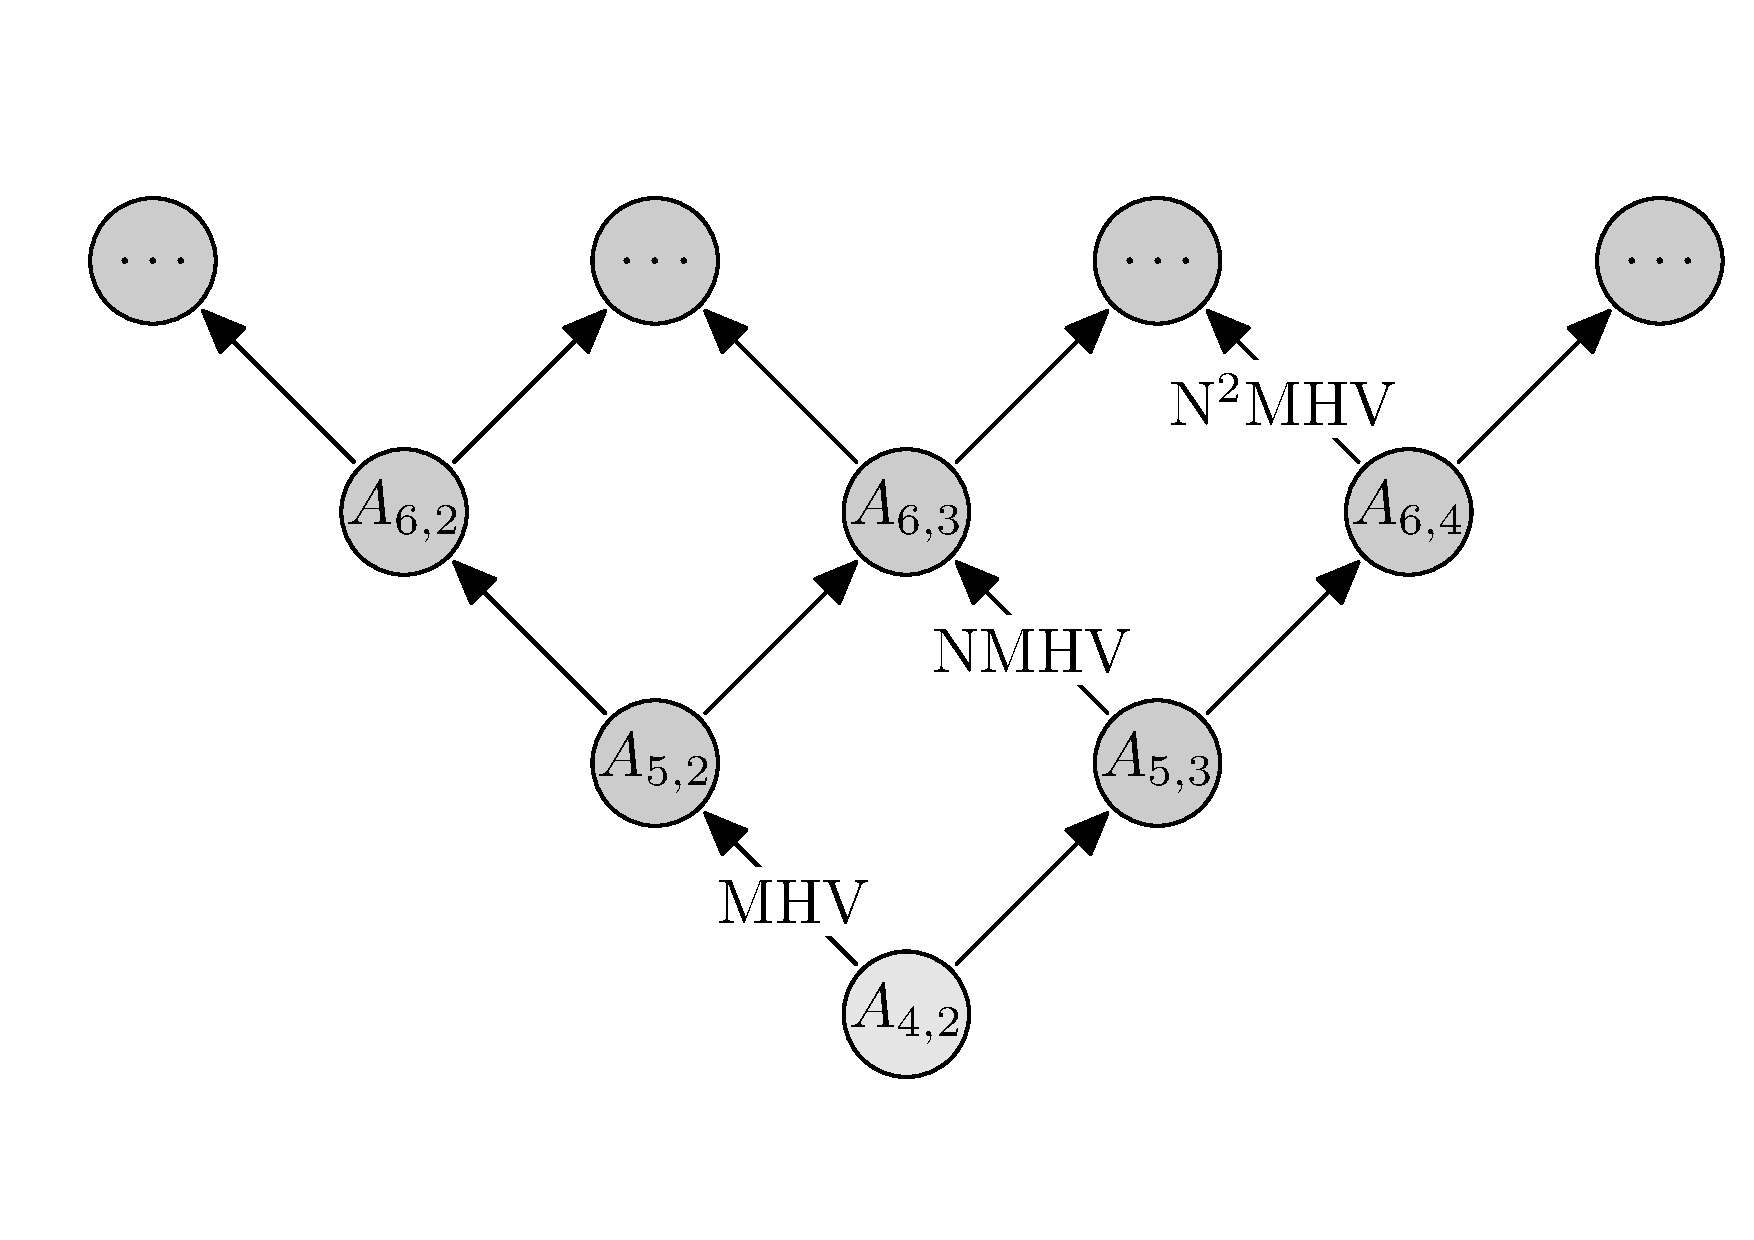
\includegraphics[width=8cm]{ch1_intro/figures/MHV-Pattern.pdf}
\caption{The MHV classification of gluon amplitudes: $A_{n,m}$ denotes an $n$-gluon amplitude
with $m$ positive helicity states. Parity acts as a mirror across the vertical axis as
$A_{n,m} \leftrightarrow A_{n,n-m}$. For example the NMHV $A_{5,3}$ amplitude may be obtained
from the parity mirror of the MHV $A_{5,2}$ one. Hence, the lowest multiplicity non-trivial
NMHV amplitude is the $A_{6,3}$.
 } 
\label{Fig:MHV-Pattern}
\end{figure}

\subsection{The three-gluon tree-amplitudes}

We now want to establish the smallest amplitudes in gluon scattering. As a matter of
fact, three-point amplitudes of massless particles are very special objects. Due to
kinematics all Mandelstam invariants vanish, $p_{i}\cdot p_{j}=0$ for all $i,j$. This follows from 
momentum conservation
\begin{align}
p_{1}^{\mu}+p_{2}^{\mu}+p_{3}^{\mu}=0 \,,
\end{align}
which, with $p_i^2=0$ for all $i$, implies that 
\be
p_{i}\cdot p_{j}=0 \quad \forall \, i,j\in \{1,2,3\} \, .
\ee
%
Hence for real momenta this implies the vanishing of the spinor brackets
$\vev{ij}$ and $\bev{ij}$, which are the building blocks of the amplitudes for massless
particles. There is thus no Lorentz invariant object one could write down, and therefore
the three-particle amplitude must vanish.
The situation is different if one allows for {\it complex momenta} $p_{i} \in {\mathbb{C}^{4}}$.
In this case the helicity spinors
 $\lambda_{i}$ and $\tilde{\lambda}_{i}$ are independent, and the conditions $p_{i} \cdot p_{j} =0 $
can be solved either by $\bev{i j} = 0$
\emph{or} by $\vev{i j} =0$.
Hence either $\tilde\lambda_{1}^{\alpha} \propto \tilde\lambda_{2}^{\alpha} \propto 
\tilde\lambda_{3}^{\alpha}$ (collinear right-handed spinors) or
$\lambda_{1}^{\alpha} \propto \lambda_{2}^{\alpha} \propto 
\lambda_{3}^{\alpha}$ (collinear left-handed spinors) solve the constraints
$p_{i}\cdot p_{j}=0$.
The two choices correspond to the three-gluon MHV${}_{3}$ 
amplitude
\begin{eqnarray}\label{3pointmhv}
A_{3}^{\text{tree}}(1^{-},2^{-},3^{+}) = \i g\frac{ \vev{12}^3 }{\vev{23}\vev{31}}\,,\qquad \lbrack 12\rbrack=\lbrack2 3\rbrack = \lbrack 3 1\rbrack = 0\,, 
\end{eqnarray}
and the dual $\widebar{\text{MHV}}_{3}$ amplitude
\begin{eqnarray} \label{3pointmhvbar}
A_{3}^{\text{tree}}(1^{+},2^{+},3^{-}) = - \i g\frac{ \bev{12}^3 }{\bev{23}\bev{31}}\,,\qquad \vev{1 2}= \vev{2 3} = \vev{3 1} = 0\,, 
\end{eqnarray}
respectively. The two are related by a parity transformation, which flips the helicity weights and exchanges $\spA ij \leftrightarrow [ji]$.

As a useful exercise in spinor gymnastics, we will now 
derive these amplitudes from the colour-ordered Feynman rules.
Using the three-gluon vertex in \eqn{Feynrulveert} we~find  
\begin{align}
   \hspace{-0.2cm} A_{3}^\text{tree}(1^-,2^-,3^+) 
   \!=\!
   \i\frac{g}{\sqrt{2}}\Big[ & (p_1{-}p_2)\!\cdot\!\eps_{+,3} \,  \eps_{-,1}\!\cdot\!\eps_{-,2} 
   \nn\\ & +(p_2{-}p_3)\!\cdot\!\eps_{-,1} \, \eps_{-,2}\!\cdot\!\eps_{+,3} + (p_3{-}p_1)\!\cdot\!
   \eps_{-,2} \,  \eps_{+,3}\!\cdot\!\eps_{-,1}\Big] , 
\end{align}
where the polarisation vector contractions 
are given in \eqn{epscontr}. Choosing the same reference-momentum spinor $\mu_{1}=\mu_{2}=\mu_{3}=\mu$ for the gluons we have $\eps_{-,1} {\cdot} \eps_{-,2} =0$. Then, by using momentum conservation and transversality $p_i\cdot \eps_i=0$, 
we arrive at
\begin{align}
   \hspace{-0.3cm} A_{3}^{\text{tree}}(1^-, 2^-, 3^+) = \i g \sqrt{2} 
   \Big[ p_2\!\cdot\!\eps_{-,1} \, \eps_{-,2}\!\cdot\!\eps_{+,3} -p_1\!\cdot\!\eps_{-,2}\,  \eps_{+,3}\!\cdot\!\eps_{-,1}\Big]\, . 
\end{align}
From \eqn{epscontr} we derive the following expressions,
\begin{align}
\begin{split}
   \eps_{-,2}\!\cdot\!\eps_{+,3}&= -\frac{\lan 2 \mu\ran[3\mu ] }{[ 2 \mu] \lan 3 \mu\ran} \, , \qquad \qquad\, 
   \eps_{-,1}\!\cdot\!\eps_{+,3}= -\frac{\lan 1 \mu\ran[3\mu ] }{[ 1 \mu] \lan 3 \mu\ran} \, , 
   \\
     p_2\cdot \eps_{-,1}&= \frac{1}{\sqrt{2}}\frac{\lan 12 \ran[2 \mu]}{[1 \mu]}\, , \qquad \quad\ \ \,
     p_1\cdot \eps_{-,2}= -\frac{1}{\sqrt{2}}\frac{\lan 12 \ran[1 \mu]}{[2 \mu]}\, ,
     \end{split}
\end{align}
and therefore
\begin{align}
\begin{split}
    A_{3}^{\text{tree}}(1^-, 2^-, 3^+) &= -\i g \lan 12\ran \frac{[3\mu]}{\lan 3\mu\ran}
   \left(  \frac{\lan 2\mu\ran}{[1\mu]} +\frac{\lan 1\mu\ran}{[2\mu]}  \right) \\ & = 
    \i g \lan 12\ran \frac{[3\mu]}{\lan 3\mu\ran}
   \frac{\lan \mu | \slashed{p}_1 + \slashed{p}_2 |\mu] 
  % \lan 1\mu\ran [1\mu]+ \lan 2\mu\ran [2\mu]  
  }{[1\mu][2\mu]}
  %\\&
  =
  \i g \frac{\lan 12\ran [3\mu]^2 }{[1\mu][2\mu]}
   \, . 
   \end{split}
\end{align}
Finally, we use three-point momentum conservation to simplify
\begin{align}
\frac{[3\mu] }{[1\mu]}=\frac{\lan 23\ran [3\mu] }{\lan 23\ran[1\mu]}=\frac{\lan12\ran}{\lan23\ran}\, , \qquad \quad 
\frac{[3\mu] }{[2\mu]}=\frac{\lan 13\ran [3\mu] }{\lan 13\ran[2\mu]}=\frac{\lan12\ran}{\lan31\ran}\, ,
    \end{align}
    thus arriving at the result in \eqn{3pointmhv}. One could repeat this calculation for the scattering of three gravitons, this time using the three-graviton vertex of \eqn{3gravitonvertex}, arriving at a result proportional to  $\big[ A_{3}^{\text{tree}}(1^{-}, 2^{-}, 3^{+})\big]^2$. The involved expression for the vertex \eqn{3gravitonvertex} 
    gives no hints of such a remarkable squaring relation! 
    We shall take up this discussion in chapter~\ref{ch:trees} again.
    
\subsection{Helicity weight}
\label{sec:helscale}

There is an important consistency requirement for scattering amplitudes based on
checking their correct helicity weights.
This  is encoded in the following relation~\cite{ch1_Witten:2003nn}:
\begin{align}
\label{lg}
   \hat h_{i}\, A=  -\frac{1}{2} \left( \lambda_i^\alpha \ \frac{\partial}{\partial \lambda_i^\alpha} - \tilde{\lambda}_i^{\dot{\alpha}}\frac{\partial}{\partial \tilde{\lambda}_i^{\dot{\alpha}}}\right) \, A \, = \, h_i \, A\, , 
\end{align}
where $h_i$ is the helicity of particle $i$. 
When combined with Lorentz invariance, this relation can be used to determine the functional form of the three-point amplitudes of particles of any spin. As we argued, above a massless
three-particle amplitude in complexified momentum space can either only depend on $\langle i\, j\rangle$ with $[ i\, j] {=}0$ for all particles or vice versa.
If we choose the MHV situation $[ i\, j] {=}0$ for the helicity assignment $1^{-s}, 2^{-s}, 3^{+s}$, one can immediately see, using \eqref{lg}, that the answer must have the form  
\begin{align}
\label{generalsMHV}
        A(1^{-s}, 2^{-s}, 3^{+s}) \sim  \big[ A(1^{-}, 2^{-}, 3^{+})\big]^s\, .
\end{align}
In fact, for the gluon-amplitude with $s{=}1$, the conditions
\be
\hat h_{1} A_{3}^{\text{MHV}}= - A_{3}^{\text{MHV}}\, , \quad
\hat h_{2} A_{3}^{\text{MHV}}= - A_{3}^{\text{MHV}}\, , \quad
\hat h_{3} A_{3}^{\text{MHV}}= + A_{3}^{\text{MHV}}\,  \quad
\ee
uniquely fix the amplitude to take the form
 $A(1^-, 2^-, 3^+) \!\sim\!{\langle 1\, 2\rangle^3}/ ({\langle 2\, 3\rangle\langle 3\, 1\rangle})$.
This may be seen as an independent derivation of both the 3-point gluon and graviton
amplitudes---without referring to any Lagrangian!


\begin{exer}{The $\widebar{\text{MHV}}_{3}$ amplitude}
\label{Ex:MHV3}
Derive the anti-MHV three-gluon amplitude~\eqref{3pointmhvbar} using the colour-ordered Feynman rules.
For the solution see \hyperref[Sol:MHV3]{chapter~5}.
\end{exer}


\begin{example}{Example: A four-gluon tree-amplitude}
%\label{sec:four-gluon-example}

We shall now compute the simplest non-trivial tree-level colour-ordered gluon amplitude, namely the 
four-gluon MHV-amplitude with a split helicity distribution $A_{4}^{\text{tree}}(1^{-},2^{-},3^{+},4^{+})$.
Employing the colour-ordered Feynman rules of \eqn{Feynrulveert} we see
that the three diagrams of figure~\ref{fig:4gluon} contribute to the amplitude.
%
\begin{figure}[t]
   \centering
    \begin{equation*}
    A_{4}^{\text{tree}}(1^-,2^-,3^+,4^+)=
 \begin{tikzpicture}[baseline={(current bounding box.center)}]
  \begin{feynman}
    \coordinate (t) at (-0.8,0.8);
    \coordinate (d) at (-0.8,-0.8);
        \coordinate (a) at (-0.4,0);
                \coordinate (b) at (0.4,0);
           \coordinate (ot) at (0.8,0.8);
                      \coordinate (od) at (0.8,-0.8);
                       \coordinate (T) at (0,-1); \draw (T) node [below] {(I)};
         \draw [gluon] (t) -- (a);
          \draw [gluon] (a) -- (d);
         \draw [gluon] (ot) -- (b);
          \draw [gluon] (a) -- (b);
          \draw [gluon] (b) -- (od);          
               \draw [fill] (a) circle (.08); \draw [fill] (b) circle (.08);
    \draw (ot) node [right] {$3^{+}$};
          \draw (t) node [left] {$2^{-}$};
               \draw (d) node [left] {$1^{-}$};
                      \draw (od) node [right] {$4^{+}$};
                      \end{feynman}
      \end{tikzpicture}
 +    
  \begin{tikzpicture}[baseline={(current bounding box.center)}]
  \begin{feynman}
    \coordinate (t) at (-0.8,0.8);
    \coordinate (d) at (-0.8,-0.8);
        \coordinate (a) at (0,0.4);
                \coordinate (b) at (0,-0.4);
           \coordinate (ot) at (0.8,0.8);
                      \coordinate (od) at (0.8,-0.8);
                       \coordinate (T) at (0,-1); \draw (T) node [below] {(II)};
         \draw [gluon] (t) -- (a);
          \draw [gluon] (b) -- (d);
         \draw [gluon] (ot) -- (a);
          \draw [gluon] (a) -- (b);
          \draw [gluon] (b) -- (od);          
               \draw [fill] (a) circle (.08); \draw [fill] (b) circle (.08);
    \draw (ot) node [right] {$3^{+}$};
          \draw (t) node [left] {$2^{-}$};
               \draw (d) node [left] {$1^{-}$};
                      \draw (od) node [right] {$4^{+}$};
                      \end{feynman}
      \end{tikzpicture}
+
  \begin{tikzpicture}[baseline={(current bounding box.center)}]
  \begin{feynman}
    \coordinate (t) at (-0.8,0.8);
    \coordinate (d) at (-0.8,-0.8);
        \coordinate (a) at (0,0);
           \coordinate (ot) at (0.8,0.8);
                      \coordinate (od) at (0.8,-0.8);
                       \coordinate (T) at (0,-1); \draw (T) node [below] {(III)};
         \draw [gluon] (t) -- (a);
          \draw [gluon] (a) -- (d);
         \draw [gluon] (ot) -- (a);
          \draw [gluon] (a) -- (od);          
               \draw [fill] (a) circle (.08);
     \draw (ot) node [right] {$3^{+}$};
          \draw (t) node [left] {$2^{-}$};
               \draw (d) node [left] {$1^{-}$};
                      \draw (od) node [right] {$4^{+}$};
                      \end{feynman}
      \end{tikzpicture}
   \end{equation*}
   \caption{The three colour-ordered graphs contributing to the four-gluon split helicity
    MHV amplitude.}
   \label{fig:4gluon}
\end{figure}
%
Its computation is again considerably simplified by a clever choice of the reference momenta $r_i=\mu_{i}\,
\tilde\mu_{i}$ of the gluon polarisations,
\be
r_{1}=r_{2}=p_{4}\, , \qquad r_{3}=r_{4}=p_{1} \, ,
\label{polchoice}
\ee
where $p_{i}$ denote the physical external momenta. Then one sees, using~\eqn{epscontr}, that the polarisation-vector products
\be
\epsilon_{-, 1}\cdot\epsilon_{-, 2}   = \epsilon_{+, 3}\cdot\epsilon_{+, 4} =
\epsilon_{-, 1}\cdot\epsilon_{+, 4}  =  \epsilon_{-, 2}\cdot\epsilon_{+, 4} =
\epsilon_{-, 1}\cdot\epsilon_{+, 3}  = 0 
\label{eezero}
\ee
all vanish, and that the \emph{only} non-vanishing contraction is 
\be
\label{e2e3}
\epsilon_{-, 2}\cdot\epsilon_{+, 3}   =  - \frac{\vev{\mu_{3}\,\lambda_{2}} \, \bev{\mu_{2}\, \lambda_{3}}}
{\vev{\la_{3}\, \mu_{3}}\, \bev{\la_{2}\, \mu_{2}}} = - \frac{\vev{12}\, \bev{34}}{\vev{13}\,\bev{24}}\, .
\ee
Of course it is mandatory to use the same choice of reference momenta for all~graphs. 

\newpage

\begin{trailer}{Diagram I:}
%
\begin{align}
\begin{aligned}
(\text{I}) = \left(\frac{\i g}{\sqrt{2}}\right )^{2}\, \frac{-\i\,\eta_{\mu\nu}}{s_{12}}\, & \Bigl [
\epsilon_{-,2}^{\mu} \, (p_{2q}\cdot \epsilon_{-,1}) + \epsilon_{-,1}^{\mu} \, (p_{q1}\cdot \epsilon_{-,2})\, 
\Bigr ] \\
\times \Bigl [
\epsilon_{+,4}^{\nu} \, & (p_{4(-q)}\cdot \epsilon_{+,3}) + \epsilon_{+,3}^{\nu} \, (p_{(-q)3}\cdot \epsilon_{+,4})\, 
\Bigr ] \, ,
\end{aligned}
\end{align}
with $q=-p_{1}-p_{2}=p_{3}+p_{4}$, $s_{12}=(p_{1}+p_{2})^{2}=\vev{12}\bev{21}$ and $p_{ij}=p_{i}-p_{j}$. 
Due to only $\epsilon_{-,2}\cdot\epsilon_{+,3}$ surviving in the contraction, we have
\begin{align} \begin{aligned}
(\text{I}) & = \frac{\i g^{2}}{2s_{12}}\, (\epsilon_{-,2}\cdot\epsilon_{+,3})\, (p_{2}+p_{1}+p_{2})\cdot\epsilon_{-,1}\,
(-p_{3}-p_{4}-p_{3})\cdot\epsilon_{+,4} \\ 
 & = -\frac{2\i g^{2}}{s_{12}}\,(\epsilon_{-, 2}\cdot\epsilon_{+, 3})\,(p_{2}\cdot\epsilon_{-, 1})\, 
 (p_{3}\cdot\epsilon_{+, 4}) \\ 
 & = - \frac{2\i g^{2}}{s_{12}}\, \left ( - \frac{\vev{12}\, \bev{34}}{\vev{13}\, \bev{24}}\, \right )\,
  \left ( \frac{1}{\sqrt{2}}\, \frac{\vev{12}\, \bev{24}}{\bev{14}}\, \right )\,
   \left ( \frac{1}{\sqrt{2}}\, \frac{\vev{13}\, \bev{34}}{\vev{14}}\, \right ) \\
& = \i g^{2}\, \frac{\vev{12}\, \bev{34}^{2}}{\bev{12}\, \vev{14}\, \bev{41}}\, ,
\end{aligned} \end{align} 
where in the second line we used  $\displaystyle p_{2}\cdot \epsilon_{-,1}= \ft{1}{\sqrt{2}}\, \ft{\vev{12}\, 
\bev{2\,\mu_{1}}}{\bev{1\mu_{1}}} \stackrel{\mu_{1}=4}{=} \ft{1}{\sqrt{2}}\, \ft{\vev{12}\, 
\bev{24}}{\bev{14}}$, and similarly for $p_{3}\cdot \epsilon_{+,4}$. The last expression can be rewritten
exclusively in terms of $\lambda_{i}$ spinors~as
\begin{align} \begin{aligned}
-\ft{\i}{g^{2}}\, (\text{I})&=
\frac{\vev{12}\, \bev{34}^{2}}{\bev{12}\, \vev{14}\, \bev{41}} \frac{\vev{43}}{\vev{43}} =
\frac{\vev{12}\, \bev{34}}{\bev{12}\, \vev{14}}\,  \frac{ \overbrace{ \bev{34}\, \vev{43}}^{\vev{12}\,\bev{21}}}
{ \underbrace{\vev{43}\, \bev{41}}_{\hspace{-0.5cm} -\vev{34}\,\bev{41}=\vev{32}\,\bev{21} \hspace{-0.5cm}}} =
\frac{-\vev{12}^{2}}{\vev{23}\, \vev{41}}\, \underbrace{\frac{\bev{34}}{\bev{21}}}_{\frac{\vev{12}}{\vev{43}}} \\ 
& = \frac{\vev{12}^{3}}{\vev{23}\, \vev{34}\, \vev{41}} \, .
\end{aligned} \end{align}
%
Here in the first step the four-point kinematical relation $s_{12}=\vev{12}\,\bev{21}=s_{34}=\vev{34}\,\bev{43}$
was used.
\end{trailer}

\newpage 

\begin{trailer}{Diagram II:}
Using again the fact that the only non-vanishing contraction is that of \eqn{e2e3} we
find a vanishing result:
\begin{align}
(\text{II})  & \propto \frac{-\i}{2s_{14}}\, 
(\epsilon_{2}\cdot\epsilon_{3})\, \Bigl [\, (p_{23}\cdot\epsilon_{1})\, (p_{1(-q)}\cdot\epsilon_{4})
+ (p_{23}\cdot\epsilon_{4})\, (p_{(-q)4}\cdot\epsilon_{1}) \, \Bigr ] =0\, .
\end{align}
Here with $q=p_{1}+p_{4}$ we have $p_{1(-q)}\cdot\epsilon_{4}=2\, p_{1}\cdot\epsilon_{4}=0$, which vanishes
by virtue of our choice $q_{4}=p_{1}$ of \eqn{polchoice}. Similarly, 
$p_{(-q)4}\cdot\epsilon=-2\, p_{4}\cdot\epsilon_1 =0$ as $q_{1}=p_{4}$. 
Hence diagram II gives no contribution. 
\end{trailer}

\begin{trailer}{Diagram III:}
The same holds true for the third graph as
\begin{align}
(\text{III})\propto 2\, (\epsilon_{2}\cdot\epsilon_{4})\, (\epsilon_{1}\cdot\epsilon_{3})
- (\epsilon_{2}\cdot\epsilon_{3})\, (\epsilon_{1}\cdot\epsilon_{4})-
 (\epsilon_{2}\cdot\epsilon_{1})\, (\epsilon_{3}\cdot\epsilon_{4}) = 0 \, ,
\end{align}
where at least one of the vanishing contractions in~\eqn{eezero} appears in each term.
\end{trailer}

In summary, we have established the following compact result for the split-helicity MHV four-point amplitude:
\be
A_{4}^{\text{tree}}(1^{-},2^{-},3^{+},4^{+}) = \i g^{2}\frac{\vev{12}^{4}}{\vev{12}\,\vev{23}\, \vev{34}\, \vev{41}} \, .
\label{MHV4g1}
\ee
At this point it is also instructive to check the helicity weights of our final result 
for every leg using the helicity generator of \eqn{lg}. To wit,
$$
\hat{h}_{1}\,A_{4}=\ft 1 2\,(-4+2)\, A_{4}= -A_{4}\, , \quad \ \hat{h}_{2}\, A_{4}=-A_{4} \, ,\quad \ h_{3}\, A_{4}=+A_{4}\, ,\quad
\ \hat{h}_{4}\, A_{4}=+A_{4}\, ,
\label{helicitycheck}
$$
so everything is in order.

\smallskip

By cyclicity there is only one more independent four-gluon amplitude left to compute: the 
case $A_{4}^{\text{tree}}(1^{-},2^{+},3^{-},4^{+})$ with an alternating
helicity distribution. All other possible helicity distributions can be
related to this or  $A_{4}^{\text{tree}}(1^{-},2^{-},3^{+},4^{+})$ of \eqn{MHV4g1} by cyclicity. 
It turns out that we do not need to do another Feynman diagrammatic
computation, as the missing amplitude follows from the $\text{U}(1)$ decoupling theorem of 
\eqn{U1decoupling}:
\begin{align}
\begin{aligned}
A_{4}^{\text{tree}}(1^{-},2^{+},3^{-},4^{+}) & = - A_{4}^{\text{tree}}(1^{-},2^{+},4^{+},3^{-}) - A_{4}^{\text{tree}}(1^{-},4^{+},2^{+},3^{-})  \\
& = -\i g^{2}\left ( \frac{\vev{31}^{4}}{\vev{12}\,\vev{24}\,\vev{43}\, \vev{31}} + 
 \frac{\vev{31}^{4}}{\vev{14}\,\vev{42}\,\vev{23}\, \vev{31}} \right ) \\
 & = \i g^{2} \frac{\vev{31}^{4}}{\vev{12}\,\vev{23}\,\vev{34}\, \vev{41}} \, .
\end{aligned} \end{align}
Comparing this result to \eqn{MHV4g1} we may express all four-gluon MHV amplitudes in a single
and crafty formula,
\be
A^{\text{tree}}_{4}(\ldots i^{-}\ldots j^{-}\ldots) = \i g^{2} 
\, \frac{\vev{ij}^{4}}{\vev{12}\,\vev{23}\,\vev{34}\, \vev{41}}
\, ,
\label{I.35}
\ee
where the dots stand for positive-helicity gluon states. 



In fact we shall show in chapter~\ref{ch:trees} that this formula has a straightforward generalisation to the $n$-gluon MHV case, in which only the denominator is modified~to
\be
A^{\text{tree}}_{n}(\ldots i^{-}\ldots j^{-}\ldots) =  \i g^{n-2} 
\, \frac{\vev{ij}^{4}}{\vev{12}\,\vev{23}\ldots\,\vev{(n-1)n}\, \vev{n1}}
\, ,
\label{ParkeTaylor1}
\ee
known as the Parke-Taylor amplitude~\cite{ch1_Parke:1986gb}. It is a remarkably simple and closed
expression for a tree-level amplitude with an arbitrary number $n$ of gluons.
We shall derive it in the next chapter.

By parity this results implies the $n$-gluon $\widebar{\text{MHV}}$ amplitudes 
\be
A^{\text{tree}}_{n}(\ldots i^{+}\ldots j^{+}\ldots) = (-1)^{n} \i g^{n-2} 
\, \frac{\bev{ij}^{4}}{\bev{12}\,\bev{23}\ldots\,\bev{(n-1)n}\, \bev{n1}}
\, ,
\label{ParkeTaylor1MHVbar}
\ee
in agreement with the result of exercise~\ref{Ex:MHV3} for the $n=3$ case.

\end{example}

 

\begin{exer}{Four-point quark-gluon scattering}
\label{Ex:1.11}
Show, by using the colour-ordered Feynman rules and a suitable choice for the gluon-polarisation 
reference vector
$r_{3}^{\a\da}=\mu_{3}^{\a}\, \tilde\mu_{3}^{\da}$,
that the first non-trivial $\bar q q g g$ scattering amplitude is given by
\be
\label{qqgg-amp}
A_{\bar q q  gg}^{\text{tree}}(1^{-}_{\bar q}, 2^{+}_{q}, 3^{-},4^{+}) = -\i g^{2}
\frac{\vev{13}^{3}\, \vev{23}}
{\vev{12}\,\vev{23}\,\vev{34}\, \vev{41}}\, .
\ee
Also convince yourself that the result for this amplitude has the correct helicity assignments, as we did in
\eqn{helicitycheck} for the pure-gluon case.
For the solution see \hyperref[Sol:1.11]{chapter~5}.
\end{exer}

\subsection{Vanishing graviton tree-amplitudes}

The observation of section~\ref{sec:mostlyplus} that the mostly-plus gluon amplitudes
vanish, $A_{n}(1^{+},\ldots, n^{+})=0=A_{n}(1^{-},2^{+},\ldots, n^{+})$, carries over
to the graviton case as well:
\be
\label{Mmostlyplus}
M_{n}(1^{++},\ldots, n^{++})=0=M_{n}(1^{--},2^{++},\ldots, n^{++}) \,.
\ee
The proof is completely analogous. Recall the representation of the graviton
polarisation tensor
as a product of two spin-1 polarisations in \eqn{gravitonpolarize}:
%
\be
\epsilon_{\mu\nu, \, i}^{\pm\pm}=\epsilon_{\mu, \, i}^{\pm}\, \epsilon_{\nu, \, i}^{\pm}
\qquad i=1,\ldots , n \, .
\ee
%
Again suitable choices for the reference momenta $r_{i}$ allow us to set to zero all possible $\epsilon^{\mu\nu}_{i} \epsilon_{j, \, \mu\nu}$
contractions 
for the two mostly-plus helicity configurations of \eqn{Mmostlyplus}.
%
\smallskip
\begin{enumerate}[i)]
\item $M_{n}(1^{++},\ldots, n^{++})$: 
Here we choose all reference momenta uniformly $r_{i}=r$ $\forall i$ with $r\neq p_{i}$
$\forall i\in \{1,\ldots, n\}$. This implies that all contractions
\be
\epsilon^{\mu\nu\, ++}_{i} \epsilon_{j, \, \mu\nu}^{++}=(\epsilon^{+}_{i}\cdot 
\epsilon^{+}_{j})^{2}=0
\ee
vanish by virtue of \eqref{s1polarrel}.

\smallskip
\item $M_{n}(1^{--},2^{++},\ldots, n^{++})$: 
Here we choose $r_{1}\neq p_{1}$ arbitrarily, and the remaining $r_{i}=p_{1}$ uniformly $\forall 
i\in \{2,\ldots, n\}$. This entails $\epsilon^{-}_{1}\cdot \epsilon^{+}_{i}=0$ as well as
$\epsilon^{+}_{i}\cdot \epsilon^{+}_{j}=0$, and the analogue for the graviton polarisation
contractions,
\be
\epsilon^{--}_{1}\cdot \epsilon^{++}_{i}=0=\epsilon^{++}_{i}\cdot \epsilon^{++}_{j}=0\, ,
\qquad \forall 
i,j\in \{2,\ldots, n\}\,.
\ee 
\end{enumerate}
%
In order to show the vanishing of these amplitudes we need to ensure that in every term comprising a
mostly-plus graviton tree-level amplitude there is at least one polarisation-tensor contraction
$\epsilon^{\mu\nu}_{i} \epsilon_{j, \, \mu\nu}$. This is easy to show: as we saw in the discussion
of section~\ref{sec:1.6}, \emph{all} multi-graviton vertices scale homogeneously quadratically in the momenta
due to $\sqrt{g} \, R \sim \sum_{n} \partial^{2} h^{n}$. Therefore, the maximum number of momenta in the numerator
of an $n$-graviton tree-level scattering amplitude arises from pure three-graviton vertex graphs.
These graphs contain $n-2$ three-vertices, hence the counting for these yields a total of $2(n-1)$ momenta
and $n$ graviton polarisation tensors, each one splitting up into a product
of two polarisation vectors.
Looking at the possible contractions of this set of $2(n-1)$ momentum vectors and
$2n$ polarisation vectors we see that at least one contraction of the type
$\epsilon_{i}\cdot\epsilon_{j}$ must happen. As these may be set to zero through
 a suitable choice of
 reference momenta, this proves the vanishing graviton trees of
 \eqn{Mmostlyplus}.


\begin{thebibliography}{99.}%
%\cite{Ramond:1981pw}
\bibitem{ch1_Ramond:1981pw}
P.~Ramond,
``Field theory. A modern primer,''
Front. Phys. \textbf{51} (1981), 1--397.

%\cite{Weinberg:1995mt}
\bibitem{ch1_Weinberg:1995mt}
S.~Weinberg,
``The Quantum theory of fields. Vol. 1: Foundations,''
Cambridge University Press, 2005,
ISBN 978-0-521-67053-1, 978-0-511-25204-4
doi:10.1017/CBO9781139644167.

%\cite{Schwartz:2014sze}
\bibitem{ch1_Schwartz:2014sze}
M.~D.~Schwartz,
``Quantum Field Theory and the Standard Model,''
Cambridge University Press, 2014,
ISBN 978-1-107-03473-0, 978-1-107-03473-0.

%\cite{Yang:1954ek}
\bibitem{ch1_Yang:1954ek}
C.~N.~Yang and R.~L.~Mills,
``Conservation of Isotopic Spin and Isotopic Gauge Invariance,''
Phys. Rev. \textbf{96} (1954), 191-195
doi:10.1103/PhysRev.96.191.

%\cite{Cvitanovic:1976am}
\bibitem{ch1_Cvitanovic:1976am}
P.~Cvitanovic,
``Group theory for Feynman diagrams in non-Abelian gauge theories,''
Phys. Rev. D \textbf{14} (1976), 1536-1553
doi:10.1103/PhysRevD.14.1536.

%\cite{Donoghue:1994dn}
\bibitem{ch1_Donoghue:1994dn}
J.~F.~Donoghue,
``General relativity as an effective field theory: The leading quantum corrections,''
Phys. Rev. D \textbf{50} (1994), 3874-3888
doi:10.1103/PhysRevD.50.3874
[arXiv:gr-qc/9405057 [gr-qc]].

%\cite{Goldberger:2004jt}
\bibitem{ch1_Goldberger:2004jt}
W.~D.~Goldberger and I.~Z.~Rothstein,
``An Effective field theory of gravity for extended objects,''
Phys. Rev. D \textbf{73} (2006), 104029
doi:10.1103/PhysRevD.73.104029
[arXiv:hep-th/0409156 [hep-th]].

%\cite{Bern:2019crd}
\bibitem{ch1_Bern:2019crd}
Z.~Bern, C.~Cheung, R.~Roiban, C.~H.~Shen, M.~P.~Solon and M.~Zeng,
``Black Hole Binary Dynamics from the Double Copy and Effective Theory,''
JHEP \textbf{10} (2019), 206
doi:10.1007/JHEP10(2019)206
[arXiv:1908.01493 [hep-th]].

%\cite{Mogull:2020sak}
\bibitem{ch1_Mogull:2020sak}
G.~Mogull, J.~Plefka and J.~Steinhoff,
``Classical black hole scattering from a worldline quantum field theory,''
JHEP \textbf{02} (2021), 048
doi:10.1007/JHEP02(2021)048
[arXiv:2010.02865 [hep-th]].

%\cite{Sannan:1986tz}
\bibitem{ch1_Sannan:1986tz}
S.~Sannan,
``Gravity as the Limit of the Type {II} Superstring Theory,''
Phys. Rev. D \textbf{34} (1986), 1749
doi:10.1103/PhysRevD.34.1749.

%\cite{Mangano:1990by}
\bibitem{ch1_Mangano:1990by}
M.~L.~Mangano and S.~J.~Parke,
``Multiparton amplitudes in gauge theories,''
Phys. Rept. \textbf{200} (1991), 301-367
doi:10.1016/0370-1573(91)90091-Y
[arXiv:hep-th/0509223 [hep-th]].

%\cite{Ita:2011ar}
\bibitem{ch1_Ita:2011ar}
H.~Ita and K.~Ozeren,
``Colour Decompositions of Multi-quark One-loop QCD Amplitudes,''
JHEP \textbf{02} (2012), 118
doi:10.1007/JHEP02(2012)118
[arXiv:1111.4193 [hep-ph]].

%\cite{Badger:2012pg}
\bibitem{ch1_Badger:2012pg}
S.~Badger, B.~Biedermann, P.~Uwer and V.~Yundin,
``Numerical evaluation of virtual corrections to multi-jet production in massless QCD,''
Comput. Phys. Commun. \textbf{184} (2013), 1981-1998
doi:10.1016/j.cpc.2013.03.018
[arXiv:1209.0100 [hep-ph]].

%\cite{Reuschle:2013qna}
\bibitem{ch1_Reuschle:2013qna}
C.~Reuschle and S.~Weinzierl,
``Decomposition of one-loop QCD amplitudes into primitive amplitudes based on shuffle relations,''
Phys. Rev. D \textbf{88} (2013) no.10, 105020
doi:10.1103/PhysRevD.88.105020
[arXiv:1310.0413 [hep-ph]].

%\cite{Bern:1990ux}
\bibitem{ch1_Bern:1990ux}
Z.~Bern and D.~A.~Kosower,
``Color decomposition of one loop amplitudes in gauge theories,''
Nucl. Phys. B \textbf{362} (1991), 389-448
doi:10.1016/0550-3213(91)90567-H.

%\cite{DelDuca:1999rs}
\bibitem{ch1_DelDuca:1999rs}
V.~Del Duca, L.~J.~Dixon and F.~Maltoni,
``New color decompositions for gauge amplitudes at tree and loop level,''
Nucl. Phys. B \textbf{571} (2000), 51-70
doi:10.1016/S0550-3213(99)00809-3
[arXiv:hep-ph/9910563 [hep-ph]].

%\cite{Kleiss:1988ne}
\bibitem{ch1_Kleiss:1988ne}
R.~Kleiss and H.~Kuijf,
``Multi - Gluon Cross-sections and Five Jet Production at Hadron Colliders,''
Nucl. Phys. B \textbf{312} (1989), 616-644
doi:10.1016/0550-3213(89)90574-9.

%\cite{Bern:2008qj}
\bibitem{ch1_Bern:2008qj}
Z.~Bern, J.~J.~M.~Carrasco and H.~Johansson,
``New Relations for Gauge-Theory Amplitudes,''
Phys. Rev. D \textbf{78} (2008), 085011
doi:10.1103/PhysRevD.78.085011
[arXiv:0805.3993 [hep-ph]].

%\cite{Bern:2010ue}
\bibitem{ch1_Bern:2010ue}
Z.~Bern, J.~J.~M.~Carrasco and H.~Johansson,
``Perturbative Quantum Gravity as a Double Copy of Gauge Theory,''
Phys. Rev. Lett. \textbf{105} (2010), 061602
doi:10.1103/PhysRevLett.105.061602
[arXiv:1004.0476 [hep-th]].

%\cite{Johansson:2015oia}
\bibitem{ch1_Johansson:2015oia}
H.~Johansson and A.~Ochirov,
``Color-Kinematics Duality for QCD Amplitudes,''
JHEP \textbf{01} (2016), 170
doi:10.1007/JHEP01(2016)170
[arXiv:1507.00332 [hep-ph]].

%\cite{Melia:2015ika}
\bibitem{ch1_Melia:2015ika}
T.~Melia,
``Proof of a new colour decomposition for QCD amplitudes,''
JHEP \textbf{12} (2015), 107
doi:10.1007/JHEP12(2015)107
[arXiv:1509.03297 [hep-ph]].

%\cite{Dixon:1996wi}
\bibitem{ch1_Dixon:1996wi}
L.~J.~Dixon,
``Calculating scattering amplitudes efficiently,''
[arXiv:hep-ph/9601359 [hep-ph]].

%\cite{Henn:2014yza}
\bibitem{ch1_Henn:2014yza}
J.~M.~Henn and J.~C.~Plefka,
``Scattering Amplitudes in Gauge Theories,''
Lect. Notes Phys. \textbf{883} (2014), pp.1-195
Springer, 2014,
ISBN 978-3-642-54021-9
doi:10.1007/978-3-642-54022-6.

%\cite{Witten:2003nn}
\bibitem{ch1_Witten:2003nn}
E.~Witten,
``Perturbative gauge theory as a string theory in twistor space,''
Commun. Math. Phys. \textbf{252} (2004), 189-258
doi:10.1007/s00220-004-1187-3
[arXiv:hep-th/0312171 [hep-th]].

%\cite{Parke:1986gb}
\bibitem{ch1_Parke:1986gb}
S.~J.~Parke and T.~R.~Taylor,
``An Amplitude for $n$ Gluon Scattering,''
Phys. Rev. Lett. \textbf{56} (1986), 2459
doi:10.1103/PhysRevLett.56.2459.
\end{thebibliography}